% Options for packages loaded elsewhere
\PassOptionsToPackage{unicode}{hyperref}
\PassOptionsToPackage{hyphens}{url}
\PassOptionsToPackage{dvipsnames,svgnames,x11names}{xcolor}
%
\documentclass[
  letterpaper,
  11pt,
  english,
  onehalfspacing,
  headsepline]{MastersDoctoralThesis}

\usepackage{amsmath,amssymb}
\usepackage{iftex}
\ifPDFTeX
  \usepackage[T1]{fontenc}
  \usepackage[utf8]{inputenc}
  \usepackage{textcomp} % provide euro and other symbols
\else % if luatex or xetex
  \usepackage{unicode-math}
  \defaultfontfeatures{Scale=MatchLowercase}
  \defaultfontfeatures[\rmfamily]{Ligatures=TeX,Scale=1}
\fi
\usepackage{lmodern}
\ifPDFTeX\else  
    % xetex/luatex font selection
\fi
% Use upquote if available, for straight quotes in verbatim environments
\IfFileExists{upquote.sty}{\usepackage{upquote}}{}
\IfFileExists{microtype.sty}{% use microtype if available
  \usepackage[]{microtype}
  \UseMicrotypeSet[protrusion]{basicmath} % disable protrusion for tt fonts
}{}
\makeatletter
\@ifundefined{KOMAClassName}{% if non-KOMA class
  \IfFileExists{parskip.sty}{%
    \usepackage{parskip}
  }{% else
    \setlength{\parindent}{0pt}
    \setlength{\parskip}{6pt plus 2pt minus 1pt}}
}{% if KOMA class
  \KOMAoptions{parskip=half}}
\makeatother
\usepackage{xcolor}
\usepackage[paper=a4paper,inner=2.5cm,outer=3.8cm,bindingoffset=.5cm,top=1.5cm,bottom=1.5cm]{geometry}
\setlength{\emergencystretch}{3em} % prevent overfull lines
\setcounter{secnumdepth}{5}
% Make \paragraph and \subparagraph free-standing
\ifx\paragraph\undefined\else
  \let\oldparagraph\paragraph
  \renewcommand{\paragraph}[1]{\oldparagraph{#1}\mbox{}}
\fi
\ifx\subparagraph\undefined\else
  \let\oldsubparagraph\subparagraph
  \renewcommand{\subparagraph}[1]{\oldsubparagraph{#1}\mbox{}}
\fi


\providecommand{\tightlist}{%
  \setlength{\itemsep}{0pt}\setlength{\parskip}{0pt}}\usepackage{longtable,booktabs,array}
\usepackage{calc} % for calculating minipage widths
% Correct order of tables after \paragraph or \subparagraph
\usepackage{etoolbox}
\makeatletter
\patchcmd\longtable{\par}{\if@noskipsec\mbox{}\fi\par}{}{}
\makeatother
% Allow footnotes in longtable head/foot
\IfFileExists{footnotehyper.sty}{\usepackage{footnotehyper}}{\usepackage{footnote}}
\makesavenoteenv{longtable}
\usepackage{graphicx}
\makeatletter
\def\maxwidth{\ifdim\Gin@nat@width>\linewidth\linewidth\else\Gin@nat@width\fi}
\def\maxheight{\ifdim\Gin@nat@height>\textheight\textheight\else\Gin@nat@height\fi}
\makeatother
% Scale images if necessary, so that they will not overflow the page
% margins by default, and it is still possible to overwrite the defaults
% using explicit options in \includegraphics[width, height, ...]{}
\setkeys{Gin}{width=\maxwidth,height=\maxheight,keepaspectratio}
% Set default figure placement to htbp
\makeatletter
\def\fps@figure{htbp}
\makeatother
\newlength{\cslhangindent}
\setlength{\cslhangindent}{1.5em}
\newlength{\csllabelwidth}
\setlength{\csllabelwidth}{3em}
\newlength{\cslentryspacingunit} % times entry-spacing
\setlength{\cslentryspacingunit}{\parskip}
\newenvironment{CSLReferences}[2] % #1 hanging-ident, #2 entry spacing
 {% don't indent paragraphs
  \setlength{\parindent}{0pt}
  % turn on hanging indent if param 1 is 1
  \ifodd #1
  \let\oldpar\par
  \def\par{\hangindent=\cslhangindent\oldpar}
  \fi
  % set entry spacing
  \setlength{\parskip}{#2\cslentryspacingunit}
 }%
 {}
\usepackage{calc}
\newcommand{\CSLBlock}[1]{#1\hfill\break}
\newcommand{\CSLLeftMargin}[1]{\parbox[t]{\csllabelwidth}{#1}}
\newcommand{\CSLRightInline}[1]{\parbox[t]{\linewidth - \csllabelwidth}{#1}\break}
\newcommand{\CSLIndent}[1]{\hspace{\cslhangindent}#1}

\usepackage[utf8]{inputenc} % Required for inputting international characters
%\usepackage[T1]{fontenc} % Output font encoding for international characters; causes problems for xelatex

%\usepackage{mathpazo} % Use the Palatino font by default

\usepackage[backend=bibtex, style=authoryear, natbib=true]{biblatex} % Use the bibtex backend with the authoryear citation style (which resembles APA)

\usepackage[autostyle=true]{csquotes} % Required to generate language-dependent quotes in the bibliography



%----------------------------------------------------------------------------------------
%	MARGINS
%----------------------------------------------------------------------------------------

\geometry{
	headheight=4ex,
	includehead,
	includefoot
}

\raggedbottom

\AtBeginDocument{
\hypersetup{pdftitle=\ttitle} % Set the PDF's title to your title
\hypersetup{pdfauthor=\authorname} % Set the PDF's author to your name
\hypersetup{pdfkeywords=\keywordnames} % Set the PDF's keywords to your keywords
}

\usepackage{lipsum}
\setcounter{biburllcpenalty}{7000}
\setcounter{biburlucpenalty}{8000}
\usepackage{makecell}
\usepackage{tikz-dependency}
\usepackage{libertine}
\setmonofont[Scale=MatchLowercase]{JetBrainsMono Nerd Font}[
    Contextuals = Alternate,
    Ligatures = TeX,
]
\usepackage{setspace}
\makeatletter
\makeatother
\makeatletter
\@ifpackageloaded{bookmark}{}{\usepackage{bookmark}}
\makeatother
\makeatletter
\@ifpackageloaded{caption}{}{\usepackage{caption}}
\AtBeginDocument{%
\ifdefined\contentsname
  \renewcommand*\contentsname{Table of contents}
\else
  \newcommand\contentsname{Table of contents}
\fi
\ifdefined\listfigurename
  \renewcommand*\listfigurename{List of Figures}
\else
  \newcommand\listfigurename{List of Figures}
\fi
\ifdefined\listtablename
  \renewcommand*\listtablename{List of Tables}
\else
  \newcommand\listtablename{List of Tables}
\fi
\ifdefined\figurename
  \renewcommand*\figurename{Figure}
\else
  \newcommand\figurename{Figure}
\fi
\ifdefined\tablename
  \renewcommand*\tablename{Table}
\else
  \newcommand\tablename{Table}
\fi
}
\@ifpackageloaded{float}{}{\usepackage{float}}
\floatstyle{ruled}
\@ifundefined{c@chapter}{\newfloat{codelisting}{h}{lop}}{\newfloat{codelisting}{h}{lop}[chapter]}
\floatname{codelisting}{Listing}
\newcommand*\listoflistings{\listof{codelisting}{List of Listings}}
\makeatother
\makeatletter
\@ifpackageloaded{caption}{}{\usepackage{caption}}
\@ifpackageloaded{subcaption}{}{\usepackage{subcaption}}
\makeatother
\makeatletter
\@ifpackageloaded{tcolorbox}{}{\usepackage[skins,breakable]{tcolorbox}}
\makeatother
\makeatletter
\@ifundefined{shadecolor}{\definecolor{shadecolor}{rgb}{.97, .97, .97}}
\makeatother
\makeatletter
\makeatother
\makeatletter
\makeatother
\ifLuaTeX
  \usepackage{selnolig}  % disable illegal ligatures
\fi
\IfFileExists{bookmark.sty}{\usepackage{bookmark}}{\usepackage{hyperref}}
\IfFileExists{xurl.sty}{\usepackage{xurl}}{} % add URL line breaks if available
\urlstyle{same} % disable monospaced font for URLs
\hypersetup{
  pdftitle={Exploring Place from the Perspective of Informal Social Media Text},
  pdfauthor={Cillian Berragan},
  colorlinks=true,
  linkcolor={blue},
  filecolor={Maroon},
  citecolor={magenta},
  urlcolor={black},
  pdfcreator={LaTeX via pandoc}}

\thesistitle{Exploring Place from the Perspective of Informal Social
Media
Text} % Your thesis title, this is used in the title and abstract, print it elsewhere with \ttitle
\supervisor{Prof.~Alex Singleton\\
Dr.~Alessia Calafiore\\
Dr.~Patrick
Ballantyne} % Your supervisor's name, this is used in the title page, print it elsewhere with \supname
\examiner{} % Your examiner's name, this is not currently used anywhere in the template, print it elsewhere with \examname
\degree{Doctor of
Philosophy} % Your degree name, this is used in the title page and abstract, print it elsewhere with \degreename
\author{Cillian
Berragan} % Your name, this is used in the title page and abstract, print it elsewhere with \authorname
\addresses{} % Your address, this is not currently used anywhere in the template, print it elsewhere with \addressname

\subject{} % Your subject area, this is not currently used anywhere in the template, print it elsewhere with \subjectname
\keywords{} % Keywords for your thesis, this is not currently used anywhere in the template, print it elsewhere with \keywordnames
\university{University of
Liverpool} % Your university's name, this is used in the title page and abstract, print it elsewhere with \univname
\department{Department of Geography and
Planning} % Your department's name, this is used in the title page and abstract, print it elsewhere with \deptname
\group{Geographic Data Science
Lab} % Your research group's name and URL, this is used in the title page, print it elsewhere with \groupname
\faculty{Geographic Data Science
Lab} % Your faculty's name and URL, this is used in the title page and abstract, print it elsewhere with \facname

\setcounter{tocdepth}{1} % The depth to which the document sections are printed to the table of contents
\begin{document}
\frontmatter % Use roman page numbering style (i, ii, iii, iv...) for the pre-content pages

\pagestyle{plain} % Default to the plain heading style until the thesis style is called for the body content

%----------------------------------------------------------------------------------------
%	TITLE PAGE
%----------------------------------------------------------------------------------------

\begin{titlepage}
\begin{center}

\vspace*{.06\textheight}
{\scshape\LARGE \univname\par}\vspace{1.5cm} % University name
\textsc{\Large Doctoral Thesis}\\[0.5cm] % Thesis type

\HRule \\[0.4cm] % Horizontal line
{\huge \bfseries \ttitle\par}\vspace{0.4cm} % Thesis title
\HRule \\[1.5cm] % Horizontal line
 
\begin{minipage}[t]{0.4\textwidth}
\begin{flushleft} \large
\emph{Author:}\\
\authorname
\end{flushleft}
\end{minipage}
\begin{minipage}[t]{0.4\textwidth}
\begin{flushright} \large
\emph{Supervisors:} \\
%
\supname

\end{flushright}
\end{minipage}\\[3cm]
 
\vfill

\large \textit{A thesis submitted in fulfillment of the requirements\\ for the degree of \degreename}\\[0.3cm] % University requirement text
\textit{in the}\\[0.4cm]
\groupname\\
\deptname\\[2cm] % Research group name and department name
 
\vfill


 
\vfill
\end{center}
\end{titlepage}

%----------------------------------------------------------------------------------------
%	DECLARATION PAGE
%----------------------------------------------------------------------------------------
\begin{declaration}
\addchaptertocentry{\authorshipname} % Add the declaration to the table of contents
\noindent I, \authorname, declare that this thesis titled, \ttitle\ and the work presented in it are my own. I confirm that:

\begin{itemize}
\item This work was done wholly or mainly while in candidature for a research degree at this University.
\item Where any part of this thesis has previously been submitted for a degree or any other qualification at this University or any other institution, this has been clearly stated.
\item Where I have consulted the published work of others, this is always clearly attributed.
\item Where I have quoted from the work of others, the source is always given. With the exception of such quotations, this thesis is entirely my own work.
\item I have acknowledged all main sources of help.
\item Where the thesis is based on work done by myself jointly with others, I have made clear exactly what was done by others and what I have contributed myself.\\
\end{itemize}
 
\noindent Signed: \textit{Cillian Berragan}\\
\rule[0.5em]{25em}{0.5pt} % This prints a line for the signature
 
\noindent Date: \textit{7th May 2024}\\
\rule[0.5em]{25em}{0.5pt} % This prints a line to write the date

\newpage

This PhD includes material published with co-authors.

I, \textit{Alex Singleton}, give permission for the following papers, co-authored with Cillian Berragan, to appear in the PhD thesis:

\begin{itemize}
\item Berragan, C., Singleton, A., Calafiore, A. \& Morley, J. (2022) 'Transformer based named entity recognition for place name extraction from unstructured text', \textit{International Journal of Geographical Information Science}, 37(4), pp.747-766. doi:\href{https://doi.org/10.1080/13658816.2022.2133125}{10.1080/13658816.2022.2133125}.
\item Berragan, C., Singleton, A., Calafiore, A. \& Morley, J. (2024) 'Mapping Cognitive Place Associations within the United Kingdom through Online Discussion on Reddit', \textit{Transactions of the Institute of British Geographers}. doi:\href{https://doi.org/10.1111/tran.12669}{10.1111/tran.12669}.
\item Berragan, C., Singleton, A., Calafiore, A. \& Morley, J. (2024) 'Mapping Great Britain's Semantic Footprints through a Large Language Model Analysis of Reddit Comments', \textit{Computers, Environment and Urban Systems}. doi:\href{https://doi.org/10.1016/j.compenvurbsys.2024.102121}{doi.org/10.1016/j.compenvurbsys.2024.102121}.\\
\end{itemize}

\vspace{\fill}

\noindent Signed: \includegraphics[width=8cm]{signatures/as_signature.png}
 
\noindent Date: \textit{13th May 2024}\\
\rule[0.5em]{25em}{0.5pt} % This prints a line to write the date

\newpage

I, \textit{Alessia Calafiore}, give permission for the following papers, co-authored with Cillian Berragan, to appear in the PhD thesis:

\begin{itemize}
\item Berragan, C., Singleton, A., Calafiore, A. \& Morley, J. (2022) 'Transformer based named entity recognition for place name extraction from unstructured text', \textit{International Journal of Geographical Information Science}, 37(4), pp.747-766. doi:\href{https://doi.org/10.1080/13658816.2022.2133125}{10.1080/13658816.2022.2133125}.
\item Berragan, C., Singleton, A., Calafiore, A. \& Morley, J. (2024) 'Mapping Cognitive Place Associations within the United Kingdom through Online Discussion on Reddit', \textit{Transactions of the Institute of British Geographers}. doi:\href{https://doi.org/10.1111/tran.12669}{10.1111/tran.12669}.
\item Berragan, C., Singleton, A., Calafiore, A. \& Morley, J. (2024) 'Mapping Great Britain's Semantic Footprints through a Large Language Model Analysis of Reddit Comments', \textit{Computers, Environment and Urban Systems}. doi:\href{https://doi.org/10.1016/j.compenvurbsys.2024.102121}{doi.org/10.1016/j.compenvurbsys.2024.102121}.\\
\end{itemize}

\vspace{\fill}

\noindent Signed: \includegraphics[width=8cm]{signatures/ac_signature.jpg}
 
\noindent Date: \textit{7th May 2024}\\
\rule[0.5em]{25em}{0.5pt} % This prints a line to write the date

\newpage

\includegraphics{signatures/jm_signature.pdf}


\end{declaration}

\cleardoublepage


%----------------------------------------------------------------------------------------
%	ABSTRACT PAGE
%----------------------------------------------------------------------------------------

\begin{abstract}
\addchaptertocentry{\abstractname} % Add the abstract to the table of contents
The proliferation of social media platforms has given rise to a new form
of geographic knowledge, where places are no longer only physically
grounded, but also digitally manifested through informal communication.
The way locations are described on these platforms embeds the informal
geographic knowledge that individuals use to form their notion of place,
which has been traditionally constrained within the subconscious of
individuals, conceptualised through active participation methods through
surveys, mapping exercises, or volunteered geographic information.
Instead, communication between users on these platforms generates this
place-based knowledge in a more comprehensive and larger volume than
previously possible, generating insights into how broader populations
experience, interpret and construct the notion of `place'.

Despite the abundance of natural language text on these social media
platforms, much emphasis has been placed on the explicit geographic
markers in these data, that primarily exist as geotags. Place-based
research that considers social media data therefore typically focusses
on the generation of vague semantic regions, where geotagged locations
often do not directly correlate with formal administrative definitions.
While these works give insight into the place-based knowledge that
social media users contribute, there is a greater depth of knowledge
that may be directly harvested through the informal text that is
abundant on these platforms. In this thesis, I acknowledge that this
textual content also possesses an inherent geographic dimension that can
be harnessed, by attributing geographic coordinate information to
embedded place names. This approach not only enables a substantially
larger volume of place-related knowledge to be captured but also
facilitates the extraction of embedded semantic information relating to
geographic locations, contributed through the informal vernacular
geography of social media users.

Moving beyond methods to only consider the geographic component of
geotags associated with informal social media communications, this
thesis first proposes improvements to geoparsing methods, that enable
geographic information to be attributed with place names embedded within
natural language text. Geoparsing allows for specific geographic
coordinate information to be attributed with this unstructured social
media text, capturing informal vernacular geographic information through
the associated semantic context of identified locations. With this
established, this thesis considers how a large source of UK-specific
informal text from the social media website Reddit may be analysed
geographically to directly capture this knowledge. Comments are first
explored from the perspective of mental maps, where the perceived
cognitive associations between locations within the UK demonstrate
varying levels of distance decay. Following this, this thesis explores
how semantic associations with locational mentions may be captured
through embeddings generated through a large language model; referred to
as their semantic footprints. These footprints are demonstrated to
exhibit geographically cohesive variation, and spatial autocorrelation
which is broadly associated with formal national boundaries of the UK.

This thesis aims to explore how place-based geographic knowledge can be
captured from informal social media text. The methodologies developed
allow for place to be represented from a perspective not considered
previously, utilising the depth of semantic information that accompanies
place names embedded within informal communication. Results generated
demonstrate that geographic information extracted from text does broadly
conform with established geographic concepts, but with deviations that
would be expected with informal place-based knowledge. The overall
strength of cognitive associations between locations identified in our
corpus was found to be inversely proportional to the distance between
them, a distance decay effect that is commonly observed in real-world
geographic environments. However, this effect was highly regional,
weaker between cities where cultural associations are stronger and where
perceived distance may be shorter compared with reality. Similarly,
semantic information associated with locational mentions in this corpus
exhibits spatial heterogeneity, but with distinct geographically
cohesive clusters, particularly within Wales, Scotland and London.

\onehalfspacing
\end{abstract}


%----------------------------------------------------------------------------------------
%	ACKNOWLEDGEMENTS
%----------------------------------------------------------------------------------------

\begin{acknowledgements}
\addchaptertocentry{\acknowledgementname} % Add the acknowledgements to the table of contents
I would like to thank my primary supervisor Alex Singleton for his continuous support throughout my PhD. Alex was instrumental in shaping the outputs of this thesis, ensuring I remained focussed on my research goals, and always providing valuable feedback. I would also like to thank my secondary supervisor Alessia Calafiore, for providing feedback that has helped shape the thesis into its current form. Alessia always provided a unique perspective towards my research, that proved invaluable in maintaining my motivation to develop my research ideas. I would also like to thank Jeremy Morley from Ordnance Survey, who always showed interest and support throughout my PhD project. Thank you also to UKRI (ESRC), Ordnance Survey and the Data Analytics and Society Centre for Doctoral Training for financially supporting this project.

Thank you to everyone at the Geographic Data Science Lab for providing continued support throughout my PhD. Countless discussions both online and in person have helped develop my knowledge and shape the outputs of this thesis.

Thank you to my parents who have supported me throughout my life and the various changes in direction I have taken over the years, and thank you to James Collins and Nathan Wood, for all the long distance chats that kept me sane throughout COVID.

Most of all, thank you to Jenny. Without your love and support I would not have been able to complete this thesis. Thank you for always being there for me, and for always believing in me.

\end{acknowledgements}


% 

\begingroup
\hypersetup{linkcolor=black}

\tableofcontents % Prints the main table of contents

\listoffigures % Prints the list of figures

\listoftables % Prints the list of tables

\endgroup

%----------------------------------------------------------------------------------------
%	PUBLICATIONS
%----------------------------------------------------------------------------------------

\chapter{Publications}

This thesis comprises three empirical chapters, which have been published or submitted for publication as regular research papers in reputable journals. A number of additional projects have taken place during this PhD, resulting in additional research outcomes listed below.

\section*{Thesis Publications}

\begin{itemize}

  \item Chapter \ref{sec-transformer}: Berragan, C., Singleton, A., Calafiore, A. \& Morley, J. (2022) 'Transformer based named entity recognition for place name extraction from unstructured text', \textit{International Journal of Geographical Information Science}, 37(4), pp.747-766. doi:\href{https://doi.org/10.1080/13658816.2022.2133125}{10.1080/13658816.2022.2133125}.

  \item Chapter \ref{sec-connections}: Berragan, C., Singleton, A., Calafiore, A. \& Morley, J. (2024) 'Mapping Cognitive Place Associations within the United Kingdom through Online Discussion on Reddit', \textit{Transactions of the Institute of British Geographers}. doi:\href{https://doi.org/10.1111/tran.12669}{10.1111/tran.12669}.

  \item Chapter \ref{sec-footprint}: Berragan, C., Singleton, A., Calafiore, A. \& Morley, J. 'Mapping Great Britain's Semantic Footprints through a Large Language Model Analysis of Reddit Comments', \textit{Computers, Environment and Urban Systems}, doi:\href{https://doi.org/10.1016/j.compenvurbsys.2024.102121}{doi.org/10.1016/j.compenvurbsys.2024.102121}.

\end{itemize}

\section*{Appendix Publications}

\begin{itemize}
  \item Ballantyne, P. and Berragan, C. (2023) 'Overture POI data for the United Kingdom: a comprehensive, queryable open data product', \textit{arXiv preprint arXiv:2310.18415.} \textbf{Accepted} at \textit{Environment and Planning B: Urban Analytics and City Science}.
\end{itemize}

\section*{Talks}

The following talks were delivered during the PhD supporting the direction of the project and providing peer feedback.

\begin{itemize}
  \item Berragan, C., Singleton, A., Calafiore, A. and Morley, J. (2022) 'Geoparsing comments from Reddit to extract mental place connectivity within the United Kingdom', \textit{Spatial Data Science Symposium 2022 Short Paper Proceedings}. doi:\href{https://doi.org/10.25436/E28C7R}{10.25436/E28C7R}.

  \item Berragan, C., Singleton, A., Calafiore, A. and Morley, J. (2023) 'Evaluating the Similarity of Location-based Corpora Identified in Reddit Comments', \textit{GeoExt 2023: First International Workshop on Geographic Information Extraction from Texts at ECIR 2023}. Available at: \href{https://ceur-ws.org/Vol-3385/paper1.pdf}{https://ceur-ws.org/Vol-3385/paper1.pdf}.

  \item Berragan, C., Calafiore, A. (2022) 'Comparing rule-based methods and pre-trained language models to classify flood related Tweets', \textit{30th GISRUK Conference 2022}. doi:\href{https://doi.org/10.5281/zenodo.6411499}{10.5281/zenodo.6411499}.
\end{itemize}

\section*{Code Repositories}

The following code repositories contain the code and models used for the analysis in each empirical chapter.

\begin{itemize}
  \item GitHub repository for Chapter \ref{sec-transformer}. Available at \url{https://github.com/cjber/ger-wiki}.
  \item GitHub repository for Chapter \ref{sec-connections}. Available at \url{https://github.com/cjber/reddit-connectivity}.
  \item GitHub repository for Chapter \ref{sec-footprint}. Available at \url{https://github.com/cjber/reddit-footprint}.
  \item Reddit NER for place name identification hosted on the Hugging Face model Hub. Available at \url{https://huggingface.co/cjber/reddit-ner-place\_names}.
  \item GitHub repository for the Reddit NER model. Available at \url{https://github.com/cjber/reddit-model}.
\end{itemize}




%----------------------------------------------------------------------------------------
%	ABBREVIATIONS
%----------------------------------------------------------------------------------------

\begin{abbreviations}{ll} % Include a list of abbreviations (a table of two columns)

\textbf{(bi)LSTM} & (\textbf{bi}directional) \textbf{L}ong \textbf{S}hort \textbf{T}erm \textbf{M}emory\\
\textbf{GIR} & \textbf{G}eographic \textbf{I}nformation \textbf{R}etrieval\\
\textbf{GISc} & \textbf{G}eographic \textbf{I}nformation \textbf{S}cience\\
\textbf{GIS} & \textbf{G}eographic \textbf{I}nformation \textbf{S}ystem\\
\textbf{LAD} & \textbf{L}ocal \textbf{A}uthority \textbf{D}istrict\\
\textbf{LLM} & \textbf{L}arge \textbf{L}anguage \textbf{M}odel\\
\textbf{NER} & \textbf{N}amed \textbf{E}ntity \textbf{R}ecognition\\
\textbf{NLP} & \textbf{N}atural \textbf{L}anguage \textbf{P}rocessing\\
\textbf{OSM} & \textbf{O}pen \textbf{S}treet \textbf{M}ap\\
\textbf{POI} & \textbf{P}oint \textbf{O}f \textbf{I}nterest\\
\textbf{RGN} & \textbf{R}e\textbf{g}io\textbf{n} (England)\\
\textbf{RNN} & \textbf{R}ecurrent \textbf{N}eural \textbf{N}etworks\\
\textbf{SpRL} & \textbf{Sp}atial \textbf{R}ole \textbf{L}abelling\\
\textbf{VGI} & \textbf{V}olunteered \textbf{G}eographic \textbf{I}nformation\\

\end{abbreviations}






%----------------------------------------------------------------------------------------
%	THESIS CONTENT - CHAPTERS
%----------------------------------------------------------------------------------------

\mainmatter % Begin numeric (1,2,3...) page numbering

\pagestyle{thesis} % Return the page headers back to the "thesis" style% Define some commands to keep the formatting separated from the content 
\newcommand{\keyword}[1]{\textbf{#1}}
\newcommand{\tabhead}[1]{\textbf{#1}}
\newcommand{\code}[1]{\texttt{#1}}
\newcommand{\file}[1]{\texttt{\bfseries#1}}
\newcommand{\option}[1]{\texttt{\itshape#1}}

\ifdefined\Shaded\renewenvironment{Shaded}{\begin{tcolorbox}[interior hidden, borderline west={3pt}{0pt}{shadecolor}, sharp corners, enhanced, frame hidden, boxrule=0pt, breakable]}{\end{tcolorbox}}\fi

\bookmarksetup{startatroot}

\hypertarget{sec-fullintroduction}{%
\chapter{Introduction}\label{sec-fullintroduction}}

The proliferation of social media platforms has given rise to a new form
of geographic knowledge, where places are no longer only physically
grounded, but also digitally manifested through informal communication.
The way locations are described on these platforms embeds informal
geographic knowledge that individuals use to form their notion of
geographic `place', which has been traditionally constrained within the
subconscious of individuals, conceptualised through active participation
methods through surveys, mapping exercises, or volunteered geographic
information. Instead, communication between users on these platforms
generates this place-based knowledge in a more comprehensive and larger
volume than previously possible, generating insights into how broader
populations experience, interpret and construct a sense of place.

While most research has primarily focussed on explicit geographic
markers on these platforms through geotags, an alternative source of
geographic knowledge resides within the accompanying informal natural
language text, which exists in a much greater volume and complexity.
This thesis proposes how the notion of place is captured through social
media text, generating insights into a collective understanding of
informal geography, built from an aggregate perspective, and generated
through communication between a multitude of individuals.

\hypertarget{background}{%
\section{Background}\label{background}}

The concept of `place' is fundamental in geography, allowing for the
study of the relationship between people and their geographic
environment. Place encompasses the cultural and social aspects that
relate people with geographic locations, and the ways they interact and
shape their environment (Cresswell, 2014). Unlike structured
administrative datasets, place-focussed geographic information
represents informal geographic knowledge, which more closely aligns with
the way people perceive geography (Goodchild, 2011).

Foundational work conceptualised this knowledge through mental maps
(Lynch, 1964), suggesting that people construct their cognitive
representations of their geographic environment. These mental maps
incorporate specific features like landmarks or borders and are
generated through physical interactions, perceptions, and
interpretations of geographic environments. Importantly, these mental
maps incorporate a variety of biases that often do not correlate with
formal administrative definitions. For example, they may emphasise
features that are considered important or the perceived distance between
locations can be influenced by their transport connections.

Early attempts at the physical generation of these maps primarily relied
on participatory mapping methodologies, where individuals were asked to
sketch geographic features from memory (Lynch, 1964; Lee, 1973; Goodey,
1974; Pocock, 1976; Canter, 1977; Haney and Knowles, 1978; Murray and
Spencer, 1979; Gould and White, 1986; Montello \emph{et al.}, 2003).
These however are limited in scope, given the reliance on individuals
who are willing to actively participate, and the time taken to manually
generate these maps. Additionally, it is difficult for individuals to
conceptualise certain features of mental maps, meaning their scope was
traditionally constrained to the formalisation of pre-existing
geographic concepts, like the borders of vague regions. More abstract
concepts like quantifying cultural similarities or the perceived
distance between cities are more complex for individuals to externalise,
despite many likely having subconscious opinions regarding these
geographically related concepts.

More recently, works have made use of the abundance of informal
communication through social media platforms, where grounded geographic
information exists as a by-product of digital social interactions.
Popular social media platforms like Twitter embed geographic information
alongside microblog messages through geotags, which represent the
location of a user at the time of communication. Many works theorise
that, unlike geographic information obtained through pre-existing and
structured administrative data sources, geotags present a view of
geography that more directly aligns with the concept of `place' (Sui,
2009; Hollenstein and Purves, 2010; Sui and Goodchild, 2011; Goodchild,
2011; Purves, Edwardes and Wood, 2011; Cresswell, 2014; Quesnot and
Roche, 2015; Wolter and Yousaf, 2018). While traditional formalisations
of space are built `top-down', meaning boundaries and names are
generated primarily by government organisations (Agnew, 2005), these
works note that place may be more accurately captured through a
`bottom-up' approach, built from the collective knowledge of individuals
whose geographic knowledge is developed through experience, rather than
formal definitions (Sui and Goodchild, 2011).

\hypertarget{research-gaps}{%
\section{Research Gaps}\label{research-gaps}}

While many works have considered the ability to capture informal and
experiential geographic knowledge from social media, they typically only
consider geotags as a geographic component. Few therefore have
considered the ability to capture geographic knowledge from the natural
language text associated with these social media platforms. This
place-based knowledge is generated through `vernacular geography', which
describes the natural language used when informally describing
geographic locations (Waters and Evans, 2003; Hollenstein, 2008;
Goodchild and Li, 2011; Gao, Janowicz, \emph{et al.}, 2017). The ability
to consider the vernacular geography of text in social media presents
several benefits over geotags. First, geotags are not always a feature
of social media platforms, and for platforms like Twitter, they are only
present in a very low volume (Leetaru \emph{et al.}, 2013). Text instead
is a primary feature of social media, present in a much more abundant
volume and passively generated through informal communication between
users. Additionally, text itself arguably can more appropriately
generate place-based knowledge; while geotags only provide
single-coordinate information, the depth of semantic information
available through text in theory presents a deeper connection with
informal geographic knowledge.

Geographic information in text primarily exists as place names. These
place names are often attributable to geographic locations in space and
contribute informal geographic information when associated with informal
communications between individuals on social media platforms. The task
of attributing coordinate information with place names identified in
unstructured text is typically known as geoparsing. Such methods are
most frequently associated with information retrieval literature, where
search results frequently need to consider whether a natural language
query incorporates geographic information (Purves \emph{et al.}, 2018).
There has however been little focus on this task from the perspective of
geographic research, despite there being a clear motivation to expand
the volume of informal geographic information available for place-based
research, to move beyond solely focussing on geotags.

Existing geoparsing systems are typically built with the consideration
that querying is unrestricted in geographic scope, meaning all known
place names on Earth are usually resolved, using a global gazetteer like
\href{https://geonames.org}{GeoNames}. Due to this, geoparsing models
tend to primarily resolve place names no smaller than city level,
meaning fine-grained locations like street names that frequently appear
in natural language are ignored. When identifying place names, these
models tend to build on existing natural language processing (NLP)
research relating to Named Entity Recognition (NER), where place names
are not the primary focus, meaning performance is limited. Finally, the
corpora used to train NER models are built with more structured language
in mind, meaning they struggle with more informal text like social
media.

Place names embedded within informal social media posts contribute
informal geographic knowledge from individuals, which may be harvested
to contribute to a place-based view of geography. First improvements to
geoparsing methodologies are considered in
Chapter~\ref{sec-transformer}, where a methodology is developed to
ensure that a more accurate and comprehensive recall of place names may
be extracted from informal social media. Once achieved, this task and
data specific geoparsing system presents the opportunity to explore
place-based geographic knowledge from an alternative form of social
media data that few works have previously considered in detail, with
empirical work undertaken in Chapter~\ref{sec-connections} and
Chapter~\ref{sec-footprint}.

\hypertarget{aims}{%
\section{Aims}\label{aims}}

To address the research gaps outlined above, this thesis outlines three
key aims, which form three empirical chapters. The first aim of this
thesis describes the methods and theory required to accurately extract
geographic knowledge from existing sources of informal natural language
text. The second and third aim then build on this chapter and consider
the ability to generate place-based geographic insights from extracted
place names.

\begin{quote}
\textbf{Aim 1:} \emph{Improve the results of existing geoparsing systems
for place name recognition, and outline the potential for unstructured
text to provide informal geographic knowledge.}
\end{quote}

Chapter~\ref{sec-transformer} addresses this aim by constructing a
transformer-based NER model, trained using text with place names
manually annotated. This chapter demonstrates that existing models for
place names identification do not necessarily perform as well as
advertised, primarily due to the lack of task-specific corpora used for
training. The methodology presented in this chapter provides the basis
for Chapter~\ref{sec-connections} and Chapter~\ref{sec-footprint}, by
demonstrating that more accurate geoparsing results may be achieved
through training a task and data specific NER model.
Chapter~\ref{sec-transformer} also demonstrates that existing sources of
online text may be harvested for place names, which augments them with a
geographic component that has not been considered in detail in past
research. Notably, these place names are often associated with
vernacular geography, meaning many are colloquial, or informal, and do
not exist within formal gazetteers.

The content of this chapter can be found in the following published
journal article:

Berragan, C., Singleton, A., Calafiore, A. \& Morley, J. (2023)
`Transformer based named entity recognition for place name extraction
from unstructured text', \emph{International Journal of Geographical
Information Science}, 37(4), pp.747-766.
doi:\href{https://doi.org/10.1080/13658816.2022.2133125}{10.1080/13658816.2022.2133125}

\begin{quote}
\textbf{Aim 2:} \emph{Generate insights into place-based cognitive
associations between locations, through the analysis of locations
geoparsed from informal social media text.}
\end{quote}

Chapter~\ref{sec-connections} utilises the methodology outlined in
Chapter~\ref{sec-transformer} to extract place names from a large corpus
of social media text from the popular website
\href{https://reddit.com}{Reddit}, and develops a methodology to
associate place names with coordinate information. This chapter then
considers the ability to generate place-based cognitive associations
between these geoparsed locations, captured through the mental maps of
individuals that contributed to the corpus. Associations are built
through co-occurring locational mentions, which used to generate a
quantifiable measure of association strength. This strength is then
assessed with respect to distance decay, to identify whether these
associations capture cohesive geographic properties. This chapter
demonstrates that social media text does capture a geographic component
that appears to strongly correlate with place-based knowledge, but with
interesting deviations.

The content of this chapter is \emph{under review} for publication in
\emph{Transactions of the Institute of British Geographers}.

\begin{quote}
\textbf{Aim 3:} \emph{Examine the geographic variation in the semantic
properties of text associated with place names extracted from social
media.}
\end{quote}

Chapter~\ref{sec-footprint} builds on the previous chapter and considers
the ability to specifically compare the vernacular geographies emerging
from text data in a social media corpus, by analysing and comparing the
semantic properties of text relating to locations. This chapter uses a
transformer neural network language model to build contextual semantic
embeddings for each comment that contains a place name, these were then
used to generate an aggregate measure of local authorities across the
UK, which we name semantic footprints. This measure demonstrated that
the `semantic footprint' of locations across the UK incorporates
geographic properties, and can be used to highlight areas that are
semantically isolated from the rest of the country.

The content of this chapter is currently \emph{under review} for
publication in \emph{Computers, Environment and Urban Systems}.

\bookmarksetup{startatroot}

\hypertarget{sec-litreview}{%
\chapter{Literature Review}\label{sec-litreview}}

The following chapter outlines literature relating to the geographic
concept of `place' and its connection with natural language. A renewed
interest in the quantitative analysis of place-based concepts has been
driven by the large volume of data produced through social media
platforms, which is hypothesised to more closely align with place-based
geographies compared with traditional data sources. However, few works
have considered the textual component of social media platforms, and its
ability to generate informal vernacular geographic knowledge. Geographic
analysis of social media networks typically focusses on explicit
geographic markers which exist as geotags, and consider the associated
text to be a by-product of communication between users, with little
geographic value. Instead, this chapter outlines that natural language
text from these social media instead presents the opportunity to capture
a much greater volume of place-based geographic knowledge, which has not
been previously considered in detail.

\hypertarget{introduction}{%
\section{Introduction}\label{introduction}}

Unlike structured knowledge regarding space, which is dictated by formal
administrative definitions, with strict coordinate systems and
boundaries, natural language instead contributes knowledge regarding
place. Informal communication on social media platforms contributes
naive vernacular geographic knowledge, embedded within rich semantic
detail, far beyond the level captured by point coordinate geotags.
Understanding how we can capture this knowledge and use it to generate
insights into the geographic concept of place, opens up a substantial
volume of data to be considered for research, which is directly embedded
with rich place-based geographic knowledge.

New developments in natural language processing (NLP) have generated
what are known as large language models (LLMs), which have enabled much
deeper semantic representations of text to be generated. Such models
produce what are known as embeddings, which act as detailed numerical
representations of text, capturing contextual semantic information,
beyond the capabilities of former semantic models like Word2Vec (Mikolov
\emph{et al.}, 2013). This thesis extensively utilises LLMs to produce
analysis of social media text that incorporates as much semantic
information as is currently possible, improving both the accuracy of the
identification of place names from text, to generate processed text data
used throughout this thesis, and to capture deeper semantic associations
between locational mentions in Chapter~\ref{sec-footprint}.

Geographic information in text primarily exists as place names, and all
real-world place names are theoretically attributable to a location in
space, which may be formally or informally defined. For example, in an
informal written conversation, someone suggesting they live in `near
Liverpool' has a specific view of where `near' refers to (Stock and
Hall, 2018). Additional geographic information in text also appears
through prepositions, where places may be geographically associated; for
example, `Liverpool is near Manchester' (Montello, 2003). Informal
written language contributes the subconscious information that
individuals use to form their perception of geography, unrestricted by
any formal geographic model of space. Geographic information may then be
derived from this text which reflects a view of geography that is more
strongly associated with the everyday experience of individuals, and
captures a sense of place.

The prevalence of social media data for use in geographic research has
generated a renewed interest in the concept of place (Westerholt, Mocnik
and Zipf, 2018; Purves, Winter and Kuhn, 2019; Wagner, Zipf and
Westerholt, 2020), as contributions to social media are theorised to
capture informal knowledge that represents a place-based understanding
of geography (Goodchild and Li, 2011; Sui and Goodchild, 2011). In the
context of language, this place-based knowledge is generated through
`vernacular geography', which describes the natural language used when
informally describing geographic locations (Waters and Evans, 2003;
Hollenstein, 2008; Goodchild and Li, 2011; Gao, Janowicz, \emph{et al.},
2017). This informal knowledge incorporates biases regarding locations,
better representing human perceptions of geography, compared with formal
administrative definitions. While many works have considered the
formalisation of place through geotagged social media posts, few have
considered how associated text may directly generate insights into the
vernacular geography of individuals.

In contrast to geotagged locations on social media, place names
mentioned directly in social media text arguably more appropriately
capture the informal nature of place. Embedded within a broad semantic
context, and forming informal associations built directly through
vernacular geography, these place names contribute a wealth of detailed
and informal geographic information, that isn't available through
geotags alone. The volume of associated data is also much greater when
text can be considered, as many Tweets do not contain geotags
(\textasciitilde99\% of Tweets) (Leetaru \emph{et al.}, 2013), and
alternative social media websites do not always have geographic
metadata.

\hypertarget{thesis-scope}{%
\subsection{Thesis Scope}\label{thesis-scope}}

The overarching goal of this thesis is to expand research relating to
the extraction of place-based knowledge from informal natural language
text. To achieve this, embedded places names are extracted from a large
corpus of comments from the social media website Reddit\footnote{www.reddit.com},
using a task and data specific geoparsing methodology.
Chapter~\ref{sec-transformer} first outlines limitations of existing
geoparsing systems with respect to this goal, and demonstrates the
ability to build task specific Named Entity Recognition (NER) models for
place name identification, greatly improving geoparsing performance. In
Chapter~\ref{sec-connections} and Chapter~\ref{sec-footprint} this
methodology is then implemented, to extract geographic locations from
these informal comments, methods are outlined for harvesting the
place-based knowledge that accompanies these locational mentions.

Section~\ref{sec-theory} first outlines the geographic concept of place,
how natural language is inherently connected with this concept, and
highlights existing formalisations of place. Section~\ref{sec-quant}
then outlines how geotagged social media data have been used to quantify
place, before demonstrating that non-geotagged social media may provide
an even richer depth of place-based geographic knowledge through
associated natural language text. Section~\ref{sec-extract} then details
methodologies that enable geographic information to be extracted from
text, and how these methods may be improved for the goals of this
thesis. Section~\ref{sec-litcon} then concludes this chapter.

\hypertarget{sec-theory}{%
\section{Natural Language and Place Theory}\label{sec-theory}}

The majority of geographical research considers analysis from the
perspective of space, where locational boundaries are represented by
administrative definitions and strict coordinate systems. While clearly
defined geographical units allow for easily quantifiable geographical
analysis, it rarely conforms with how people informally understand their
own geography. Instead, the geographic concept `place' considers how
people perceive and interact with their geographic environment,
encompassing personal experiences of the physical characteristics of
locations, as well as the social and personal connections formed with
them (Canter, 1977; Cresswell, 2014). To build an understanding of a
place, people generate cognitive representations of their known
geographic environment, capturing vague but useful spatial information
(Lukermann, 1961; Smirnov, 2016), which is shared through informal
communication with others (Hollenstein, 2008).

\hypertarget{formalisations-of-place}{%
\subsection{Formalisations of Place}\label{formalisations-of-place}}

Many works conceptualise this informal understanding of geography
through `mental maps'. These typically refer to the cognitive
visualisation of a geographic environment, representing collective and
experiential geographic knowledge, relating to both places, and the
relationships between them (Gould and White, 1968; Kaplan, 1976; Pocock,
1976). Mental maps exhibit a variety of biases, for example, they are
more detailed with respect to locations that we are familiar with, while
others may be less detailed or even absent entirely (Gould and White,
1986). The scale and distance between features in mental maps are warped
(Peake and Moore, 2004); prominent roads may appear larger than in
reality, skyline features in a city may be perceived as less prominent
due to their irrelevance to an individual at street level (Lynch, 1964;
Gould and White, 1986), and good transport connections narrow the time
it takes to reach connected locations, which in turn reduces the
perceived distance between them (Massey, 2008). Intermediate features
along common routes also have varying levels of importance to
individuals; unimportant features may appear less prominent than in
reality or absent altogether (Carr and Schissler, 1969; Kaplan, 1976).

The characterisation of mental maps has been well studied from a
qualitative perspective, often featuring individual participation for
the physical construction of hand-drawn sketches (Lynch, 1964; Lee,
1973; Goodey, 1974; Pocock, 1976; Canter, 1977; Haney and Knowles, 1978;
Murray and Spencer, 1979; Gould and White, 1986; Montello \emph{et al.},
2003). Such approaches typically consider more localised areas that are
familiar to selected participants (Pocock, 1976; Canter, 1977; Haney and
Knowles, 1978), for example, mapping landmarks and regions within
cities. Others have considered the broad characterisation of larger
regions like entire countries (Gould and White, 1968; Goodey, 1974),
where mental maps are less detailed, instead contributing generalised
information regarding areas that are deemed important to the
participant. Inherently, these techniques capture subjective information
from individuals, which may not necessarily conform with a general
collective knowledge of these geographic locations.

Informal communication contributes the information used to build these
mental maps through `vernacular geography' (Egenhofer and Mark, 1995),
where places are described using imprecise referents, non-administrative
names, and an understanding of footprints that do not conform with the
formal administrative boundaries given to them (Goodchild and Li, 2011;
Gao, Janowicz, \emph{et al.}, 2017). There is therefore a clear link
between informal written communication relating to geographic locations
and the knowledge used to form the mental maps that encapsulate
place-based geographic knowledge.

\hypertarget{sec-quant}{%
\section{Quantifying Place}\label{sec-quant}}

In attempts to quantify place, many works consider the ability to
capture the informal footprints of landmarks that appear on mental maps,
which are often named `cognitive regions' (Montello, Friedman and
Phillips, 2014). Like all components of mental maps, these cognitive
regions form through experience and interaction with geographic
environments (Montello, Friedman and Phillips, 2014). These vague
regions vary between populations and individuals, generating perceptions
of regions that do not agree with formal administrative definitions, or
even intrinsic spatial concepts. For example, San Diego is perceived to
be less part of Southern California than Los Angeles, despite being much
further south, (Montello, Friedman and Phillips, 2014; Gao, Janowicz,
\emph{et al.}, 2017).

Early attempts to quantify these vague cognitive regions utilised
participatory mapping exercises. For example, members of the public have
been asked to delineate the area of a city they consider to be
`downtown' (Montello \emph{et al.}, 2003). Other works have considered
the ability to use place names themselves to use topographic features to
delineate place boundaries (Fisher, Wood and Cheng, 2004), or use web
harvesting queries (Pasley, Clough and Sanderson, 2007). For example,
the search engine query `Midwest cities such as' returns a list of
cities perceived to be within the vague Midwest region of the United
States (Arampatzis \emph{et al.}, 2006). In an early approach using
unstructured text, the `Southwest' in America was delineated using
descriptions in publications, which were manually interpreted to
identify locations internal or external to this vague region (Byrkit,
1992).

While early approaches considered individual participation through
mapping exercises to generate cognitive regions and mental maps,
alternative forms of data have generated a renewed interest in the study
of place. Large volumes of \emph{easily accessible}\footnote{During the
  write-up of this thesis, the Twitter API was restructured to
  \href{https://x.com/XDevelopers/status/1621026986784337922?s=20}{remove
  all free academic access}. This change prompted a similar decision to
  \href{https://www.redditinc.com/blog/apifacts}{substantially restrict
  the free Reddit API}. As a result, it is now debatable how easily
  accessible these data are. Despite this, this thesis is written with
  this footnote as a caveat, and future mentions will treat these data
  as open.} social media data are now available that have strong
associations with informal knowledge that reflects a place-based
understanding of geography (Goodchild and Li, 2011). In a systematic
literature review of place-based GIScience research, Wagner, Zipf and
Westerholt (2020) note that place-based research is indeed increasing in
popularity, which conforms with observations in other works (Westerholt,
Mocnik and Zipf, 2018; Purves, Winter and Kuhn, 2019). Results show that
the majority of studies use online geotagged social media data, and
unlike in early research, qualitative mapping exercises are less common.

\hypertarget{capturing-place-based-knowledge-though-alternative-forms-of-data}{%
\subsection{Capturing Place-based Knowledge though Alternative Forms of
Data}\label{capturing-place-based-knowledge-though-alternative-forms-of-data}}

With user generated, geographically referenced content through social
media, mapping platforms and Wikipedia there is now a wealth of
information that Goodchild (2007) terms `Volunteered Geographic
Information' (VGI). These data sources present a large collection of
continually updated, informal references to places, providing insight
into the vernacular geography and mental maps that derive from the sense
of place. Unlike past work that considered active survey and
participatory mapping exercises with limited participants, this data
enables mental maps and vernacular geography to be studied in a much
larger and comprehensive volume.

These data sources come in broadly two forms:

\begin{enumerate}
\def\labelenumi{\arabic{enumi}.}
\item
  Spatially-explicit; \href{https://geonames.org}{GeoNames}, and
  collaborative mapping platforms
  \href{https://openstreetmap.org}{OpenStreetMap} (OSM) and
  \href{https://wikimapia.org}{Wikimapia} which embed the locational
  information as an attribute alongside other information.
\item
  Spatially-implicit; geotagged Tweets posted on
  \href{https://twitter.com}{Twitter}, or photographs from
  \href{https://flickr.com}{Flickr}, where the locational information is
  secondary to the communication between users (Antoniou, Morley and
  Haklay, 2010)
\end{enumerate}

Collaborative mapping platforms like OSM and Wikimapia allow users to
directly input geographic coordinates and place names onto a base map.
In these cases, volunteers contribute geographic features, which may
include vernacular geography as colloquial names through polygon
boundaries and point locations (Leidner and Lieberman, 2011; Sui and
Goodchild, 2011; Gao, Li, \emph{et al.}, 2017). OSM for example contains
neighbourhood names in London contributed by users, many of which are
not formal administrative names (Clasper, 2018). OSM however, is curated
in a way that closely follows a spatial view of mapping, focussing on
vector information and single points for named places. Wikimapia differs
from this, in that the place information is derived mainly from user
contributed bounding boxes, includes descriptive information, images,
and notably encourages a more place-based view of mapping. For this
reason Ballatore and Jokar Arsanjani (2019) suggest that Wikimapia
appears more suitable for information retrieval and search tasks where
natural language is used, despite its decline in popularity and limited
mention in research. However, unlike OSM, Wikimapia data is only
accessible through a limited API. In a sense, these mapping platforms
act as informal gazetteers, providing user contributed geographic
information that isn't collated from administrative datasets.

Alternatively, spatially-implicit data sources can be seen to contribute
place-based locations rather than space-based, as results derived from
them represent the cognitive perceptions of place which do not
necessarily correlate with any formal definitions (Sui, 2009;
Hollenstein and Purves, 2010; Sui and Goodchild, 2011; Goodchild, 2011;
Purves, Edwardes and Wood, 2011; Cresswell, 2014; Quesnot and Roche,
2015; Wolter and Yousaf, 2018)\footnote{It is worth noting that the
  concept of VGI may not directly align with spatially-implicit sources,
  given they are not `volunteered' (Purves, Edwardes and Wood, 2011). In
  this thesis however, I do consider spatially-implicit sources of
  user-generated content as a form of VGI, given this is a common
  observation in literature, and allows for a distinction between normal
  user-generated content, and those that contain a geographic element.
  Arguably, the content itself is volunteered, and geographic elements
  like geotags are often opt-in features of these social media.}. While
traditional formalisations of space can be considered `top-down', as
boundaries and names generated primarily by government organisations
(Agnew, 2005), formalising place is more appropriate through a
`bottom-up' approach, built from the collective knowledge that
individuals contribute on these social media whose geographic knowledge
is developed through experience (Sui and Goodchild, 2011).

A multitude of works have built on this ability to conceptualise place
using implicit VGI (Wagner, Zipf and Westerholt, 2020), augmenting
traditional gazetteers with place-based information (Goodchild and Li,
2011; Gao \emph{et al.}, 2013; Quesnot and Roche, 2015; Gao, Janowicz
and Couclelis, 2017), generating vague place-based footprints relating
to landmarks and locations (McKenzie and Adams, 2017; Gao, Janowicz,
\emph{et al.}, 2017; Westerholt \emph{et al.}, 2018; Jang and Kim, 2019;
Twaroch \emph{et al.}, 2019), or examining informal perspectives
regarding locations (Solymosi \emph{et al.}, 2021). Notably, the results
derived from the generation of vague footprints appeared to largely
agree with mapping exercises and questionnaires (Gao, Janowicz, \emph{et
al.}, 2017; Twaroch \emph{et al.}, 2019).

The geographic component in these works almost always comes from
`geotags', where geographic metadata as a single coordinate pair is
associated with a single social media post. This reliance on geotags
limits the data available, on Twitter for example, they are only present
in around 1-2\% of Tweets (Leetaru \emph{et al.}, 2013). Additionally,
while specific coordinate information may be obtained from geotags with
an apparent degree of accuracy, coordinates often do not truly reflect
the vague nature of the content they are associated with. A person may
perceive themselves as being at a particular location that they have
cognitively defined, but when geotagging their location, the tag
resolves to the formal administrative location (Quesnot and Roche,
2015). A similar issue was observed by Kropczynski \emph{et al.} (2018)
who note that Tweets that describe an incident in emergency situations
frequently have a geotag that does not reflect the location being
described. This reflects a broader problem with geotags; the content of
Tweets does not necessarily relate to the geotagged location.

There are also a multitude of demographic biases to consider with social
media platforms and user-generated content. Contributions to Wikipedia
and Tweeting frequency are both influenced by demographic factors (Hecht
and Stephens, 2014; Ballatore and De Sabbata, 2018, 2020), population
density (Mullen \emph{et al.}, 2015; Graham, Straumann and Hogan, 2015;
Ballatore and De Sabbata, 2020), and urban areas have better coverage
than rural ones (Hecht and Stephens, 2014; Ballatore and De Sabbata,
2020). Similar biases also appear in OSM and the GeoNames gazetteer
(Jackson \emph{et al.}, 2013; Graham, Straumann and Hogan, 2015). At a
national level, these issues are likely attributable to the ad-hoc
nature of VGI; volunteers contribute what they want, favouring well
known and high population areas, without consideration of scientific
sampling methods (Zhang and Zhu, 2018). Collaborative mapping platforms
also suffer from few users contributing the majority of additions
(Ballatore and Jokar Arsanjani, 2019), meaning that any research derived
from them does not necessarily capture the perspective of a population.
Text and image based (spatially-implicit) VGI like Twitter and Flickr do
however suffer higher quality concerns in comparison with collaborative
mapping platforms, in terms of the reliability of the data (Senaratne
\emph{et al.}, 2017), but with an overall much larger volume of
contributions.

\hypertarget{text-based-volunteered-geographic-information}{%
\subsection{Text-based Volunteered Geographic
Information}\label{text-based-volunteered-geographic-information}}

While much of this current place-based research focusses on select
geotagged social media, and examines place through the generation of
vague boundaries relating to vernacular place names, place may be
conceptualised in many ways. This thesis instead considers how language
itself can be examined to distil and quantify place-based knowledge,
voluntarily expressed through informal text as direct communication
between social media users. Potential formalisations of place generated
from text move beyond just the generation of feature footprints within
mental maps, opening up the opportunity to conceptualise and quantify
alternative perceptions of geography, built directly from vernacular
knowledge derived from these informal textual communications.

Past work that has considered the geographic properties of text is
limited, however an early example delineated the American `Southwest', a
vague vernacular place name, by identifying mentions in natural language
text descriptions of associated locations (Byrkit, 1992). Place names
have been automatically extracted from housing advertisements,
identifying unknown informal place names, with vague boundaries
delineated using co-occurring names (Hu, Mao and McKenzie, 2019). Hiking
descriptions also provide frequently occurring place names that are
fine-grained and often absent from existing gazetteers (Moncla \emph{et
al.}, 2014; Palacio, Derungs and Purves, 2015), while text posts on
Twitter and FourSquare contribute fine-grained place names (Li and Sun,
2014; Han \emph{et al.}, 2018), which are useful during emergency events
(Grace, 2020). Automatically extracting place names from text-based VGI
removes the requirement of empirical data collection regarding
fine-grained or informal place names, which is both time-consuming and
difficult to scale (Vasardani, Winter and Richter, 2013). Additionally,
while geotags do provide quantifiable geographic information that may be
used to derive vague cognitive footprints, they are limited compared to
the depth of information theoretically contributed through unstructured
semantic knowledge in text.

Twitter is by far the most popular social media website used in
research, due to the accessible API, large data volume, and geotagged
posts. The use of geotagged Tweets for text-focussed place-based
research however presents several issues:

\begin{enumerate}
\def\labelenumi{\arabic{enumi}.}
\tightlist
\item
  \textbf{Broad Topics;} even when Tweets are geotagged, their content
  is may be unrelated to the location geotagged.
\item
  \textbf{Limited context;} Tweets are very restrictive in character
  count, meaning their context is limited.
\item
  \textbf{Informal language;} While all language on social media is more
  informal compared with alternative text sources like news articles,
  the language on Twitter more frequently contains abbreviations and
  misspellings, particularly due to the limited number of characters.
\end{enumerate}

Given the content of Tweets is often unrelated to the geotagged
location, any semantic information extracted from Tweets cannot be
directly associated with geography. As a result of this, many works that
have considered geographic variations within the textual content of
Tweets to be attributable to dialects (Russ, 2012; Han, Cook and
Baldwin, 2012; Doyle, 2014; Gonçalves and Sánchez, 2014; Eisenstein
\emph{et al.}, 2014; Huang \emph{et al.}, 2016; Zheng, Han and Sun,
2018; Arthur and Williams, 2019). This works under the assumption that
Tweet authors are residents at the geotagged location.

With the ability to accurately geoparse locations from text, locations
can be extracted that are embedded directly within a related semantic
context. Instead of just dialects, this context presents a broad range
of topics relating to locations, built from the mental associations of
contributing authors, incorporating cultural information, and capturing
cognitive biases. Importantly, this also means that any form of text may
contain a geographic component, shifting the reliance away from solely
using geotagged social media data.

Unlike the microblogging website Twitter,
\href{https://reddit.com}{Reddit} is a forum-based social media
platform, encouraging open discussion regarding a range of topics in
dedicated sub-forums called subreddits. Subreddits are created and
moderated by volunteers, meaning they cover a multitude and range of
subjects. The use of Reddit comments for text-focussed place-based
research comes with several benefits over alternative social media:

\begin{enumerate}
\def\labelenumi{\arabic{enumi}.}
\tightlist
\item
  \textbf{Subreddits;} Reddit is split into individual `subreddits' each
  with a specific topic of discussion, with many relating to locations
  across the UK. This limits the volume of noise in comments, as
  relevant subreddits can be targeted.
\item
  \textbf{Context;} Unlike Twitter, Reddit comments are much less
  restricted in character length, meaning they contain a greater
  semantic context, and are less likely to be filled with abbreviations.
\item
  \textbf{API;} There was a brief period following the Twitter API
  changes that Reddit still gave unrestricted access to data archives.
  This has since changed, but Reddit still provides are more open API
  with respect to the current Twitter policy.
\end{enumerate}

The use of subreddits is a key driver in the ability to exclude noise
from Reddit, that isn't possible through alternative social media like
Twitter. For example, the
\href{https://reddit.com/r/unitedkingdom}{United Kingdom subreddit}
includes a list of smaller local British subreddits, ranging in scale
from country level (\texttt{/r/England}), regional
(\texttt{/r/thenorth}, \texttt{/r/Teeside}), to cities
(\texttt{/r/Manchester}) and small towns (\texttt{/r/Alnwick}). In total
there are 213 subreddits that relate to `places' within the United
Kingdom\footnote{https://www.reddit.com/r/unitedkingdom/wiki/british\_subreddits}.
By selecting these subreddits, all comments extracted relate to topics
of discussion surrounding a range of locations across the UK, rather
than general topics of discussion. A full archive of all comments from
each subreddit is kept by the \href{https://pushshift.io/}{Pushshift}
Reddit archive (Baumgartner \emph{et al.}, 2020)\footnote{Due to the
  Reddit API changes, this archive is now only available to Reddit
  moderators.}.

Reddit however is underused in previous geographic research, primarily
due to the complete lack of any accessible geographic component like
geotags. This limitation was overcome in this thesis, by identifying
place names and attributing coordinate information through a
task-specific geoparsing methodology. The following section outlines
geoparsing, and notes on the ability to build a model that targets the
task of geoparsing for place-based research in social media.

\hypertarget{sec-extract}{%
\section{Extracting Geographic Information from
Text}\label{sec-extract}}

The primary source of extractable geographic information in text exists
as place names embedded within their surrounding semantic context. The
primary method for associating geographic information with place names
in unstructured text is known as `geoparsing'. In geoparsing systems,
place names are first automatically identified in text, in a process
called \emph{toponym detection}, or \emph{place name identification}
(Stokes \emph{et al.}, 2008; Leidner and Lieberman, 2011), then
associated with geographic coordinates, in a stage generally known
either as \emph{geocoding}, \emph{toponym disambiguation}, or
\emph{toponym resolution} (Leidner, 2008; Buscaldi and Paolo Rosso,
2008; Buscaldi and Paulo Rosso, 2008; Buscaldi, 2011; Gritta, 2019). In
a typical geoparsing system, a Named Entity Recognition (NER) model
first identifies any place names in text, which are then resolved to
their most likely coordinate using the document context, and a gazetteer
(Purves \emph{et al.}, 2018). Figure~\ref{fig-geoparsing} gives an
overview of this process.

\begin{figure}

{\centering \includegraphics{02_literature/./02_figures/geoparsing.pdf}

}

\caption{\label{fig-geoparsing}Overview of an example geoparsing
methodology.}

\end{figure}

The terminology with respect to geoparsing systems often differs between
different disciplines, for example geocoding in Geographic Information
Retrieval (GIR) research is confusingly known as `geoparsing' (Moncla
\emph{et al.}, 2014; Purves \emph{et al.}, 2018). In this chapter I have
therefore made the decision to avoid specialised terminology and instead
use the following definitions. Geoparsing systems are split into two
stages;

\begin{enumerate}
\def\labelenumi{\arabic{enumi}.}
\tightlist
\item
  \textbf{Place name identification;} A technique is used to identify
  unique spans of text that contain a place name.
\item
  \textbf{Geocoding;} Place names are associated with coordinate
  information.
\end{enumerate}

Once associated with coordinates, these are no longer solely place
names, but `locations' with an associated place name. I therefore avoid
the usage of `toponyms', which is a synonym of `place names'.

While geoparsing is widely used, especially in the context of querying
and GIR research, there are key limitations of these systems when
considering a focus on place-based knowledge extraction for this thesis.
These issues may be broadly categorised into improvements to the two
stages of geoparsing systems;

\begin{enumerate}
\def\labelenumi{\arabic{enumi}.}
\tightlist
\item
  \emph{Improvements to \textbf{place name identification}}

  \begin{itemize}
  \tightlist
  \item
    \textbf{Task specific;} Models should be trained using an annotation
    scheme that properly considers place names.
  \item
    \textbf{Data specific;} Model should be trained on data relating to
    the specific task.
  \item
    \textbf{Recognise non-locations in context;} Metonyms for example
    are common in social media text, e.g.~Sporting teams named after
    cities, and may be identified by more complex models.
  \end{itemize}
\item
  \emph{Improvements to \textbf{geocoding}}

  \begin{itemize}
  \tightlist
  \item
    \textbf{Fine-grained locations;} Gazetteers exclude many
    fine-grained locations, and geoparsing systems usually only consider
    place names down to city level.
  \item
    \textbf{Data representations;} Gazetteers only represent locations
    as single coordinate pairs, regardless of scale.
  \item
    \textbf{Relationships;} Locations are not considered in relation to
    each other, only as individual entities. Incorporating relationships
    between locations would assist in geocoding vague locations.
  \end{itemize}
\end{enumerate}

The following section first outlines how these two key stages are
currently handled in existing geoparsing systems. The issues relating to
these existing solutions are then outlined with respect to the goals of
this thesis; extracting geographic place-based knowledge from
unstructured social media text. recent developments in natural language
processing are then highlighted, enabling both more accurate place name
identification systems, and deeper semantic information to be extracted
from text.

\hypertarget{place-name-identification}{%
\subsection{Place Name Identification}\label{place-name-identification}}

Place name identification techniques in geoparsers may be broadly
allocated into two categories, gazetteer-based, and machine learning
based, often utilising NER (Purves \emph{et al.}, 2018). A simple system
for the identification of place names using a gazetteer will simply look
up each word within a document, and see if it matches an entry within a
gazetteer. This method has low recall and accuracy, but is relatively
fast, and recent implementations usually focus on live-streamed Twitter
data to quickly identify locations being tweeted about in ongoing
emergency situations (Middleton, Middleton and Modafferi, 2014; Itoh,
Yoshinaga and Toyoda, 2016). Importantly, these locations have a limited
spatial extent, so the number of queried locations can be limited,
reducing the number of false-positives. Other systems may even forgo the
use of a gazetteer and simply rely on the identification of \emph{noun
phrases}, assuming that any location would be expressed through nouns
(Malmasi and Dras, 2016).

While gazetteer and rule-based approaches provide a simple method for
the identification of place names, they suffer from two key issues.
First, gazetteers may not be complete for all regions; even the widely
used \emph{GeoNames} gazetteer has incomplete information for the United
Kingdom (Stock \emph{et al.}, 2013). Second, words identified as a
location in text may not be necessarily a referent to a location (For
example `Reading' or `Bath' in the UK; See Figure~\ref{fig-lookup}),
broadly defined as \emph{place name ambiguity} (Wacholder, Ravin and
Choi, 1997; Brunner and Purves, 2008; Gritta, 2019).

\begin{figure}

{\centering \includegraphics{02_literature/./02_figures/locations.png}

}

\caption{\label{fig-lookup}Place name identification by simple lookup
(Bird, Klein and Loper, 2009)}

\end{figure}

Wacholder, Ravin and Choi (1997) identify two types of place name
ambiguity; \emph{structural ambiguity}, in which the structure of the
words constituting a place name are ambiguous (e.g.~\emph{`North
Yorkshire'}; is \emph{`North'} part of the name?), solved in part with
noun phrase extraction (Lieberman and Samet, 2011; Malmasi and Dras,
2016). The second being \emph{semantic ambiguity} in which the type of
entity being referred to is ambiguous (\emph{`Paris'} the city, or
\emph{`Paris Hilton'}). For this reason, most modern geoparsing systems
make use of NER for place name identification, which are typically able
to infer from context whether phrases in text refer to place names.

A further consideration when dealing specifically with place name
ambiguity is \emph{metonymy}; defined as a figure of speech in which the
speaker uses \emph{`one entity to refer to another that is related to
it'} (Lakoff and Johnson, 1980). In terms of geoparsing, a location
based metonym does not refer to a location, but to a different but
related entity (Leveling and Hartrumpf, 2008). Common geographic
metonyms appear with language use in relation to political events, for
example in the sentence \emph{`\textbf{London} voted against Brexit'},
the place name London refers to the people of London. Gritta \emph{et
al.} (2017a) note on the pitfall of misclassifying the sentence
\emph{`\textbf{Moscow} talks to \textbf{Beijing}'} as such a sentence
does not inform the reader \emph{where} talks are occurring. Use may
also include elliptical constructions, \emph{`\textbf{Prescot} and
\textbf{Liverpool road}'} as both are street names, Liverpool road, and
Prescot road (Leveling and Hartrumpf, 2008).

The reported performance of recent NER models is high, with current
state-of-the-art models achieving an F\textsubscript{1} scores above
0.93 on the `CoNLL 2003 NER Task' dataset (Tjong Kim Sang and De
Meulder, 2003; Baevski \emph{et al.}, 2019)\footnote{See
  https://nlpprogress.com}, approaching human levels of accuracy. As
such, the place name identification stage of many geoparsing systems
generally focus on using NER models (See Table \ref{tbl-geoparsers}),
despite these models being built around the general identification of
entities, rather than solely place names. Gritta (2019) suggest that
this leads to most geoparsing systems ignoring issues like metonymy
altogether, as it is not considered when annotating the corpora used to
train these models.

Despite the primary focus of geoparsing systems being the single goal of
identifying and geographically grounding place names, they are crucially
only able to consider \emph{entities} in the sense of the labelled
corpora their NER models were trained on. Common NER training corpora
typically focus on either the
\href{https://www.clips.uantwerpen.be/conll2003/ner}{CoNLL 2003}, or
\href{https://catalog.ldc.upenn.edu/LDC2013T19}{OntoNotes}
specifications. Such schemes do not specifically annotate place names,
but consider a variety of related and unrelated entities.

For example, models trained using the OntoNotes 5 corpus support the
following entities that relate to place names:

\begin{itemize}
\tightlist
\item
  \textbf{FAC:} Buildings, airports, highways, bridges, etc.
\item
  \textbf{ORG:} Companies, agencies, institutions, etc.
\item
  \textbf{GPE:} Countries, cities, states.
\item
  \textbf{LOC:} Non-GPE locations, mountain ranges, bodies of water.
\end{itemize}

Additionally, they support the following expressions that relate to
geographic information:

\begin{itemize}
\tightlist
\item
  \textbf{QUANTITY:} Measurements, as weight or distance.
\item
  \textbf{ORDINAL:} `first', `second', etc.
\item
  \textbf{CARDINAL:} Numerals that do not fall under another type.
\end{itemize}

While models trained on the CoNLL 2003 corpus support the following
entities that relate to place names:

\begin{itemize}
\tightlist
\item
  \textbf{LOC:} Name of politically or geographically defined location
  (cities, provinces, countries, international regions, bodies of water,
  mountains).
\item
  \textbf{ORG:} Named corporate, governmental, or other organizational
  entity.
\end{itemize}

Note that \textbf{ORG} in both cases only refers to a geographic entity
when is it associated with a building or site of a named organisation,
for example schools or chain supermarkets. This tag would apply to both
bold entities in the following sentences, despite only the second
referring to a specific geographic location:

\begin{enumerate}
\def\labelenumi{\alph{enumi}.}
\item
  `The new \{\textbf{Apple}\}\textsubscript{ORG} iPhone.'
\item
  `The \{\textbf{Tesco}\}\textsubscript{ORG} is at the end of the road.'
\end{enumerate}

It also makes little sense from a geographic point of view to split
certain entities into separate categories. \textbf{FAC}, or \textbf{ORG}
will often both refer to buildings, while \textbf{GPE} and \textbf{LOC}
are both named locations, and collectively they should all be considered
place names which are resolvable using a gazetteer.

\hypertarget{geocoding}{%
\subsection{Geocoding}\label{geocoding}}

While locational entities in text were among the first to be identified
(Piskorski and Yangarber, 2013), the need to resolve them was not
considered until much later (Leidner, 2008). In general, geocoding
approaches consider a place name \(t\) with \(n\) possible referents,
within a document \(d\), and using context place names
\(c_0,\dots, c_k\) within the document \(d\), \(t\) may be resolved to a
single referent (Buscaldi, 2011). In this case, geocoding may be
considered a specific implementation of the general task of `Word Sense
Disambiguation' (Buscaldi and Paolo Rosso, 2008). The referent place
names are scored based on their likelihood to be correct, and the
highest score selected. Methods for correctly geocoding an ambiguous
place name may be split broadly into either rule-based or
machine-learning based (Buscaldi and Paolo Rosso, 2008; Gritta, Pilehvar
and Collier, 2018).

Of rule-based methods, the most simplistic are those which consider the
coordinate position of all place names (identified and ambiguous) on a
map. For example Smith and Crane (2001) represent all possible locations
for all identified place names within a document on a map, weighted by
the number of times they appeared, removing those that appeared
significantly outside the centroid of the map. Alternatively, if the
source of a certain document is known, it is likely that place names
identified as being significantly outside the source location may be
incorrect (Buscaldi and Magnini, 2010). Meta information may also be
used to remove less likely place names, such as those with a low
population (Gelernter and Balaji, 2013). Some methods use contextual
words in a document, for example \emph{demonyms} (referring to residents
of a place, e.g.~Londoners) (Lieberman and Samet, 2011; Zhang and
Gelernter, 2014), Other work has considered \emph{location indicative
words}, where unique words were automatically extracted from tweets with
known locations, and used to geolocate text without requiring specific
mentions of the location (Han, Cook and Baldwin, 2012, 2014; Chi
\emph{et al.}, 2016). Chi \emph{et al.} (2016) for example are able to
associate the tweet \emph{`I plan to take a tram to the federation
square this arvo to watch the cricket\ldots{}'} with the Australian city
Melbourne due to the location indicative words `tram', `federation
square', and `arvo'.

Some modern solutions rely on machine learning techniques to resolve
place names to their most likely coordinates. The geoparser
\emph{Mordecai} for example uses \href{https://keras.io}{Keras}
implemented neural networks trained on annotated data to identify
correct gazetteer entries for place names (Halterman, 2017). However, as
outlined on Table \ref{tbl-geoparsers}, this is the only geocoding
system that uses a machine learning methodology, while heuristic rules
are typically implemented.

\begin{table}
    \caption{\label{tbl-geoparsers} Comparison between open source geoparsers}
    \centering
    \fontsize{9}{11}\selectfont
    \begin{tabular}[h]{llll}
    \toprule
        \textbf{Geoparser} & \textbf{Detection} & \textbf{Resolution} & \textbf{Gazetteer} \\
    \midrule
        Edinburgh Geoparser & Rule-based & Rule-based & GeoCrossWalk/GeoNames \\
        GeoTxt & NER & Rule-based & GeoNames \\
        geotext & Rule-based & None & GeoNames \\
        geograpy & NER & Rule-based & pycountry/GeoLite2 \\
        Mordecai & NER & ML & GeoNames \\
        CLIFF-CALVIN & NER & Rule-based & Reuters \\
        geography3 & NER & Rule-based & Wikidata \\
    \bottomrule
    \end{tabular}
\end{table}

\hypertarget{geoparsing-for-place-based-research}{%
\subsection{Geoparsing for Place-based
Research}\label{geoparsing-for-place-based-research}}

The concept of a place name as an entity defined by annotated NER
corpora hinders the approach that geoparsing work takes, considering
only (and any) defined place name as a geographic location within text
(Gritta \emph{et al.}, 2017a). The popular Python geoparser Mordecai,
for example, uses an NER tagger provided through the SpaCy Python
library (Honnibal and Montani, 2017), considering \textbf{GPE}
(Geopolitical entities), \textbf{LOC} (Locations), and \textbf{FAC}
(Facilities), which do not necessarily relate to geographic locations in
certain contexts. Due to the reliance on large labelled corpora for NER
training, and limited source of geography specific data (Stock \emph{et
al.}, 2013; Karimzadeh \emph{et al.}, 2019; Gritta, 2019), little work
has considered building NER models from the group up to specifically
focus on the task of place name identification.

Existing annotated NER corpora are also typically built using American
news articles (Tjong Kim Sang and De Meulder, 2003), meaning their
performance on other text is limited. Social media text in particular is
unique in comparison with more formally written and structured text,
given documents themselves (e.g.~Tweets) are typically short, context is
limited, and abbreviations and vernacular language is common (Gelernter
and Balaji, 2013). Additionally, capitalisation of proper nouns is not
always used, which can make it difficult for existing models accurately
parse place names.

Data annotation itself is not a simple task, requiring domain knowledge
to ensure high accuracy (Petrillo and Baycroft, 2010), and being
time-consuming to produce (Gey \emph{et al.}, 2006; Middleton and
Krivcovs, 2016; Wallgrün \emph{et al.}, 2018). The lack of large, high
quality, labelled geographic natural language data is well noted by many
authors in this subject area (Tobin \emph{et al.}, 2010; Speriosu and
Baldridge, 2013; Weissenbacher \emph{et al.}, 2015, 2019; Gritta,
Pilehvar and Collier, 2018; Karimzadeh \emph{et al.}, 2019), which
likely contributes to the lack of task-specific models in geoparsing
systems. Given context is limited and capitalisation is often missed in
social media text, annotation can be difficult. For example, \emph{`I
love reading.'} is impossible to correctly annotate without considering
broader context or associated metadata. If this comment was taken from
an online forum dedicated to the discussion of Reading in southern
England, then an annotator may make an educated decision to annotation
this as a place name. However, if the forum is instead primarily
associated with the discussion of Edinburgh in Scotland, it is far more
likely to be a noun, not requiring annotation. These problems are more
prevalent on Twitter, but are solved in part when using Reddit comments,
given the language is typically more structured, context length is far
greater, and comments are organised into sub-forums.

While existing NER annotation schemes are not optimised for place name
identification, some work has considered the need to identify
\emph{geographic} or \emph{spatial} entities. The `SemEval-2019 Task 12:
Toponym Resolution in Scientific Papers' considered an annotation scheme
for building NER models that only focussed on place name identification
(Weissenbacher \emph{et al.}, 2019). Alternatively, SpatialML is a
natural language annotation scheme that presents the \textbf{PLACE} tag
for any mention of a location, also including and labelling nominal
(non-specific) mentions of places (Mani \emph{et al.}, 2010). Tasks
identified by the \href{https://semeval.github.io/}{Semantic Evaluation
Workshop} expanded this annotation scheme to include other entities that
relate to spatial language (SemEval-2015 Task 8: SpaceEval, Pustejovsky
\emph{et al.}, 2015). The annotation scheme for this task is described
by the ISO-Space specification (Pustejovsky, 2017):

\begin{itemize}
\tightlist
\item
  \textbf{PLACE:} Geographic entities including lakes and mountains,
  administrative entities like towns or counties, and general locations
  like buildings.
\item
  \textbf{PATH:} Locations with the potential for traversal or
  boundaries, like roads, rivers, or coastlines.
\item
  \textbf{SPATIAL\_ENTITY:} Spatially relevant objects that do not fit
  into the above tags. In the context of this thesis this primarily
  relates to the person describing their location:

  \begin{itemize}
  \tightlist
  \item
    `\{\textbf{I}\}\textsubscript{SE} am next to a building.'
  \end{itemize}
\end{itemize}

These entities also contain some metadata, particularly the
\texttt{form} tag distinguishes whether the tagged text relates to a
nominal form, or a proper name:

\begin{enumerate}
\def\labelenumi{\alph{enumi}.}
\item
  `I camped next to the municipal
  \{\textbf{building}\}\textsubscript{PL(\texttt{form=NOM})}'
\item
  `I travelled north to northern
  \{\textbf{Italy}\}\textsubscript{PL(\texttt{form=NAM})}'
\end{enumerate}

In addition to these geographic entities, the \textbf{MEASURE} tag
provides modifying information that relates to geographic entities.

\begin{enumerate}
\def\labelenumi{\alph{enumi}.}
\item
  `I am \{\textbf{300 meters}\}\textsubscript{MEASURE} south of a
  church.'
\item
  `I am \{\textbf{10 minutes}\}\textsubscript{MEASURE} from the coast.'
\end{enumerate}

Similar works have considered the requirement for geography-specific
corpora for training geoparsers, aiming to include a high proportion of
geographic expressions and place names (Stock \emph{et al.}, 2013;
Wallgrün, Klippel and Baldwin, 2014; Wallgrün \emph{et al.}, 2018). One
corpus annotates place names identified in a collection of Tweets
(Wallgrün \emph{et al.}, 2018), intended for the training and evaluation
of a short-context social media geoparsing system. Another presents a
training dataset that considers metonyms in NER (Gritta \emph{et al.},
2017a), demonstrating that a deep learning model is capable to handling
metonyms with improved accuracy compared with traditional heuristic
approaches (Leveling and Hartrumpf, 2008; Lieberman and Samet, 2011)

Finally, geoparsers are typically intended as a general system for
attributing locational information from documents. Due to this, the
scope of geocoding is usually global, which causes many ambiguous place
names to appear (e.g.~\emph{Cambridge, UK} vs \emph{Cambridge, US}). The
text being considered in these systems often contains a significant
context that is not geographically focused, and as such does not provide
any context to assist with geocoding. In this case, ambiguous entities
appear in cases where the NER classifier incorrectly classifies other
entities as geographic, such as people.

In this thesis, I instead consider that a geoparsing system may be built
to specifically target locations within the United Kingdom, reducing the
number of ambiguous place names that may occur, and allowing for
fine-grained locations to be geoparsed. By specifically targeting
subreddits that focus on local place discussions, the Reddit comments
geoparsed in Chapter~\ref{sec-connections} and
Chapter~\ref{sec-footprint} incorporate larger proportion of place names
and relevant context, compared with general text.

\hypertarget{developments-in-natural-language-processing}{%
\subsection{Developments in Natural Language
Processing}\label{developments-in-natural-language-processing}}

The exponential increase in computational power has brought with it the
ability to process large quantities of unlabelled text. This development
has recently led to the creation of general purpose `large language
models' (LLMs) that implement the `transformer' architecture, and use
semi-supervised learning to train using very large corpora (Vaswani
\emph{et al.}, 2017). For example, Google's pioneering BERT model was
trained using the entirety of Wikipedia, and over 11,000 books (Devlin
\emph{et al.}, 2019).

The architecture specific to these models has enabled `transfer'
learning, by which a pre-trained model like BERT is used as a base, and
fine-tuned to be task specific. Fine-tuning these pre-trained models in
NLP has overtaken the popularity of manually trained word embeddings
(Word2Vec; Mikolov \emph{et al.} (2013)), which are limited by the
volume of data provided to them, alternative pre-trained embeddings like
ELMo (Peters \emph{et al.}, 2018), as the transformer architecture
provides improvements over the traditionally used Long Short-Term Memory
(LSTM) Recurrent Neural Networks (RNN). Unlike previous models,
transformers are more easily fine-tuned on new data, requiring only a
single additional output layer to achieve task specific results.

Much recent attention has been given to language models, primarily
through the development of ChatGPT\footnote{https://openai.com/blog/chatgpt},
which utilises a much larger language model compared with BERT, known as
a generative pre-trained transformer (GPT), which focuses on text
generation, rather than traditional NLP tasks like token classification
for NER.

\hypertarget{sec-litcon}{%
\section{Conclusion}\label{sec-litcon}}

The primary goal of this thesis is to expand the knowledge relating to
place in geography. This chapter has outlined limitations in past work
that considered the use of alternative forms of data through social
media for this task, where the reliance on explicit geographic markers
on these data has limited the depth of knowledge accessible. This
reliance on geotagged social media has resulted in a primary focus on
the generation of cognitive regions, which only presents one potential
aspect of the place-based knowledge available. Instead, I consider that
additional informal geographic knowledge is embedded within informal
communications between social media users, accessible directly through
associated social media text. Unlike geotags however, geographic
information in text is not directly quantifiable, relying on a method of
extraction.

The extraction of geographic information from text primarily focusses
around the task of geoparsing, where place names in text are attributed
to geographic coordinate information. Existing work in this area has
established that the best place name identification performance
typically results from the use of pre-trained NER models, which are able
to consider semantic context to accurately identify place names. These
models however do not solely target place names in their annotation
schemes, and are not usually trained on social media data. Attempts to
generate geography specific annotated corpora for such models are
limited, and not specific to the corpus primarily used in this thesis.
Additionally, when geocoding identified place names, existing geoparsing
models typically consider a global geographic scope, meaning specific
countries like the United Kingdom are unable to be targeted. This
therefore results in a large volume of unrelated place names within
associated gazetteers, increasing the potential for noise in any
outputs. Global gazetteers like GeoNames are also more limited when
considering fine-grained locations like street names, which are an
important component in place-based geographic knowledge.

In this thesis I therefore construct a task and data specific geoparsing
methodology, building an NER model for place name identification,
trained specifically to identify place names from UK specific Reddit
comments. The geocoding stage of this system similarly only considers a
UK specific corpus, using the OS Open Names gazetteer, which includes
fine-grained locations, but excludes locations external to the UK. With
this methodology established, I accurately extract all UK specific
geographic locations embedded within these Reddit comments, resulting in
a large volume of informal geographic references to locations associated
with coordinate information, allowing for place-based geographic
analysis.

Instead of focussing on the generation of cognitive regions, this thesis
instead demonstrates how text itself may be utilised to quantify
alternative aspects of place-based knowledge. In
Chapter~\ref{sec-connections} I first consider that while the strength
of connection between geographic locations may be established through
physical geographic movements and migration of populations, there exists
an implicit knowledge of subconscious associations between locations,
built on informal geographic knowledge. Associated text is used directly
to establish these associations, taking inspiration from research that
has established that co-occurring nouns typically share an implicit
semantic association. In Chapter~\ref{sec-footprint} I consider directly
how embedded semantic information relating to locations varies
geographically, generating semantic footprints through the use of a
large language model, which embeds with geographic knowledge of the
Reddit users in this corpus.

\bookmarksetup{startatroot}

\hypertarget{sec-transformer}{%
\chapter{Transformer based Named Entity Recognition for Place Name
Extraction from Unstructured Text}\label{sec-transformer}}

\chaptermark{Transformer based Named Entity Recognition for Place Name Extraction}

\textbf{The content of this chapter is \emph{published} as a research
paper in \emph{The International Journal of Geographic Information
Science}:}

Berragan, C., Singleton, A., Calafiore, A. and Morley, J. (2023)
`Transformer based named entity recognition for place name extraction
from unstructured text', \emph{International Journal of Geographical
Information Science}, 37(4), pp.747-766.

DOI: \url{10.1080/13658816.2022.2133125}.

\hypertarget{chapter-overview}{%
\section*{Chapter Overview}\label{chapter-overview}}
\addcontentsline{toc}{section}{Chapter Overview}

\markright{Chapter Overview}

This chapter presents the first of three empirical chapters, achieving
the first aim of this thesis, improving the results of current place
name identification systems. This chapter demonstrates that both a task
and data specific model is able to outperform pre-built NER models
(e.g.~SpaCy: Qi \emph{et al.} (2018), or Stanza: Honnibal and Montani
(2017)), that are widely used in existing geoparsing systems. Outputs
from this model are used to demonstrate that online volunteered text
presents a significant geographic component, expanding existing sources
of Volunteered Geographic Information (VGI). The methodology outlined in
this paper is then implemented to build a model used in both
Chapter~\ref{sec-connections} and Chapter~\ref{sec-footprint}, enabling
higher quality outputs that would not be possible by using existing
systems.

\hypertarget{abstract-1}{%
\section*{Abstract}\label{abstract-1}}
\addcontentsline{toc}{section}{Abstract}

\markright{Abstract}

Place names embedded in online natural language text present a useful
source of geographic information. Despite this, many methods for the
extraction of place names from text use pre-trained models that were not
explicitly designed for this task. Our paper builds five custom-built
Named Entity Recognition (NER) models and evaluates them against three
popular pre-built models for place name extraction. The models are
evaluated using a set of manually annotated Wikipedia articles with
reference to the F1 score metric. Our best performing model achieves an
F1 score of 0.939 compared with 0.730 for the best performing pre-built
model. Our model is then used to extract all place names from Wikipedia
articles in Great Britain, demonstrating the ability to more accurately
capture unknown place names from volunteered sources of online
geographic information.

\newpage

\hypertarget{introduction-1}{%
\section{Introduction}\label{introduction-1}}

Place names are frequently encountered in natural language and provide
an additional geographic dimension to much of the textual information
present online, when associated with spatial coordinates and geographic
locations. Despite this, research in place name extraction primarily
concentrates on entities as described by annotation schemes that do not
explicitly consider geographic place names (Halterman, 2017; Karimzadeh
\emph{et al.}, 2019; Hu, Mao and McKenzie, 2019). Pre-built named entity
recognition (NER) models based on these schemes are also not task
specific; trained on data unrelated to the task they are used for,
despite language involving place names varying significantly depending
on the context (Purves \emph{et al.}, 2018). When identifying place
names in text, research typically only considers known administrative
names and their associated strict boundaries, despite natural language
often containing place names that either do not exist formally, are
hyper-localised e.g.~street names, or are alternative names that may be
absent from administrative databases, which often only consider a single
formal name.

The training corpora used by pre-built NER models typically identifies a
number of entities that have no relevance to geographic place names,
e.g.~persons, and those that have some relevance in specific contexts;
locations, geopolitical entities or facilities (Tjong Kim Sang and De
Meulder, 2003; Weischedel \emph{et al.}, 2013). Notably, they do not
specifically target a `place name' entity, meaning, while often these
three related entity types may often refer to a place name, this is not
always the case. Additionally, these corpora consist of text that often
differs in structure, compared with the text being processed by models
trained using them; for example, social media text is typically more
informal compared with the news articles used to build the popular
dataset, CoNLL03 (Tjong Kim Sang and De Meulder, 2003).

New forms of geographic information online present an opportunity to
train and evaluate models on texts that contain a large volume of place
names (Goodchild and Li, 2011), building models from the ground up, and
using annotation schemes that are explicitly designed for the extraction
of place names from text. Results from these models are expected to
outperform existing pre-built models which use unrelated training data,
and do not include a `place name' entity type.

Our paper presents five NER models, trained on manually labelled
Wikipedia data and used to identify and extract any span of text
considered to be a place name, from articles relating to geographic
locations in the United Kingdom. Our model is evaluated against
pre-built solutions that are commonly used for this task, demonstrating
the importance of model training with task specific data, and the
consideration that named entity recognition as a task is not appropriate
for place name extraction, due to the exclusion of a `place name' entity
type, and the inclusion of a number of unrelated entities. New
developments in natural language processing (NLP) are utilised,
outlining the benefit of selecting modern architectures that are not yet
implemented by off the shelf models. Our paper considers the ability to
extract place names from Wikipedia articles for the United Kingdom that
do not appear in the GeoNames Gazetteer, with the goal of identifying
the additional geographic information that may be effectively extracted
from unstructured sources of online text.

Section~\ref{sec-trans-review} outlines the research and concepts
associated with geography in NLP, considering its relation to the new
forms of geographic data present online, the techniques in natural
language processing that explicitly deal with geography, and the
developments in NLP that have enabled higher accuracy with limited
labelled data. Section~\ref{sec-trans-methodology} presents the workflow
undertaken for the models constructed in this paper, as well as the data
collection and analysis of the entities extracted. The performance of
each NER model is then presented in
Section~\ref{sec-trans-results-discussion} and evaluated against
pre-built solutions using a corpus of labelled test data. Place names
are extracted using the model for the entire Wikipedia corpus, and
compared against GeoNames, identifying names that are not present,
discussing the reasons they may be found within Wikipedia articles, but
not in an explicitly geographic gazetteer.

\hypertarget{sec-trans-review}{%
\section{Literature review}\label{sec-trans-review}}

Natural language often describes places using imprecise referents,
non-administrative names, and an understanding of place footprints that
does not conform with the formal administrative boundaries given to them
(Goodchild and Li, 2011; Gao, Janowicz and Couclelis, 2017). Despite
this, regions and place names in computational geography are usually
formally defined by administrative datasets, meaning any informal place
names are unable to be identified, or associated with a position in
space. This distinction has given rise to a focus on \emph{place} based
GIS, rather than \emph{space} based, which considers the ability to
capture place references that may not appear in administrative datasets
(Gao \emph{et al.}, 2013).

Since the advent of Web 2.0, increased access to mobile devices which
include passive GPS and open-access mapping information, several
scientific disciplines have developed to take advantage of the data
being produced, including crowdsourcing, and user-generated content (See
\emph{et al.}, 2016). With geographically referenced content through
social media, mapping platforms and Wikipedia there is now a wealth of
information that Goodchild (2007) terms \emph{`Volunteered Geographic
Information'} (VGI). These data sources present a large collection of
continually updated references to places, often providing informal and
unstructured geographic information.

Much of the past work using VGI has concentrated either on explicitly
geographic crowd-sourced mapping platforms like Open Street Map
(Antoniou, Morley and Haklay, 2010), or `geotagged' content which
enables, often passively contributed, user-generated data through sites
like Twitter or Flickr, used to extract geographic information. Gao,
Janowicz and Couclelis (2017) for example present an approach for the
construction of cognitive regions from various VGI sources, querying
place names found in tags with associated geotags to create vague
boundaries. A similar approach is taken by Hollenstein and Purves (2010)
who identified tags containing vague spatial concepts like `downtown'
and `citycentre', deriving regions from geotags. These methods
demonstrate the ability to derive informal geographic information from
VGI, while giving similar results to that of manually collected
questionnaire data (Gao, Janowicz and Couclelis, 2017; Twaroch \emph{et
al.}, 2019).

While this work concentrates solely on the use of geotags and short
single phrase tags associated with social media documents to analyse
`place' focussed geographies, another source of online information that
is less frequently considered to have geographic properties is
unstructured text, which has the potential to provide an even larger
source of geographically focussed information. Good results have been
reported using basic semantic rules to identify places names found in
unstructured text (Moncla \emph{et al.}, 2014), however, these methods
have relied on this text almost solely containing place names as
entities. Alternatively to rule-based approaches, Hu, Mao and McKenzie
(2019) demonstrate the use of four pre-trained NER models to extract
local, informal place names from housing advertisements descriptions
with associated coordinates, to enrich existing gazetteers with place
names not normally present, alongside derived boundaries. The results of
this paper show the promising ability for NER models to extract informal
place names directly from text, also demonstrating a bottom-up approach
to gazetteer construction, enabling informal place definitions to be
captured from VGI, that may be absent from administrative datasets.
Model evaluation however showed low precision and recall when evaluating
against a labelled dataset, reflecting issues with the use of pre-built
NER models for this task. Similar evaluation results are observed by
Karimzadeh \emph{et al.} (2019) when considering various pre-built NER
models for use in the GeoTxt geoparsing system, which uses either SpaCy
or Stanza pre-built models (Honnibal and Montani, 2017; Qi \emph{et
al.}, 2018). While the precision of these pre-built NER models can be
relatively high for more sophisticated models, they all suffer from low
recall. Karimzadeh \emph{et al.} (2019) note particularly that while
improved results would be expected by training a model from the ground
up, the amount of labelled training data required to create a suitable
model would be very large. To improve the accuracy of systems that rely
on place name extraction, NER models should be constructed with more
suitable training data, and with annotations tailored for this specific
task.

While large, open-access, text-based sources of semantic geographic
information are scarce, Wikipedia provides a large collection of
articles about almost any subject, many of which relate to geographic
locations. This presents an alternative data source for use in
geographically focussed NLP applications, with place names, their
semantic context, and article geotags providing geographic information.
Various studies have used Wikipedia as a data source for the extraction
of place names, DeLozier, Baldridge and London (2015) for example,
identify place names in Wikipedia articles and use a clustering
technique using document contexts to disambiguate their geographic
locations. Speriosu and Baldridge (2013) use geotagged Wikipedia
articles to provide contextual information regarding a range of place
names for disambiguation. Both these works first use a pre-built Named
Entity Recognition (NER) model to identify place names found in text,
before further analysis. Improvements made to these NER models for place
name extraction present a stronger foundation, leading to both better
recall, and precision of place names being identified, before they are
resolved to coordinates (Leidner, 2008; Purves \emph{et al.}, 2018). Our
paper selects Wikipedia articles to demonstrate the geographic
information that may be extracted from unstructured text, presenting a
first-stage baseline approach for tasks that rely on accurate place name
extraction.

\hypertarget{named-entity-recognition-in-the-geographic-domain}{%
\subsection{Named entity recognition in the geographic
domain}\label{named-entity-recognition-in-the-geographic-domain}}

Natural language processing techniques involving geography typically
focus around geoparsing; the automated extraction of place names from
text, followed by the resolution of the identified place names to
geographic coordinates (Leidner, 2008; Buscaldi, 2011; Gritta, Pilehvar
and Collier, 2020). Modern place name extraction techniques primarily
rely on named entity recognition (NER) to identify place names as
entities within text (Purves \emph{et al.}, 2018; Kumar and Singh,
2019). While most pre-built NER systems are able to identify
`geopolitical entities' and `locations' as defined by popular annotation
schemes\footnote{CoNLL03:
  \url{https://www.clips.uantwerpen.be/conll2003/ner/}, OntoNotes 5:
  \url{https://catalog.ldc.upenn.edu/LDC2013T19}}, these only act as a
proxy for place names in text. The majority of entities recognised by
these systems are unrelated to place names, and as such simply
contribute to lower overall recall when other entities are preferred by
models over geographic place names. For example, a model may consider a
named organisational headquarters as an `organisation' entity, rather
than a `location', even when used as a locational reference.

The concept of a place name as an entity defined by the labelled corpora
NER models were trained on hinders place name extraction, identifying
only (and any) administrative place names in text (Gritta \emph{et al.},
2017b). The geoparser \emph{Mordecai}\footnote{\url{https://github.com/openeventdata/mordecai}}
for example, uses an NER tagger provided through the \texttt{SpaCy}
Python library, which provides a variety of entities including those
unrelated to place names (e.g.~\textbf{PER}: persons), and three
entities that may be considered related, \textbf{GPE} (Geopolitical
Entity), \textbf{LOC} (Location), and \textbf{FAC} (Facility). While
these categories often do relate to place names, they do not consider
whether the entity could be contextually considered a place name that
could be geo-located. For example, geopolitical entities are often used
in a metonymic sense; a figure of speech where a concept is substituted
by a related concept. In the phrase `Madrid plays Kiev today' for
example, sports teams are replaced by their associated place name
(Gritta, Pilehvar and Collier, 2020). As place name based metonyms do
not explicitly relate to geographic locations, and instead a related
entity, we are uninterested in their extraction. Due to the reliance on
large labelled corpora for NER training, and limited source of geography
specific data (Karimzadeh \emph{et al.}, 2019), little work has
considered explicitly targeting place names through new data, as it is
often time-consuming to produce.

While at present pre-built NER models identify entities as defined by
widely used annotated corpora, some work has considered the need to
identify \emph{spatial} entities. SpatialML is a natural language
annotation scheme that presents the \textbf{PLACE} tag for any mention
of a location (Mani \emph{et al.}, 2010). Tasks identified by the
\href{https://semeval.github.io/}{Semantic Evaluation Workshop} built on
this annotation scheme and defined several entities relating to spatial
language (SemEval-2015 Task 8: SpaceEval, Pustejovsky \emph{et al.},
2015), described by the ISO-Space annotation specification (Pustejovsky,
2017). In order to more appropriately consider geography when parsing
unstructured text for place related entities, models should be built
from the ground up, taking into account an alternative annotation scheme
that identifies place names, excluding unrelated entities.

Recent progress in NLP and the use of GPU accelerated training has
brought with it the ability to process large quantities of unlabelled
text. This development has recently led to the creation of general
purpose `language models' that implement the `transformer' architecture,
using semi-supervised learning to train using very large corpora
(Vaswani \emph{et al.}, 2017). For example, Google's pioneering BERT
model was trained using the entirety of English Wikipedia, and over
11,000 books (Devlin \emph{et al.}, 2019). This development has led to
models which perform well for many given tasks, even with relatively
limited additional labelled training data.

Our paper proposes fine-tuning transformer-based language models for
place name extraction using named entity recognition, to extract all
place names from UK `place' classed articles on Wikipedia. 200 of these
articles are annotated, labelling place names to train and evaluate
model performance. We train and compare the performance of three popular
transformer-based NER models; BERT - a large, popular transformer model,
RoBERTa - similar to BERT, using a different pre-training procedure,
which has had better results on some tasks, and DistilBERT - a much
smaller and less complex transformer model based on RoBERTa. In addition
to these transformer models, two simpler Bidirectional LSTM (BiLSTM)
models are compared, one using pre-trained GloVe embeddings,
representing an equivalent complexity model used by Stanza or SpaCy
pre-built NER solutions, and another showing a baseline model without
any pre-trained word embeddings. These models are then evaluated against
three pre-built NER systems that are popular for place name extraction,
and used in existing geoparsing systems including GeoTxt and Mordecai.

\hypertarget{sec-trans-methodology}{%
\section{Methodology}\label{sec-trans-methodology}}

Figure \ref{fig-workflow} gives an overview of the model and data
processing pipeline used in our paper. This section first outlines the
computational infrastructure used. The data collection and data
processing is then described, obtaining a corpus of Wikipedia articles
for locations in Great Britain with place names labelled.

This dataset was then used to train custom NER models of various
architectures, which were evaluated using separate test data against
each other and popular pre-built NER models. We then selected our
DistilBERT transformer model to extract all place names from the full
corpus of Wikipedia articles, as this model performed well as indicated
by its test F\textsubscript{1} score, despite its smaller size.

\begin{figure}

{\centering 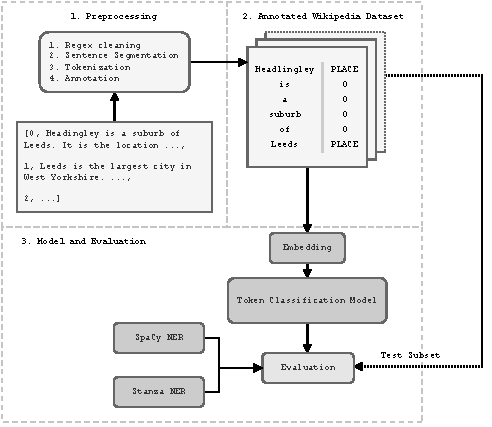
\includegraphics[width=0.8\textwidth,height=\textheight]{03_transformer/./03_figures/figure1.pdf}

}

\caption{\label{fig-workflow}Overview of the model processing pipeline}

\end{figure}

\hypertarget{software-hardware-infrastructure}{%
\subsection{Software \& hardware
infrastructure}\label{software-hardware-infrastructure}}

Models used in our paper were written in
\href{https://www.python.org/}{\texttt{Python}} using the
\href{https://allennlp.org/}{\texttt{AllenNLP}} library for deep
learning in natural language processing (Gardner \emph{et al.}, 2018).
\texttt{AllenNLP} is built on top of
\href{https://pytorch.org}{\texttt{PyTorch}} (Paszke \emph{et al.},
2019), providing abstractions to commonly used operations for working
with state-of-the-art deep neural networks in natural language
processing.

Model training was GPU accelerated using a single NVIDIA GeForce RTX
2070 SUPER with 8192MB memory paired with a Ryzen 3700x CPU with 8
physical and 16 logical cores. \texttt{Python} version 3.8.5 was used
with \texttt{AllenNLP} version 1.5.0.

\hypertarget{annotation-data-collection}{%
\subsection{Annotation \& data
collection}\label{annotation-data-collection}}

\hypertarget{wikipedia-data-collection}{%
\subsubsection{Wikipedia data
collection}\label{wikipedia-data-collection}}

Wikipedia presents a large collection of well-formatted text contributed
by a variety of users, with frequent instances of place names, a
consistent written style and without misspellings. Existing NER models
are trained on either CoNLL-03 or OntoNotes 5, both of which are
well-formatted text datasets, consisting primarily of news articles. As
such, it was considered appropriate to select Wikipedia for a comparison
between these models and ours, compared with other sources of VGI that
are of lower overall quality.

The Wikipedia text data used in our paper was accessed through
\href{https://wiki.dbpedia.org/}{DBpedia} (Auer \emph{et al.}, 2007), a
community gathered database of information from Wikipedia, presented as
an open knowledge graph, with ontologies that link and define
information in articles. A query was built to obtain English Wikipedia
abstracts for each DBpedia article with the \texttt{Place} class in
Great Britain, using the \href{http://dbpedia.org/sparql}{DBpedia SPARQL
endpoint}. Querying just for \texttt{Place} articles within Great
Britain ensured that articles extracted contained a large number of
place names and language indicative of place names, without additional,
unnecessary information.

These abstracts are the text provided at the top of each article, before
any headings, sometimes called the summary. As an example, the Wikipedia
abstract for \href{https://en.wikipedia.org/wiki/Rowlatts_Hill}{Rowlatts
Hill}, a suburb of Leicester, UK is as follows, with hyperlinks
indicated in bold:

\begin{quote}
Rowlatts Hill (also known as Rowlatts Hill Estate, or R.H.E.) is an
eastern, residential suburb of the \textbf{English} city of
\textbf{Leicester}. It contains mostly \textbf{council-owned housing}.
\end{quote}

\begin{quote}
The suburb is roughly bordered by Spencefield Lane to the east and
Whitehall Road to the south, which separates it from neighbouring
\textbf{Evington}. A second boundary within the estate consists of
Coleman Road to Ambassador Road through to Green Lane Road; Rowlatts
Hill borders \textbf{Crown Hills} to the west. To the north, at the
bottom of Rowlatts Hill is Humberstone Park which is located within
Green Lane Road, Ambassador Road and also leads on to Uppingham Road
(the \textbf{A47}), which is also Rowlatts Hill.
\end{quote}

Using DBpedia enabled a fast executing query which, when combined with
the \texttt{Place} class from the DBpedia ontology, returned a complete
dataset of Wikipedia pages for many geographic locations in Great
Britain. A total 42,222 article abstracts were extracted.

\hypertarget{input-format}{%
\subsubsection{Input format}\label{input-format}}

For use in the models, a random subset of 200 articles were annotated
using the CoNLL-03 NER format, which uses line delimitation to separate
tokens, with entities associated with each token sharing the same line,
separated by a space. Articles were first cleaned using regular
expressions to remove quotation marks, text inside parentheses, and
non-ascii characters. The \texttt{SpaCy} large web-based pre-trained
model pipeline (\texttt{en\_core\_web\_lg}) was used for further
processing, using a non-monotonic arc-eager transition-system for
sentence segmentation (Honnibal and Johnson, 2015), and tokenisation
using a rule-based algorithm. Each sentence-length sequence of tokens
was treated as a separate instance to be fed as batches into models for
training. Each token in every sequence was annotated as being a place
name or not, assisted through the open source annotation tool
\href{https://github.com/doccano/doccano}{Doccano} (Nakayama \emph{et
al.}, 2018).

For place names that span multiple tokens, the \emph{BIOUL} tagging
scheme was used, which stands for the `\emph{\textbf{B}eginning},
\emph{\textbf{I}nside} and \emph{\textbf{L}ast} tokens of multi-token
chunks'; for place names that span more than one token
(e.g.~\emph{B-Place}: New, \emph{L-Place}: York).
`\emph{\textbf{U}nit-length} chunks and \emph{\textbf{O}utside}', place
names of only a single token, and outside for any token that isn't a
place name. This scheme was used over the simpler BIO scheme which is
more difficult for models to learn (Ratinov and Roth, 2009). During
annotation it became clear that the length of certain multi-token place
names could be considered ambiguous. For example, it may not be clear
when a cardinal direction is part of a place name, `northern Ireland'
may refer to a northern region in Ireland, while `Northern Ireland'
refers to the constituent country in the United Kingdom. To unify
labelling decisions we chose to consider capitalisation as an indication
of multi-token noun phrases that constituted a single place name. The
following sentence shows a sequence of tokens with their corresponding
tags, demonstrating the annotation scheme with \emph{BIOUL} information
prepending each tag:

\begin{figure}[H]
\centering
\begin{dependency}
\tikzstyle{word}=[font=\normalsize]
\tikzstyle{tag}=[font=\bfseries\tiny]
\begin{deptext}[column sep=0.05cm, row sep=0.1cm]
\& |[word]| \textit{Kingston} \& |[word]| \textit{upon} \& |[word]| \textit{Hull} \& |[word]| is
\& |[word]| usually \& |[word]| abbreviated  \& |[word]| to \& |[word]| \textit{Hull} \\
\& |[tag]| B-PLACE \& |[tag]| I-PLACE \& |[tag]| L-PLACE \& |[tag]| O
\& |[tag]| O \& |[tag]| O \& |[tag]| O \& |[tag]| U-PLACE \\
\end{deptext}
\end{dependency}
\end{figure}

From these 200 labelled Wikipedia abstracts, 10\% were kept for both
validation and testing, leading to a training set of 21,080 labelled
tokens, a validation dataset of 2,907 labelled tokens, and a testing
dataset of 3,347 labelled tokens.

\hypertarget{building-the-entity-recognition-models}{%
\subsection{Building the entity recognition
models}\label{building-the-entity-recognition-models}}

Named entity recognition is a subset of token classification where a
sequence of tokens \(\mathbf{x} = \{x_{0}, x_{1}\dots x_{n}\}\) are
taken as input, and the most likely sequence tags
\(\mathbf{y} = \{y_0, y_1, \dots y_n\}\) are predicted. The models
constructed in our paper may be divided into three main components,
outlined on Figure \ref{fig-workflow}:

\begin{itemize}
\tightlist
\item
  \textbf{Embedding Layer}: Each token in a sequence represented as high
  dimension numerical space, they may be either:

  \begin{itemize}
  \tightlist
  \item
    Randomly initialised
  \item
    Pre-trained: GloVe, transformer
  \end{itemize}
\item
  \textbf{Intermediate Layers:} A deep neural network that input
  embeddings propagate through, either:

  \begin{itemize}
  \tightlist
  \item
    Bidirectional LSTM
  \item
    Transformer
  \end{itemize}
\item
  \textbf{Classification layer:} The final layer of the model that takes
  a high dimensional output from the previous layers, and projects them
  to the classification dimension. The \texttt{argmax} from this layer
  corresponds to the label selected for each token. Each model uses a
  Conditional Random Field (CRF) to classify tokens which are popular in
  NER tasks, as they consider tagging decisions between all input tokens
  (Lample \emph{et al.}, 2016). This is necessary given the inside tag
  for a place (I-PLACE), cannot directly follow a unit tag (U-PLACE) for
  example.
\end{itemize}

\begin{table}
\caption{\label{tbl-models}Overview of the models trained through our paper, detailing the architecture used. Integers in brackets indicate the vector dimensions}
\centering
\fontsize{9}{11}\selectfont
\begin{tabular}[h]{lllll}
\toprule
\textbf{Name} & \textbf{Embeddings} & \textbf{Intermediate} & \textbf{Output} & \textbf{Optimiser}\\
\midrule
\texttt{BiLSTM-CRF (Basic)} & Token \{50\} & 2-layer BiLSTM \{200\} & CRF & Adam\\
\texttt{BiLSTM-CRF} & \makecell[l]{GloVe Token \{50\}\\ Character \{16\}} & 2-layer BiLSTM \{200\} & CRF & Adam\\
\texttt{BERT} & BERT \{768\} & 12-layer Transformer \{768\} & CRF & AdamW\\
\texttt{RoBERTa} & RoBERTa \{768\} & 12-layer Transformer \{768\} & CRF & AdamW\\
\texttt{DistilBERT} & DistilBERT \{768\} & 6-layer Transformer \{768\} & CRF & AdamW\\
\bottomrule
\end{tabular}
\end{table}

Table \ref{tbl-models} gives an overview of the model architectures
built through our paper. First a simplistic model was constructed as a
baseline, using untrained randomly initialised 50 dimension token
embeddings, fed into a two-layer Bidirectional LSTM (BiLSTM) with 200
hidden dimensions. The output from the BiLSTM was input into a
conditional random field classifier. A second BiLSTM model was also
created based on the architecture described in Peters \emph{et al.}
(2018), adding pre-trained GloVe token embeddings (Pennington, Socher
and Manning, 2014) with 50 dimensions and 16 dimension character
embeddings. Both models used the \texttt{Adam} optimiser which makes use
of stochastic gradient descent for weight optimisation (Kingma and Ba,
2017).

Three BERT-based transformer models were also created, using BERT
(Devlin \emph{et al.}, 2019), RoBERTa which attempts to optimise the
training process of BERT (Liu \emph{et al.}, 2019), and DistilBERT,
which distils the data used in pre-training to create a smaller, faster
model (Sanh \emph{et al.}, 2020). The primary architecture of
transformers is `attention' which enables them to consider and weight
each word in a sequence against each other word simultaneously. This
allows them to be highly parallel, providing significant improvements to
computational speed with GPUs which can handle highly parallel tasks,
and benefits over traditional architectures like Long Short-Term Memory
(LSTM) which are only able to consider sequences sequentially (Vaswani
\emph{et al.}, 2017). These models were pre-trained on very large
general text corpora, enabling `transfer learning', where a pre-trained
model like BERT is used as a base and fine-tuned to be task specific.
Conceptually, these pre-trained models learn deep embedded weights for
words based on comprehensive contextual information extracted from the
large general text corpora, these then only require smaller adjustments
in fine-tuning to achieve good task-specific results. Fine-tuning these
pre-trained models in NLP has produced results that often outperform
models using traditional architectures that include manually trained
word embeddings (Word2Vec, Mikolov \emph{et al.}, 2013), which are
limited by the volume of data provided to them and pre-trained
embeddings like GloVe (Pennington, Socher and Manning, 2014).

Pre-trained transformer models replace both the BiLSTM layers of the
previous models and token embeddings, taking encoded sequences,
associating each token with a 768 dimension vector representation from a
vocabulary, feeding them into sequential transformer layers and
outputting into a CRF classifier. Each model was initialised with
pre-trained weights provided by the \texttt{transformers} Python library
(Wolf \emph{et al.}, 2020), these weights are initialised in both the
embedding layers and intermediate layers. For weight optimisation, these
models used the weight decay Adam algorithm (\texttt{AdamW}, Loshchilov
and Hutter, 2019). Every layer of the transformer models was updated
during training, which enabled the pre-trained weights to adjust and
learn for the specific task. Hyper-parameters selected for each model
were largely based on the values as suggested for token classification
by their respective implementation papers.

For every model, weights were adjusted each epoch to minimise the
training loss. Following the final intermediate layer of a model, a
token representation \(C\in\mathbb{R}^H\) feeds into the classification
layer weights \(W\in\mathbb{R}^{K\times H}\), where \(K\) is the number
of unique labels. Classification loss is then calculated using
\(log(softmax(CW^T))\).

Early stopping was used in each model, stopping training early if no
improvement was made to the validation F\textsubscript{1} score in eight
subsequent epochs. Automatic Mixed Precision (AMP) was used throughout
training to use half-precision (16 bit) floating point numbers in some
operations which reduced the memory overhead and increased computation
speed. For transformers, the learning rate was optimised towards the end
of training, using a \texttt{reduce\ on\ plateau} learning rate
scheduler, reducing the learning rate by 1/10th once the overall
F\textsubscript{1} validation metric had stopped improving after two
epochs, this only increased training time on the BiLSTM models with no
improvement, so was excluded. Following training, the weights from the
best performing epoch were automatically chosen for the final model.

\hypertarget{evaluation-against-pre-built-models}{%
\subsection{Evaluation against pre-built
models}\label{evaluation-against-pre-built-models}}

Following the training of each model, their accuracy, precision, recall
and F\textsubscript{1} score was evaluated using a corpus of test data,
against three popular modern pre-built NER models provided through the
\texttt{SpaCy} and \texttt{Stanza} Python packages. A \texttt{SpaCy}
model is used in the \emph{Mordecai} geoparser and optionally in the
\emph{GeoTxt} geoparser, while the \texttt{Stanza} model is a more
recent implementation of the Stanford NLP model used by the
\emph{GeoTxt} geoparser.

As these pre-built models were not trained to recognise `place names',
their tags were adjusted so that anything labelled as `GPE'
(Geopolitical Entity), `LOC' (Location), or `FAC' (facility) was
considered to be a `place name', mirroring the process used to discard
unrelated entities by geoparsing systems that use these models. The
default \texttt{Stanza} NER model, and two \texttt{SpaCy} models
(\texttt{en\_core\_web\_sm}, \texttt{en\_core\_web\_lg}) were evaluated
on the labelled test data. Table \ref{tbl-prebuilt} gives an overview of
these pre-built models.

Each model was evaluated on 3 separate subsets of the annotated test
dataset, giving a range of scores for each model. Significance testing
was then performed using paired t-tests to test the null hypothesis:

\begin{quote}
\(\mathbf{H_0}\): There will be no statistically significant difference
between the mean F\textsubscript{1} score of each custom built model
against the best performing pre-built model (\texttt{Stanza}).
\end{quote}

Significant results that reject this null hypothesis were indicated by
\(p<0.05\) and are shown on Table \ref{tbl-eval}.

The best performing model trained on the annotated Wikipedia data was
also evaluated using paired t-tests against each other model trained on
the same data, to test the null hypothesis:

\begin{quote}
\(\mathbf{H_0}\): There will be no statistically significant difference
between the mean F\textsubscript{1} score of the best performing custom
built model trained on annotated Wikipedia data and each other model
trained on this data.
\end{quote}

Significant results that reject this null hypothesis were also indicated
by \(p<0.05\).

It should be noted that significance testing is not common in deep
learning research (Dror and Reichart, 2018), but papers that do report
the significance of mean scores between models tend to use paired
t-tests, despite potentially violating the parametric assumptions made.
Dror and Reichart (2018) suggest that while normality may be assumed due
to the Central Limit Theorem, it is likely that future progress in this
field will present more appropriate statistical significance testing.

\begin{table}

\caption{\label{tbl-prebuilt}Pre-built NER models}
\centering
\fontsize{9}{11}\selectfont
\begin{tabular}[t]{lllc}
\toprule
\textbf{Name} & \textbf{Training Data} & \textbf{Architecture} & \textbf{Reported NER $F_{1}$}\\
\midrule
SpaCy (small) & OntoNotes 5 & CNN & 0.84$^a$\\
SpaCy (large) & OntoNotes 5 & CNN & 0.85$^a$\\
Stanza & OntoNotes 5 & BiLSTM CRF & 0.89$^b$\\
\bottomrule
\multicolumn{4}{l}{\rule{0pt}{1em}a \href{https://spacy.io/models/en}{https://spacy.io/models/en}}\\
\multicolumn{4}{l}{\rule{0pt}{1em}b \href{https://stanfordnlp.github.io/stanza/performance.html}{https://stanfordnlp.github.io/stanza/performance.html}}\\
\end{tabular}
\end{table}

\hypertarget{output-processing}{%
\subsection{Output processing}\label{output-processing}}

A predictor was created from the DistilBERT model to run inference over
the total corpus of Wikipedia articles. Place names extracted from the
Wikipedia articles by this model were saved to a CSV file with the
context sentence, the associated article, and coordinate information for
the article that contained the place.

Place names were compared against a full corpus of British place names
from the GeoNames gazetteer, to examine which names are excluded from
the gazetteer, but identified within Wikipedia articles.

\hypertarget{sec-trans-results-discussion}{%
\section{Results \& discussion}\label{sec-trans-results-discussion}}

This section first evaluates the results of the models presented against
each other, and in relation to existing pre-built NER solutions. The
place names extracted by our best performing model are compared with
pre-built models, showing how our method improves on those used in
existing place name extraction methods. Following this, examples from
the corpus of place names extracted from Wikipedia articles are noted,
demonstrating use-cases for the method presented that wouldn't be
possible or as effective, through pre-built NER solutions.

\hypertarget{model-performance}{%
\subsection{Model performance}\label{model-performance}}

Table \ref{tbl-eval} shows three popular pre-built NER models, evaluated
on the labelled Wikipedia test data, compared with the models produced
through our paper. The \texttt{BiLSTM-CRF\ (basic)} model gives a
baseline reference for a typical NER model with a simple architecture.
Out of the pre-built models, \texttt{Stanza} performs the best,
achieving precision and accuracy just below the trained baseline model,
with an F\textsubscript{1} score which isn't significantly worse (paired
t-test \(p>0.05\)), both \texttt{SpaCy} models however show notably
worse results compared with \texttt{Stanza}. The primary issue with the
pre-built models is recall, which is far below any of the custom-built
models, reflecting a high number of false negatives.

\begin{table}

\caption{\label{tbl-eval}Geographic entity recognition mean (±SD) performance metrics over 3 runs of annotated Wikipedia test data subsets. Pre-built NER models are shown in italics. Bold values indicate statistically significant F1 scores of fine-tuned models in relation to `Stanza` (Paired t-tests $p<0.05$).}
\centering
\fontsize{9}{11}\selectfont
\begin{tabular}[t]{llccc}
\toprule
\textbf{ } & \textbf{Accuracy} & \textbf{Precision} & \textbf{Recall} & \textbf{F1}\\
\midrule
BERT & 0.985 ±0.0050 & 0.947 ±0.0241 & 0.932 ±0.038 & \textbf{0.939 ±0.0256}\\
DistilBERT & 0.980 ±0.0015 & 0.930 ±0.0065 & 0.918 ±0.015 & \textbf{0.924 ±0.0065}\\
RoBERTa & 0.982 ±0.0055 & 0.916 ±0.0069 & 0.931 ±0.015 & \textbf{0.923 ±0.0086}\\
CRF biLSTM & 0.967 ±0.0068 & 0.909 ±0.0104 & 0.813 ±0.017 & 0.859 ±0.0124\\
CRF biLSTM (basic) & 0.947 ±0.0040 & 0.836 ±0.0546 & 0.698 ±0.023 & 0.760 ±0.0135\\
\midrule
\em{Stanza} & \em{0.941 ±0.0259} & \em{0.757 ±0.0542} & \em{0.705 ±0.068} & \em{0.730 ±0.0586}\\
\em{SpaCy (Large)} & \em{0.910 ±0.0191} & \em{0.724 ±0.0422} & \em{0.451 ±0.050} & \em{0.554 ±0.0382}\\
\em{SpaCy (small)} & \em{0.900 ±0.0225} & \em{0.720 ±0.0594} & \em{0.345 ±0.082} & \em{0.464 ±0.0835}\\
\bottomrule
\end{tabular}
\end{table}

It is worth noting that due to class imbalances, i.e.~many more `other'
(\texttt{O}) entities relative to the small number of \texttt{PLACE}
entities, accuracy should be considered a poor metric, and is only
included for completeness. This class imbalance means that as only
approximately 15\% of tokens are labelled as entities, it is possible to
achieve 85\% accuracy and high precision by labelling all tokens as not
entities. F\textsubscript{1} score is often used to compensate for these
issues in multiple classification tasks, but it should be known that it
is not itself a perfect metric. With respect to the best performing
pre-built model \texttt{Stanza}, all transformer models fine-tuned on
the Wikipedia annotated data, have significantly higher
F\textsubscript{1} scores (paired t-test \(p<0.05\)).

The DistilBERT transformer model is less complex than both the BERT and
RoBERTa model, with a total of 260 MB in model weights, compared with
433 MB and 498 MB respectively. Despite this, the DistilBERT model
achieves similar results to RoBERTa on test data (Table \ref{tbl-eval}).
While all transformer models perform significantly better than the best
performing pre-built model, Stanza, both CRF models do not give
significantly better F\textsubscript{1} scores (paired t-test
\(p>0.05\)). BERT performs best overall, with an F\textsubscript{1}
score of 0.939 on the test data, a result that is only significantly
better than the two CRF models (paired t-test \(p<0.05)\).

Figure \ref{fig-qual} shows the output of the chosen fine-tuned NER
model \texttt{DistilBERT} alongside \texttt{SpaCy\ (large)} and
\texttt{Stanza}, applied to a simple Wikipedia article summary. Figure
\ref{fig-qual} (A) gives promising results for \texttt{DistilBERT}, with
the summary for the Wikipedia page `Rowlatts Hill', correctly
identifying all place names.

While evaluation metrics indicate that \texttt{Stanza} performs
reasonably well, it primarily suffers from the annotation scheme used,
some place names are misidentified as `Person', or `Organisation',
meaning a standard geoparsing system would miss several place names
here, given they are not otherwise identifiable (Figure \ref{fig-qual}).

\begin{figure}

{\centering \includegraphics{03_transformer/./03_figures/figure2.jpg}

}

\caption{\label{fig-qual}Comparison of outputs between the best
performing fine-tuned transformer model and the two best performing
pre-built NER models.}

\end{figure}

\begin{figure}

{\centering \includegraphics{03_transformer/./03_figures/figure3.jpg}

}

\caption{\label{fig-qual-china}Ability for trained model to distinguish
between metonymic usage of place names.}

\end{figure}

Figure \ref{fig-qual-china} demonstrates the ability for our DistilBERT
transformer model to accurately ignore entities that do not relate to
place names. This example paragraph only refers to a single geographic
location in text, the location of the 1952 Summer Games, in Helsinki,
Finland. While Stanza identifies a large number of GPE tags, they either
relate to China used in a metynomic sense, meaning the Chinese Olympic
team (`China competed'), or as a related geopolitical noun (`delegation
of ROC'), which is not considered to be a place name referring to a
geographic location in this context. Our model correctly infers the
single mention of a geographic place name based on the contextual
information, meaning a large amount of unrelated information is
excluded. Particularly, recognising and ignoring these nouns related to
place names is something that is noted as an issue in current geoparsing
systems (Gritta, Pilehvar and Collier, 2020). This figure also
demonstrates the importance of using a pre-trained model base for this
task, as the BiLSTM CRF performs poorly. It is likely that this issue
stems from the limited training data used, as the model is unable to
learn more complex cases where place names are less obvious (Figure
\ref{fig-qual-china} (B)). Using a pre-trained transformer enables the
model to correctly identify instances where proper nouns do not relate
to place names, taking information learned through its pre-training
procedure.

\hypertarget{identified-place-names-from-wikipedia}{%
\subsection{Identified place names from
Wikipedia}\label{identified-place-names-from-wikipedia}}

\begin{table}
\caption{\label{tbl-freq}Top and bottom named places by frequency, excluding any present in the GeoNames gazetter or mentioned less than 100 times.}

\centering
\fontsize{9}{11}\selectfont
\begin{tabular}[t]{lll}
\toprule
\bfseries IDX & \bfseries Place (DistilBERT) & \bfseries Count\\
\midrule
70 & Great Western Railway & 236\\
77 & Ceredigion & 220\\
78 & West Riding of Yorkshire & 217\\
79 & East Lindsey & 217\\
83 & Midland Railway & 212\\
87 & London Underground & 195\\
... & ... & ...\\
176 & M4 & 108\\
180 & North Norfolk & 106\\
181 & M1 & 106\\
182 & Church of England & 106\\
191 & Hull & 104\\
199 & Great Northern Railway & 101\\
\bottomrule
\end{tabular}
\centering
\begin{tabular}[t]{lll}
\toprule
\bfseries IDX & \bfseries Place (SpaCy) & \bfseries Count\\
\midrule
3 & the United Kingdom & 458\\
4 & Tyne & 353\\
5 & Ceredigion & 282\\
6 & the City of London & 211\\
7 & Methodist & 205\\
8 & the Metropolitan Borough of & 200\\
... & ... & ...\\
14 & France & 129\\
15 & Baptist & 127\\
16 & Sutherland & 119\\
17 & the City of & 116\\
18 & Richmondshire & 109\\
19 & Thameslink & 102\\
\bottomrule
\end{tabular}
\end{table}

Table \ref{tbl-freq} gives an overview of the most common place names
identified by the DistilBERT model and the SpaCy model. Notably, the
SpaCy model appears to struggle with correctly aligning entities,
including `the' with `United Kingdom', and partially missing place names
containing `Tyne' (e.g.~`Tyne and Wear' or `River Tyne'). The DistilBERT
model also extracts around 6 times the number of place names compared
with SpaCy, reflected by the low recall noted above. One example where
the DistilBERT model appears confused is by giving the place name
`Church of England', this problem relates to the language used in
Wikipedia articles, when churches are described as a `Church of England
church', a nominal mention of a place rather than specific.

The total number of place names extracted from the Wikipedia summaries
by the \texttt{DistilBERT} model was 614,672, with 99,697 unique place
names. In total 62,178 unique place names were extracted that are not
found within the GeoNames gazetteer. These entities primarily exist as
granular names mentioned in single instances (e.g.~road names: Shady
Lane, Chapeltown Road), organisational names used in a place related
context (e.g.~describing locations along the Great Western Railway
route), and alternative names that are not captured by GeoNames. For
example, `M1' appears in GeoNames as `M1 Motorway'\footnote{https://www.geonames.org/8714914/m1-motorway.html}.
While the `M1 motorway' is used in Wikipedia articles, it is often also
referred to as just the `M1'.

\hypertarget{conclusion}{%
\section{Conclusion}\label{conclusion}}

Our paper demonstrates a new approach towards the extraction of place
names from text by building an NER model using data annotated with
geographic place names. This work aims to direct geographic NLP research
towards the use of models which move away from the generalisable
annotation schemes of pre-built NER solutions, to include task-specific,
relevant training data. Notably this differs from the perceived
generalisability of pre-built models used for general geoparsing. We
believe this is an important approach for geographic place name
extraction given geographic language differs greatly based on context
(Purves \emph{et al.}, 2018), with contexts varying greatly based on the
corpora used for inference. This is demonstrated by the poor results
observed in previous work when applying pre-built NER solutions, which
use training data unrelated to the task-specific data they are being
applied to (Hu, Mao and McKenzie, 2019; Karimzadeh \emph{et al.}, 2019).
Wallgrün \emph{et al.} (2018) recognise this problem, developing
GeoCorpora, a task-specific training dataset for micro-blog geoparsing,
notably describing increased issues with annotation ambiguity compared
with more traditional text-sources. Additionally, recent work with
transformer models, typically only built to be generalisable, have
considered moving from fully generalised self-supervised training
towards more dataset-specific models (e.g.~TweetEval; Barbieri \emph{et
al.} (2020)), with results that outperform generalisable transformer
models (Nguyen, Vu and Nguyen, 2020).

Ultimately, the decision to produce a model explicitly designed to be
non-generalisable to other corpora may be considered a limitation of the
scope of this paper. We have demonstrated a best-case scenario where
time-frames allow for manual annotation of task-specific data. Future
research may consider the construction of a more generalisable place
name extraction model, which takes inspiration from the alternative
annotation scheme employed by our paper, allowing for use in general
purpose geoparsers.

Additionally, while our paper selects Wikipedia for place name
extraction, due to its large volume, ease of validation and data
retrieval, future work may consider the ability to apply our methodology
to other text sources. With suitable models constructed, using annotated
training data that is relevant to the corpus being considered, we expect
future work applied to other data sources may present the opportunity to
further contribute to place names that are absent from gazetteers, as
vernacular place names. We believe that given a suitable combination of
data sources, our methodology is the first step towards the construction
gazetteers from the bottom-up, directly taking place names from passive
contributions, without relying on pre-built datasets.

The recent development of pre-trained language models and their
suitability for fine-tuning in many tasks, including NER, presents a
method for the construction of accurate models that are task specific,
using relatively small labelled corpora\footnote{Compared with the
  Reuters corpus used for CoNLL03 for example} that defines entities
more suited to the task of place name extraction. The architecture in
our paper is more simplistic to implement than other attempts at similar
tasks (e.g. Weissenbacher \emph{et al.}, 2019), with most of the
complexity hidden within the transformer layers. This, combined with
libraries that abstract and implement state of the art models, provides
a more accessible approach for research in place name extraction,
without requiring a deep understanding of semantic rules, or the
construction of deep multi-layered models from the ground up.

Evaluation against pre-built NER models on Table \ref{tbl-eval} shows
that performance for place name extraction is greatly improved,
particularly with respect to recall, a notable issue with past studies
(Hu, Mao and McKenzie, 2019; Karimzadeh \emph{et al.}, 2019). The
construction of an NER model for the task specific extraction of place
names moves towards systems that appropriately consider the geographic
elements present in natural language. The large number of place names
that are absent from the GeoNames gazetteer suggests that geoparsing and
related work likely misses a substantial amount of geographic
information present in text. The dataset produced through this work aims
to assist with filling these gaps, while the methodology described
enables an approach that may be mirrored and applied to further work on
other data sources.

Finally, both `place' focussed annotation schemes describe the use of
`nominal' place related entities (Mani \emph{et al.}, 2010; Pustejovsky,
2017). While out of the scope of our work, we would like to encourage
the focus on extracting this additional geographic information from
text. Often in language the use of these non-specific terms are used,
for example `I visited the shops', `York is a city', provide
geographically specific information. `The shops' with enough context may
provide a specific geographic location, and similarly the link between
`York' -\textgreater{} `city' could be explored (Couclelis, 2010).

\hypertarget{data-and-codes-availability-statement}{%
\section*{Data and codes availability
statement}\label{data-and-codes-availability-statement}}
\addcontentsline{toc}{section}{Data and codes availability statement}

\markright{Data and codes availability statement}

The data and codes that support the findings of this study are available
at the public FigShare link
(\url{https://doi.org/10.6084/m9.figshare.13415255.v1}). Instructions
for using the data and code are provided as a README within the FigShare
repository.

\hypertarget{disclosure-statement}{%
\section*{Disclosure statement}\label{disclosure-statement}}
\addcontentsline{toc}{section}{Disclosure statement}

\markright{Disclosure statement}

No potential competing interest was reported by the authors.

\bookmarksetup{startatroot}

\hypertarget{sec-connections}{%
\chapter{Mapping Cognitive Place Associations within the United Kingdom
through Online Discussion on Reddit}\label{sec-connections}}

\chaptermark{Mapping Cognitive Place Associations within the United Kingdom}

\textbf{The content of this chapter is \emph{under review} for
publication in \emph{Transactions of the Institute of British
Geographers}.}

\hypertarget{chapter-overview-1}{%
\subsection*{Chapter Overview}\label{chapter-overview-1}}
\addcontentsline{toc}{subsection}{Chapter Overview}

To achieve the second aim of this thesis, this chapter considers the
ability to extract place-based geographic knowledge from comments on the
social media website Reddit. By implementing the geoparsing methodology
outlined in Chapter~\ref{sec-transformer}, a large volume of place names
are identified in these comments, and associated with coordinate
information, using the OS Open Names gazetteer. `Cognitive place
associations' are generated from these locational mentions, presenting a
formalisation of subconscious links between locations that form through
the mental maps of individuals in this corpus. To explore the geographic
properties of these associations, this chapter generates a measure of
distance decay using a gravity model.

\hypertarget{abstract-2}{%
\subsection*{Abstract}\label{abstract-2}}
\addcontentsline{toc}{subsection}{Abstract}

This paper explores cognitive place associations; conceptualised as a
place-based mental model that derives subconscious links between
geographic locations. Utilising a large corpus of online discussion data
from the social media website Reddit, we experiment on the extraction of
such geographic knowledge from unstructured text. First we construct a
system to identify place names found in Reddit comments, disambiguating
each to a set of coordinates where possible. Following this, we build a
collective picture of cognitive place associations in the United
Kingdom, linking locations that co-occur in user comments and evaluating
the effect of distance on the strength of these associations. Exploring
these geographies nationally, associations were shown to be typically
weaker over greater distances. This distance decay is also highly
regional, rural areas typically have greater levels of distance decay,
particularly in Wales and Scotland. When comparing major cities across
the UK, we observe distinct distance decay patterns, influenced
primarily by proximity to other cities.

\hypertarget{sec-introduction}{%
\section{Introduction}\label{sec-introduction}}

The importance of relational thinking to understand geographical
phenomena has been widely acknowledged in human and computational
geography (Lukermann, 1961; Bergmann and O'Sullivan, 2018; Glückler and
Panitz, 2021). Spatial networks have been explored from a variety of
perspectives, to uncover the dynamics underpinning the spatial
behaviours of individuals (González, Hidalgo and Barabási, 2008; Noulas
\emph{et al.}, 2011), or to challenge conceptualisations of regions as
bounded by administrative definitions (Alessandretti, Aslak and Lehmann,
2020; Calafiore \emph{et al.}, 2021).

Within computational geography, most research has explored direct
connections between places by investigating physical movements of
individuals, using population movement data from both traditional data
sources such as Census or surveys (Rae, 2009; Titheridge \emph{et al.},
2009), or through alternative forms of data like transport records
(Farber and Li, 2013; Allard and Moura, 2016; Yang, Li and Li, 2019;
Gong \emph{et al.}, 2021), mobile phone data (Lin, Wu and Li, 2019;
SafeGraph, 2022; Rowe \emph{et al.}, 2022), and geotagged social media
(Steiger \emph{et al.}, 2015; Ostermann \emph{et al.}, 2015; Arthur and
Williams, 2019; Li \emph{et al.}, 2021). However, focussing only on
connections built through population movement conceals associations that
persist through individuals or community subconscious, regardless of any
physical movement.

Literature discussing the role of human cognition in constructing mental
images of cities (Lynch, 1964), and how they can be represented through
mental maps (Gould and White, 1986), reveals that the way humans
conceive spatial structures and associations between places are
substantially entrenched in individuals' experiences and geographic
knowledge, which only partially derive from movements. Places represent
a complex network of socio-spatial relationships that emerge from linked
individual experiences (Pierce, Martin and Murphy, 2011), enabling the
definition of collectively recognised place associations. While
movements in geographic space are limited by time and distance
(Patterson and Farber, 2015; Miller, 2018), representational spaces
expressed through mental maps are not necessarily bounded by
spatio-temporal constraints (Merrifield, 1993). Modern developments in
transport and communication access warp the perceptions of distance
between places (Massey, 2008), and in turn their perceived level of
connectivity (Fabrikant \emph{et al.}, 2002).

Alternatively, online sources of data offer novel opportunities to
explore place associations, built directly from the passive
contributions of individual users. Recent work has demonstrated how
digital social friendships (Bailey \emph{et al.}, 2018), or embedded
links in Wikipedia articles (Salvini and Fabrikant, 2016), may be used
to provide insight into social place connections. Other works have
instead considered that text itself can be used to quantify
relationships between geographic terms, described as `geo-semantic
relatedness' (Ballatore, Bertolotto and Wilson, 2014). Work building on
this concept has applied it to city and region names identified in news
articles, social media, and general web pages (Liu \emph{et al.}, 2014;
Hu, Ye and Shaw, 2017; Meijers and Peris, 2019; Ye, Gong and Li, 2021).

Distance is a key influence on observed levels of connectivity in
spatial interaction literature (Haynes and Fotheringham, 1985), and
Tobler's first law of geography, where locations that are further apart
are typically less well-connected (Tobler, 1970), has generated the term
`distance decay' (Taylor, 1983), which has various forms of mathematical
representation. Given a legacy of empirical evidence, distance decay in
its various forms can be sensibly assumed in place connections when both
temporal and spatial constraints are considered in our physical
environment. However, when considering the links between locations from
the perspective of cognitive associations built through mental maps,
such constraints are no longer as restrictive (Fabrikant \emph{et al.},
2002). Quantifying the effect of distance on cognitive place
associations may therefore result in unexpected patterns in the effect
of distance on associations, that reveal the cognitive biases used to
construct mental maps.

The objective of this paper is to quantify cognitive place associations
across the UK\footnote{Ordnance Survey UK does not include data for
  Northern Ireland.} to build mental maps, while evaluating the effect
of distance on the strength of these associations, measuring the level
of distance decay through a gravity model. To generate association
measures from a cognitive rather than geographic perspective, we infer
associations through co-occurring locations extracted from a large
corpus of informal, unstructured and discursive text from the social
media website Reddit. Locations when mentioned in informal comments are
drawn from a cognitive process associated with mental maps of these
locations, subconsciously illustrating associations between places from
memory and based on experience.

Section~\ref{sec-cognitive-place-associations} outlines existing
literature relating to cognitive place associations, detailing methods
that can be used for the automated extraction and grounding of place
names\footnote{In our work we consider `place names' to be ambiguous
  noun phrases found in text, without associated coordinates, while
  `locations' are place names that have attributed coordinates. We use
  `\emph{place} associations' to capture the vagueness involved in
  cognitive associations.} from a large corpus of unstructured text.
Section~\ref{sec-methodologycon} provides details on our data sources,
our methodology for geoparsing place names, and the computation of a
gravity model to examine the effects of distance decay on the strength
of associations. In Section~\ref{sec-resultscon} we present the results
of our gravity model and demonstrate variations in distance decay with
respect to six locations. In Section~\ref{sec-conclusioncon} we conclude
our findings and outline the scope for future work.

\hypertarget{sec-cognitive-place-associations}{%
\section{Cognitive Place
Associations}\label{sec-cognitive-place-associations}}

The term `mental map' typically refers to the cognitive visualisation of
a geographic environment. They represent collective, experiential
geographic knowledge, relating to both places, and the relationships
between them (Kaplan, 1976). Mental maps exhibit a variety of biases,
for example, they are often more detailed with respect to locations that
we are familiar with, while others may be less detailed or even absent
entirely (Gould and White, 1986). The scale and distance between
features in mental maps can be warped (Peake and Moore, 2004; Marston,
Jones III and Woodward, 2005); prominent roads may appear larger than in
reality, skyline features in a city may be perceived as less prominent
due to their irrelevance to an individual at street level (Lynch, 1964;
Gould and White, 1986), and good transport connections narrow the time
it takes to reach connected locations, which in turn reduces the
perceived distance between them (Merrifield, 1993; Massey, 2008).
Intermediate features along common routes also have varying levels of
importance to individuals; unimportant features may appear less
prominent than in reality or absent altogether (Carr and Schissler,
1969; Kaplan, 1976).

The characterisation of mental maps has been well studied from a
qualitative perspective, often featuring individual participation for
the physical construction of hand-drawn sketches (Lynch, 1964; Lee,
1973; Goodey, 1974; Pocock, 1976; Canter, 1977; Haney and Knowles, 1978;
Murray and Spencer, 1979; Gould and White, 1986; Montello \emph{et al.},
2003). Such approaches typically consider more localised areas that are
familiar to selected participants (Pocock, 1976; Canter, 1977; Haney and
Knowles, 1978), focussing on mapping landmarks and regions within
cities. Others have considered the broad characterisation of larger
regions like entire countries (Gould and White, 1968; Goodey, 1974),
where mental maps are less detailed, instead contributing generalised
information regarding areas that are deemed important to the
participant. Inherently, these techniques capture subjective information
from individuals, which may not necessarily conform with a generalised
collective knowledge of these geographic locations.

\hypertarget{quantifying-associations}{%
\subsection{Quantifying associations}\label{quantifying-associations}}

Within mobility research, connections between locations are broadly
quantified through mapping the flow of populations, goods, services or
other entities between origin and destination locations (Shaw and Hesse,
2010). This relates to the concept of \emph{Spatial Interaction}, which
describes a mathematical or statistical representation of physical
movements over space, typically observed in the context of commuting,
migration or information and commodity flows (Haynes and Fotheringham,
1985; Shaw and Hesse, 2010; Singleton, Wilson and O'Brien, 2012; Dennett
and Wilson, 2013; Rowe, Lovelace and Dennett, 2022; Rowe \emph{et al.},
2022). In spatial interaction literature, the strength of connectivity
between locations is generally quantified through gravity models, which
incorporate the effect of relative distance on the strength of
interaction between origin and destination locations (Erlander, 1980;
Haynes and Fotheringham, 1985). Typically, an increase in distance leads
to a decrease in spatial interaction, known as `distance decay' (Taylor
and Openshaw, 1975). While conceptualising geographic connections in
this manner builds a picture that is constrained by spatio-temporal
movement, this is not necessarily a requirement for a more generalised
understanding of associations as a geographic concept (Merriman, 2012).

Unlike physical connections, which are described by movements across
Euclidean space, cognitive associations are decoupled from the
restriction of physical movements; both the distance between locations,
and the time taken to travel between them, do not directly influence the
strength of cognitive associations. Instead, they capture the persistent
perceived associations that reflect the experiential geographic
knowledge used by individuals to generate `mental maps' (Gould and
White, 1986). Such associations capture non-specific subconscious links
between locations, influenced by personal experiences, incorporating
cultural similarities (Greenberg Raanan and Shoval, 2014), distortion
through commuting methods and navigation technologies (Peake and Moore,
2004), online communication (Zook, 2006), and other influences on
cognitive bias. For example, transport access and telecommunication warp
a general sense of perceived geographic distance between certain
locations (Massey, 2008), and the cognitive understanding of `nearness'
does not necessarily correlate with Euclidean distance (Montello, 1993;
Worboys, 2001; Fabrikant \emph{et al.}, 2002). These implicit
associations between places are generated through a complex network of
socio-spatial relationships, built through linked individual
experiences, and allow for shared experiences of places to captured
(Pierce, Martin and Murphy, 2011).

Traditional approaches to the exploration of differences between
cognitive and real-world associations would have relied on the use of
large-scale studies and active individual participation to derive these
associations, for example through volunteered geographic information
(VGI) (Goodchild, 2007), or participatory mapping (Chambers, 2006;
Pánek, 2016). Additionally, while mental maps may be generated through
hand-drawn sketches, such methods do not scale well to derive a
population level understanding.

By contrast, alternative forms of data online present an opportunity to
infer associations between places, by capturing persistent links that
are not temporally or spatially bounded. Facebook for example has been
used to generate social connections between locations, geographically
grounded based on the home location of two friends (Bailey \emph{et
al.}, 2018). Geographic networks may also be generated from crowdsourced
databases like Wikipedia (Salvini and Fabrikant, 2016), which
demonstrate connections between cities based on hyperlinks embedded in
articles that contain general knowledge. Unlike these structured data
sources, unstructured online text also provides embedded geographic
information as place names, which may be extracted through computational
techniques, such as natural language processing (Purves \emph{et al.},
2018; Berragan \emph{et al.}, 2023b).

Relationships between locational mentions in text are typically examined
through co-occurrences, where locations that are frequently mentioned in
a shared context are assumed to have a real-world relationship (Liu
\emph{et al.}, 2014; Ballatore, Bertolotto and Wilson, 2014; Hu, Ye and
Shaw, 2017; Meijers and Peris, 2019; Ye, Gong and Li, 2021). Current
research has however concentrated primarily on examining the
relationships between city names on news articles (Hu, Ye and Shaw,
2017), or general web pages (Liu \emph{et al.}, 2014), where locational
mentions do not necessarily capture a collective and generalised view
generated from the mental perceptions of geography that exist within
populations.

Alternative sources include online social media, which contribute a
large volume of natural language text submitted by many unique users,
discussing a range of informal topics, typically with shared user
interactions. Place names discussed on social media more frequently
include fine-grained locations (Li and Sun, 2014; Han \emph{et al.},
2018), and given interactions are often more informal, the information
captured likely exhibit user cognitive biases related to their own
mental maps (Jang and Kim, 2019). While past work has built co-occurring
place names from single news articles or documents, they may instead be
built from a user facing perspective, building co-occurrences from
comments associated with each user in a large corpus of social media
data. We argue that this approach more appropriately captures the
cognitive information each user uses to associate two locations, which
can then be generalised by combining associations across each user in
the corpus.

There are however concerns with the use of passively contributed,
user-generated data for place-focussed geographic research; primarily
with the representativeness of populations, and the bias in
contributions (Graham, Straumann and Hogan, 2015; Gardner \emph{et al.},
2020). For example, despite having over 300 million users, Twitter users
typically post from high-density urban areas, rather than where they
live (Ballatore and De Sabbata, 2020), demographic groups have variable
propensity to contribute (Hecht and Stephens, 2014; Ballatore and De
Sabbata, 2018; Gardner \emph{et al.}, 2020), and contributions to
gazetteers or digital maps are increased in more densely populated,
urban locations (Graham, Straumann and Hogan, 2015; Laurier, Brown and
McGregor, 2016; Smith \emph{et al.}, 2020). Another concern with
user-generated data comes from the tendency for few users to contribute
the greatest proportion of activity (Haklay, 2016), meaning that despite
a large volume of unique users, there may be bias towards the
contributions of certain individuals. In other research methods like
participatory mapping, biases often reflect the social and cultural
background of the communities contributing their understanding of
geographies (Corbett and Rambaldi, 2009; Pánek, 2016), which in our work
equates to the experiential knowledge used to construct those mental
maps that inform our cognitive place associations.

\hypertarget{extracting-locations-from-text}{%
\subsection{Extracting Locations from
Text}\label{extracting-locations-from-text}}

Past works that considered links between locational mentions in text
have identified locations either by querying articles for city names
(Hu, Ye and Shaw, 2017), or simply using a word list of city names to
parse articles for their occurrences (Meijers and Peris, 2019). Such
approaches suffer with performance, Meijers and Peris (2019) for example
identified that 2.8\% of their target place names could refer to
multiple locations, while 1\% of names were words that appeared in the
English vocabulary. In total, they identify that around 15\% of their
place names displayed some level of ambiguity, and quantitative
assessment of the effect of this demonstrated that it negatively
impacted the quality of the associations identified. To avoid such
issues, instead of a simple rule-based approach for the extraction of
place names from our text, we construct a structured process using
machine learning. This implements geoparsing, which is the process of
extracting place names from unstructured text and matching them to the
correct associated geographic coordinates (Purves \emph{et al.}, 2018).
This task can be divided into two stages; identifying place names in
text, followed by the association of these place names with a unique
identifier in a knowledge base (typically a gazetteer) in a process
called geocoding or toponym disambiguation.

Modern geoparsing processes use Named Entity Recognition (NER) to
identify place names from natural language text (Halterman, 2017; Purves
\emph{et al.}, 2018; Karimzadeh \emph{et al.}, 2019). Unlike simpler
methods which use knowledge or rule-based methods (Leidner and
Lieberman, 2011), NER uses more complex supervised machine learning to
identify place names. The use of machine learning allows for the
identification of place names that do not already appear within formal
gazetteers, which is particularly useful in research considering
colloquial names (Hollenstein, 2008). Word context may also be used to
improve accuracy, as words may appear in a gazetteer but not be used in
a geographic context (Reading could be considered a place in the UK or a
noun) (Purves \emph{et al.}, 2018). This is particularly important when
considering informal text, where capitalisation may not always indicate
the use of proper nouns, misspellings may be frequent, and names that do
not often appear in gazetteers are common.

Recent work however has noted that current geoparsing systems using
existing NER models do not necessarily perform well for the task of
place name extraction (Berragan \emph{et al.}, 2023b). Such pre-built
models do not always consider geographically specific issues like the
use of metonyms (Gritta, Pilehvar and Collier, 2020), and are typically
trained on news articles, which limits their performance on other forms
of text, like social media (Won, Murrieta-Flores and Martins, 2018;
Berragan \emph{et al.}, 2022). For toponym disambiguation, the global
GeoNames\footnote{https://www.geonames.org} database is typically used
as a gazetteer in these geoparsing systems, which has limited data for
fine-grained locations in the United Kingdom (Stock \emph{et al.}, 2013;
Moncla \emph{et al.}, 2014), while increasing potential noise with the
inclusion of place names outside the UK. As such, existing geoparsers
were considered unsuitable for our task; geoparsing UK place names
within Reddit comments, with the inclusion of fine-grained locations.

\hypertarget{sec-methodologycon}{%
\section{Methodology}\label{sec-methodologycon}}

We first developed a task-specific geoparsing process to identify all
place names contained within the Reddit comment corpus, resolving them
to geographic coordinates within the United Kingdom. Cognitive
associations were then generated between each identified location using
co-occurrence: when identified locations are mentioned by the same
author, they create an association between places. These associations
are therefore built from the mental maps of individual Reddit users,
unbounded from the typical space-time constraints of traditional spatial
relationships derived from movements. We then investigate the strength
of these associations by deriving aggregate geographic representations
derived from each user, and determine the role of distance in shaping
the strength of these associations through a gravity model. Finally, we
select four urban and four rural regions to map the strength of
associations geographically, demonstrating variations in distance decay
patterns.

\hypertarget{geoparsing-reddit-comments}{%
\subsection{Geoparsing Reddit
Comments}\label{geoparsing-reddit-comments}}

Reddit\footnote{https://reddit.com} is a public discussion, news
aggregation social network, and among the top 20 most visited websites
in the United Kingdom. As of 2020, Reddit had around 430 million active
monthly users, comparable to the number of Twitter users (Murphy, 2019;
Statista, 2022). Reddit is divided into separate independent
\emph{subreddits} each covering specific topics of discussion, where
\emph{users} may submit \emph{posts} that have dedicated nested
conversational threads enabling users to add and respond to
\emph{comments}. Subreddits cover a wide range of topics, and in the
interest of geography, they also act as forums for the discussion of
local places. The United Kingdom subreddit\footnote{https://reddit.com/r/unitedkingdom}
acts as a general hub for related topics, notably including a list of
smaller and more geographically specific related subreddits. This list
provides a `Places' section, a collection of local British subreddits,
ranging in scale from country level (\texttt{/r/England}), regional
(\texttt{/r/thenorth}, \texttt{/r/Teeside}), to cities
(\texttt{/r/Manchester}) and small towns (\texttt{/r/Alnwick}). In total
there are 213 subreddits that relate to `places' within the United
Kingdom\footnote{https://www.reddit.com/r/unitedkingdom/wiki/british\_subreddits}.
For each subreddit, every single historic comment was retrieved using
the Pushshift\footnote{https://pushshift.io/} Reddit archive
(Baumgartner \emph{et al.}, 2020). In total 8,070,827 comments were
extracted, submitted by 490,534 unique users, between 2011-01-01 and
2022-04-17, this represents a very large corpus of text comprising 262
million words.

We then implemented our own geoparsing methodology to extract and
geolocate any place name mention within each comment text. We first
identified all place name mentions using a custom-built NER
model\footnote{URL provided following submission}. This model was built
using a large language model called BERT (Devlin \emph{et al.}, 2019),
which is pre-trained on a large corpus of general human text, meaning
for tasks like NER it performs better compared with simpler models. Our
NER model was then trained to identify all place names within this
corpus. Coordinate information was attributed with all identified place
names, using OS Open Names\footnote{https://www.ordnancesurvey.co.uk/business-government/products/open-map-names},
and `natural' locations from the Gazetteer of British Place
Names\footnote{https://gazetteer.org.uk}. Given place names typically
appear multiple times in gazetteers, a disambiguation method was
required. We therefore disambiguated place names by finding their
minimum distance to a collection of contextual locations. Contextual
locations in this case referred to all gazetteer entries matching place
names that appear in sentences with this target place name, within the
same subreddit. This worked under the assumption that each unique place
name in a single subreddit is likely to refer to the same location, and
that locations mentioned in surrounding text are likely geographically
close together (Kamalloo and Rafiei, 2018). When associating locations
with coordinate information, we excluded any location that was larger
than a city, for example countries or regions.

Our final dataset therefore consisted of a collection of place names
with their geographic coordinates, corpus location, and an anonymised
user ID for the user of the comment the place name was taken from. In
total, 213,764 unique users mentioned at least one place name in our
corpus, 39,050 mentioned more than 10 place names, and 3,158 over 100.
1\% of these contributed 32\% of all place names, representing the top
2,137 users. As is common in user-generated content, our data are skewed
in that proportionally few users mention a large proportion of our total
place names. The large volume of unique users that contribute low
volumes of comments do however mean that we likely still achieve a broad
representation, particularly compared with past work that generated
mental maps for a limited number of individuals (Goodchild and Li,
2012). As our comments spanned a period of over 10 years, we also
examined the temporality of contributions made by users. The mean time
between a user's first and final comment is 318.1 days, with a maximum
of 4112 days. As such, the contributor distribution is highly skewed, as
the majority of users (55\%) only have commented a maximum of 1 day
apart.

\hypertarget{place-associations-through-co-occurrence}{%
\subsection{Place associations through
Co-occurrence}\label{place-associations-through-co-occurrence}}

`Cognitive association strength' is defined in our paper as the
normalised proportion of co-occurrences between two locations in our
corpus, where co-occurrences represent the total collection of locations
mentioned by a single user. The following section first outlines the
construction of distance decay measures using a gravity model that
incorporates cognitive association strength alongside distance, then
details how we generate a scaled measure of this cognitive association
strength. The first measure enables us to quantify how distance impacts
our association strength, determining whether there is an observable
distance decay effect when considering locational co-occurrences in user
comments. The second enables the direct strength of association between
locations to be examined, without the incorporation of distance in the
calculation.

To measure the effect of distance decay we employ the same gravity model
used by both Liu \emph{et al.} (2014) and Hu, Ye and Shaw (2017), shown
on Equation~\ref{eq-decay}:

\begin{equation}\protect\hypertarget{eq-decay}{}{
\mathbf{S}_{i j} \propto \frac{\mathbf{S}_{i} \mathbf{S}_{j}}{d_{i j}^{\beta}},
}\label{eq-decay}\end{equation}

where \(\mathbf{S}_{ij}\) is the total number of users that mention both
places \(i\) and \(j\), and \(\mathbf{S}_{i}\mathbf{S}_{j}\) is the
total number of users that mention place \(i\), multiplied by the total
number of users that mention place \(j\). \(d_{ij}\) is the distance
between the two locations \(i\) and \(j\), and \(\beta\) is the friction
factor. Larger values for \(\beta\) indicate a stronger distance decay
effect. Estimating the value of \(\beta\) generates a quantifiable
measure of the distance decay effect (Hu, Ye and Shaw, 2017).

We can decompose Equation~\ref{eq-decay} into the following multiple
linear regression model (Taaffe, 1996):

\begin{equation}\protect\hypertarget{eq-lr}{}{
\log(\mathbf{S}_{ij}) = b_{0} + b_{1}\log(\mathbf{S}_{i}\mathbf{S}_{j}) + b_{2}\log(d_{ij}),
}\label{eq-lr}\end{equation}

where \(b_2 = -(\beta * b_1)\), meaning we can calculate our \(\beta\)
coefficient using \(\beta = -(b_2 / b_1)\) (Li and Sun, 2014; Hu, Ye and
Shaw, 2017).\footnote{For a more detailed mathematical explanation see
  Hu, Ye and Shaw (2017)}

While this approach enables the calculation of a global \(\beta\) to
measure distance decay, a spatial regression model would enable us to
calculate local values of \(\beta\), quantifying the distance decay
effect on individual locations (Rey, Arribas-Bel and Wolf, 2023). We
therefore additionally implement a spatial regression model which
incorporates a fixed spatial effect for the H3 polygon name, allowing
for \(\beta\) coefficients to be calculated for each location in our
study, to explore spatial heterogeneity.

Finally, we generate a normalised cognitive association measure to
assess the strength between two locations. Unlike the previous gravity
models, co-occurrences are not incorporated alongside distance. This
mirrors similar work that considered the strength of social connections
between Facebook (Bailey \emph{et al.}, 2018), and Twitter users (Li
\emph{et al.}, 2021), enabling the direct strength of associations to be
generated:

\begin{equation}\protect\hypertarget{eq-pci}{}{
\frac{\mathbf{S}_{i j}}{\sqrt{\mathbf{S}_{i} \mathbf{S}_{j}}}
}\label{eq-pci}\end{equation}

In this equation, dividing by \(\sqrt{\mathbf{S}_{i} \mathbf{S}_{j}}\)
normalises our values, given locations with higher populations are
expected to be mentioned by a larger number of users. Values therefore
range from 0 indicating no association, to 1, showing a complete overlap
in user mentions.

To present the results of our analysis we aggregate our user location
mentions into H3 hexagons\footnote{https://www.uber.com/en-GB/blog/h3/},
a hierarchical spatial indexing system which partitions all locations
across earth into a uniform hexagonal grid, available for different
levels of aggregation. We select an H3 resolution of 5 which equates to
an average hexagon area of 252 km\textsuperscript{2} and an edge length
of 9.8 km. All associations between each location contained within a
shared H3 hexagon are then combined, forming association measures
between hexagons, rather that unique point locations. To name hexagons
we select the most frequently occurring location.

The use of fixed unit size hexagons for aggregating data in our analysis
is beneficial for several reasons. Firstly, hexagons are geometries that
enable us to obtain results that are statistically more robust
especially when analysing distance decay between locations, because of
the constant number of neighbours, with an equal distance separating
them (Birch, Oom and Beecham, 2007). Secondly, hexagon grids help to
minimise misrepresentation in spatial visualisation (Langton and
Solymosi, 2021), and allow us to capture inter-region heterogeneity.
Finally, aggregation is essential given the data representations of
locations within gazetteers; despite many locations having large
footprints, they are all represented as a single coordinate pair
(Goodchild and Hill, 2008). This problem means that despite users
mentioning locations like parks within cities, without aggregation they
are treated as two distinct points, with a geographic distance
separating them. Alternatively OpenStreetMap can be used to provide more
accurate place footprints, but at the cost of a very large data volume
when considering the entirety of the UK (Haklay and Weber, 2008).

Additionally, we classify our H3 hexagons into both rural and urban
using the England and Wales Rural Urban Classification\footnote{https://www.gov.uk/government/collections/rural-urban-classification}
and Scotland Rural Urban Classification\footnote{https://www.gov.scot/publications/scottish-government-urban-rural-classification-2020}.
For Scotland classes 1 and 2 were considered Urban.

\hypertarget{sec-resultscon}{%
\section{Results}\label{sec-resultscon}}

In the following section, we first examine the performance of our
geoparsing methodology, identifying any potential noise and how this was
mitigated. We then examine our cognitive place associations, exploring
how distance impacts the strength of association by generating gravity
models to calculate \(\beta\) coefficients both globally and locally.
Finally, we examine the patterns in association strength across a
selection of targeted geographic locations.

\hypertarget{extracting-names-and-locations-assessing-geoparsing-performance}{%
\subsection{Extracting Names and Locations: Assessing Geoparsing
performance}\label{extracting-names-and-locations-assessing-geoparsing-performance}}

In total, 26.8\% of all comments within the Reddit corpus contained at
least one place name: 5,001,261 place names were identified, with
2,848,310 (57.0\%) being attributable to a set of
coordinates\footnote{Note that many names absent from our gazetteer
  include locations outside the UK}. From these locations, 42,333 were
found to be unique, of which 21,014 were only mentioned a single time,
while London was the most frequently encountered location, at 283,521
mentions. The most ambiguous place name was found to be `High Street',
with 47 total unique coordinate locations. As expected, many of the most
ambiguous place names were street names, including `Church Street' (36
locations), `Bridge Street' (34 locations), and `London Road' (34
locations).

\begin{figure}

{\centering \includegraphics{04_connections/04_figures/fig-noise-output-1.pdf}

}

\caption{\label{fig-noise}Locations of three place names that appear in
the UK gazetteer that are difficult to correctly disambiguate. Size of
the green points indicate frequency in mentions, black points are user
locations determined through mean locational mentions. Values indicate
the proportional contributions of each disambiguated location to their
respective polygon (Top four percentages shown).}

\end{figure}

In Figure~\ref{fig-noise} we consider three examples where place names
may have been incorrectly geoparsed. Figure~\ref{fig-noise} (a) shows
the geographic distribution of all 47 `High Street' locations. The
percentage values indicate the proportion of `High Street' mentions
within a particular H3 polygon, compared to all other locations in this
polygon. Aggregation here appears to mitigate the risk of noise in most
cases, given most `High Street' locations contribute lower than 1\%
towards polygon associations. A similar case is shown in
Figure~\ref{fig-noise} (b), where `City Centre' mentions only account
for 3.2\% of the Manchester hexagon. Figure~\ref{fig-noise} (c) instead
demonstrates a location that is impossible to correctly geoparse in our
model, and despite there being 13 unique locations in the UK called
`California', this issue only appears prominent in one hexagon. This
hexagon named `California' does potentially generate noise in our
analysis, given the high contribution of 85.1\%. However, as users that
mention `California' are spread across the country, it is less likely to
largely impact our associations.

Notably, despite both `High Street' and `City Centre' being shared with
non-specific geographic concepts, the model is still able to distinguish
between them depending on context. For example, `city centre' appears
23,961 times in our corpus, but is only tagged by our NER model 3,008
times. While `high street' appears 7,773 times and is only tagged 768
times. These results suggest that the model is often able to correctly
understand that identical phrases may or may not refer to place names,
depending on their semantic context.

\hypertarget{measuring-distance-decay-of-cognitive-association-strength}{%
\subsection{Measuring Distance Decay of Cognitive Association
Strength}\label{measuring-distance-decay-of-cognitive-association-strength}}

In the following section we present the levels of distance decay
observed when evaluating place association strength through the gravity
model specified in Equation~\ref{eq-decay}, quantifying the level of
distance decay using a \(\beta\) coefficient. As calculated, higher
\(\beta\) coefficient values indicate a stronger distance decay effect,
meaning that co-occurrences between locations that are geographically
more distant tend to be less frequent. A \(\beta\) value of zero would
indicate that distance has no effect on the frequency of co-occurrences
between locations.

Our gravity model gives a \(\beta\) coefficient of 1.00 (Pearson's
R\textsuperscript{2}: 0.772), reflecting a distance decay from
co-occurrences in Reddit comments that is stronger than decay observed
in other studies that explored news articles (0.23) (Hu, Ye and Shaw,
2017), or general web queries (0.2) (Liu \emph{et al.}, 2014).
Confirming the existence of a general distance decay effect for Reddit
derived places demonstrates that distance typically contributes to lower
co-occurrences in locations that are further apart, a similarity that is
shared with past work that examines decay from the perspective of true
population movements (Yang, Li and Li, 2019; Gong \emph{et al.}, 2021),
and the social relationships of regions examined through social media
(Bailey \emph{et al.}, 2018; Li \emph{et al.}, 2021). Our place
associations generated from users on Reddit therefore appear to more
appropriately incorporate a geographic component, compared with city
mentions in news articles or general web pages. However, while this
gravity model gives us an indication of the global level of distance
decay in our corpus, it is likely that the level of distance decay
varies by location. In the following analysis we therefore consider
locations where the gravity model does not achieve a good approximation.

\begin{figure}

{\centering \includegraphics{04_connections/04_figures/fig-resid-output-1.pdf}

}

\caption{\label{fig-resid}H3 polygons showing (a) Top 20 associations by
residual values in green (\textgreater0), and (b) bottom 20 associations
by residual values (\textless0) in red. (c) Residuals taken from
Equation~\ref{eq-lr} against co-occurrence strength (10,000 samples).
(*) Indicates a location that is incorrectly geoparsed.}

\end{figure}

Figure~\ref{fig-resid} (a) and (b) plots the top (most positive) and
bottom (most negative) 20 residuals from our gravity model,
demonstrating associations that are stronger or weaker than expected,
when accounting for the distance between two regions. Many of the top
residuals concern associations shared with London and other major cities
in the UK, with some associations between urban areas in Scotland. The
most positive residual is the association between London and Edinburgh
(3.89), Glasgow and London in second (3.84), and Glasgow and Edinburgh
in third (3.81). As expected, these residuals reflect a strong
association between regions over larger distances (mean 293 km),
highlighting associations where distance decay is less effective.
Notably, there is an incorrect association here between a natural
feature named `London Bridge' and London, which has appeared due to the
lack of urban landmarks in our gazetteer. The bottom residuals are more
sporadic, typically showing associations over shorter distances (mean
156 km), between lesser known locations that are unusually weak. For
example, highlighted on this figure is the association between Swansea
Bay and Southampton (-2.55). Figure~\ref{fig-resid} (c) plots the model
residuals against cognitive association strength, showing that for
locations with a greater proportion of co-occurrences, the model is
likely to be under-estimating in prediction, leading to an
over-prediction in distance decay, with the inverse true for locations
with a lower proportion of co-occurrences.

\hypertarget{regional-difference-in-distance-decay}{%
\subsection{Regional Difference in Distance
Decay}\label{regional-difference-in-distance-decay}}

Figure~\ref{fig-resid} demonstrates that there are clear regional
variations in the observed level of distance decay, which do not conform
with the general decay effect calculated through our proposed gravity
model approximation. To examine regional effects on distance decay, we
implement a spatial regression model (a mixed linear model with spatial
fixed effects), allowing \(\beta\) values to change depending on the
location of each polygon.

\begin{figure}

{\centering \includegraphics{04_connections/04_figures/fig-mixed-map-output-1.pdf}

}

\caption{\label{fig-mixed-map}H3 polygons showing (a) Distribution of
geoparsed locations. (b) Urban rural classification index for England,
Wales, and Scotland, reclassified into binary `Urban' or `Rural'. (c)
Calculated \(\beta\) coefficients for the spatial regression model;
higher \(\beta\) values indicate a greater distance decay strength.}

\end{figure}

Incorporating this spatial information gives a more effective
approximation of our gravity model, and achieves an improved Pearson's
R\textsuperscript{2} of 0.946, suggesting that distance decay is not
uniform across all regions in our study. Figure~\ref{fig-mixed-map} (a)
shows the distribution of locations mentioned in our study, which
broadly conform with the binary urban rural classification shown on
Figure~\ref{fig-mixed-map} (b). Figure~\ref{fig-mixed-map} (c) maps the
spatial \(\beta\) coefficients obtained through our spatial regression
model, with high distance decay present across Scotland, Wales, and
areas in the South West and North East of England. Users that mention
locations in these regions typically do not mention other locations that
are geographically distant, highlighting areas that are either more
isolated from the rest of the UK, or have stronger associations with
nearby locations.

In the North East, this perceived isolation from the rest of the UK
mirrors lexical research, where Tweets in the North East have been shown
to be unlike other regions (Arthur and Williams, 2019). This region in
particular has been known to suffer economically following the historic
decline of local industries (Middleton and Freestone, 2008), where lack
of job opportunities has resulted in poor inward migration, with among
the lowest population growth in the country (Office for National
Statistics, 2022). Alternatively, this observation may be also
attributable to a general sense of identity that is associated with
these regions. Both the South West and North East of England are known
to exhibit a strong sense of localised identity (Deacon, 2007; Middleton
and Freestone, 2008), which is similarly translatable to the national
identity that generates strong associations within Scotland and Wales,
that are not shared with England (Haesly, 2005).

To explicitly quantify the difference in distance decay between urban
and rural areas we calculate separate \(\beta\) coefficient values based
on the binary split of areas into urban or rural. Urban areas have a
\(\beta\) coefficient of 0.68, while rural areas had a \(\beta\)
coefficient of 1.14, indicating that urban areas do appear to have a
lower overall level of distance decay compared with rural regions. This
correlates with the results of traditional mobility studies where more
populated areas tend to exhibit a lower distance decay (Thomas, 1981),
largely dictated by the improved accessibility to external locations
through public transport, the road network or job opportunities
(Findlay, Short and Stockdale, 2000; Moseley, 2023), and the general
cultural significance that is more frequently associated with urban
locations (Lynch, 1964; Borer, 2006).

We have demonstrated that not only does distance decay vary between
rural and urban locations, but within these classes there is also
apparent heterogeneity. In the following section, we therefore consider
the ability to directly map the strength of cognitive associations with
respect to a selection of both rural and urban regions in our study, to
understand the variation in distance decay patterns.

\hypertarget{mapping-cognitive-place-associations}{%
\subsection{Mapping Cognitive Place
Associations}\label{mapping-cognitive-place-associations}}

\begin{figure}

{\centering \includegraphics{04_connections/04_figures/fig-polys-output-1.pdf}

}

\caption{\label{fig-polys}Data subsets with respect to eight selected
locations showing cognitive association strength associated with each H3
polygon containing each named location (highlighted in green), \(\beta\)
values generated from data subsets. Distance decay plots below maps show
association strength against distance for each selected location. Lines
show rolling mean for 250 samples in black and lower samples in grey.}

\end{figure}

In Figure~\ref{fig-polys} we map the cognitive association strength of
each H3 polygon in our study, with respect to four major cities, and
four rural locations in the UK, also indicating the associated \(\beta\)
coefficients. Mapped cognitive association values are given by
Equation~\ref{eq-pci}, and indicate the proportion of users that have
comments that mention locations both within the target polygon
(e.g.~London), and locations in other polygons. Distance decay curves
for each polygon are shown below these maps, indicating patterns in
decay associated with each location. London has the lowest \(\beta\)
coefficient of all cities, indicating that locations at increasing
distance from London decay in their association at a slower rate
compared with other cities. This is reflected by the shallow overall
decay curve for London, increasing at points associated with main urban
conurbations in England and Scotland, observable on the map for
Figure~\ref{fig-polys} (a). Such trends are perhaps unsurprising given
London's prominence as the capital city. Manchester on
Figure~\ref{fig-polys} (b) reveals a different decay pattern, showing a
sharp drop in associations initially, that reduces and reverses when
cities like London or Edinburgh are included in the distribution. Unlike
Manchester, Newcastle (d) has an overall greater \(\beta\) coefficient,
where association strength drops more quickly and is less persistent
across England, only increasing with urban locations in Scotland, and
slightly with London. While both are major cities in England, Manchester
is both physically more well connected to the rest of the country
through existing rail routes (Miyoshi and Givoni, 2013), and is a
greater economic centre compared with Newcastle. These factors likely
contribute to the perceived strength of associations with these cities,
which is captured in our analysis.

Edinburgh (c) is distinct compared with other cities, with a steeper
initial decay curve compared with London, largely dictated by stronger
initial associations with Scottish locations. Again, as is common for
many cities in the UK, this city also shares a strong association with
London, regardless of the distance. This increased strength of
association with locations within Scotland gives Edinburgh the highest
\(\beta\) coefficient, an effect that captures the strong sense of
identity between areas in Scotland (Haesly, 2005).

Figure~\ref{fig-polys} (e-g) give examples of variable distance decay
curves for rural locations across the UK. Both `(e) Milford Haven' in
Wales, and `(f) Cowel' in Scotland share general associations across
each respective country, which appears to drop past the border into
England. This similarly captures the sense of national identity
associated with both Wales and Scotland, and conforms with results from
the analysis of both physical and networks, where strong `boundary
effects' often see intra-connectivity within regions, that becomes
weaker when moving across borders (Yin \emph{et al.}, 2017; Bailey
\emph{et al.}, 2018; Arthur and Williams, 2019; Li \emph{et al.}, 2021).
Given a national identity is less prominent in England, the town `(g) St
Austell' gives a steep distance decay curve, with low association
strength between any location more than 50 km away, a noticeably
different curve compared with the rural locations analysed in Scotland
and Wales.

We also examine the incorrectly disambiguated `(h) California' polygon,
and confirm that the distance decay curve does not appear to show a
geographically cohesive pattern, with no noticeable gradient. The
positive \(\beta\) coefficient appears to relate with an unexplained
increase in association with Scotland, however values remain low.

\hypertarget{sec-conclusioncon}{%
\section{Conclusions, Implications and Future
Work}\label{sec-conclusioncon}}

In our work we present an alternative method for determining
subconscious associations between locations, generating quantifiable
measures of association strength solely using user-generated social
media text. Unlike physical or online social interactions, our cognitive
associations are intended as persistent measure of strength between
locations across the UK, built from the naive, place-based geographic
knowledge of individuals. Our geoparsing process means that no
explicitly geographic information like geotags are required in our data
source, allowing for the inclusion of fine-grained and informally
defined locations, and associations may be examined between any two
locations identified in our corpus.

By utilising a distance-based gravity model, we demonstrate that our
associations do broadly conform with established real-world geographic
restrictions, through an observed distance-decay effect, but with
notable deviations. Unlike past work that only considered co-occurring
city names, we expand our analysis to incorporate place name mentions of
any scale, which enables the exploration of both rural and suburban
decay. We are therefore able to demonstrate that distance decay is
greater in rural areas compared with urban areas, and that cities across
the UK have varying patterns in distance decay. Associations between
major cities like Manchester and London are demonstrably stronger than
less prominent intermediate locations, an effect that challenges the
notion of Euclidean distance in a mental understanding of geography
(Carr and Schissler, 1969; Kaplan, 1976), and conforms with the
suggestion that `nearness' is not a uniform concept (Montello, 1993;
Worboys, 2001; Fabrikant \emph{et al.}, 2002; Massey, 2008). Alternative
patterns are also demonstrated, particularly for locations in Scotland,
where distance appears to have little impact on association strength,
until locations across the border into England are reached. This
observation appears to correlate with the concept of a `boundary
effect', that has been captured in both physical and online networks
(Yin \emph{et al.}, 2017; Bailey \emph{et al.}, 2018; Arthur and
Williams, 2019; Li \emph{et al.}, 2021). This example is particularly
interesting, replicating past research that generated mental maps from
individuals through participatory mapping, which captured strong
desirability towards areas within Scotland from residents, that did not
persist across the border into England (Gould and White, 1968)

The distinct patterns in distance decay that we observe demonstrate
differences in associations between cities that capture real-world
perceptions of these locations. For example, regions of low association
across the UK may reflect the lack of desire to connect more broadly
with the rest of the country (Roos Breines, Raghuram and Gunter, 2019).
This is particularly noticeable in Scotland, Wales, and the North East
of England, regions where populations often exhibit a strong sense of
independence from the UK, driven by a sense of regional or national
pride (Haesly, 2005; Middleton and Freestone, 2008; Nayak, 2016). Strong
associations with London and Manchester are also indicative of their
importance nationally, while cities like Newcastle are perceived as less
important, resulting in lower associations. Imbalance in rural locations
may also be driven by an increasing dependence on digital maps (Farman,
2020); rural landmarks are far less common compared with cities with
named streets and buildings (Laurier, Brown and McGregor, 2016),
limiting our ability to conceptualise rural environments (Smith \emph{et
al.}, 2020).

Finally, Reddit is unique compared with alternative social media
sources; general activity is centred around discussing specific topics
or themes within communities, relative to more general social networks
such as Twitter or Facebook (Medvedev, Lambiotte and Delvenne, 2019;
Sylla \emph{et al.}, 2022). Communities on Reddit therefore present the
opportunity to generate collective, but geographically disaggregated
representations of spatial knowledge. Locations identified from within
these communities likely represent urban areas of interest which may be
derived based on their frequency of mentions (Chen, 2019), or semantic
regions that reflect mental perceptions of places (Gao, Janowicz,
\emph{et al.}, 2017). These unstructured comments also provide
contextual lexicons relating to places names, meaning there is also the
opportunity to explore associations between these communities through
their associated typology (Gao, Janowicz, \emph{et al.}, 2017; Arthur
and Williams, 2019). While count-based lexical approaches have been
traditionally used to explore geographic variation in text, large
language models are now able to capture deep contextual semantic
information (Devlin \emph{et al.}, 2019), allowing for a deeper
connection between language and geography to be explored.

\bookmarksetup{startatroot}

\hypertarget{sec-footprint}{%
\chapter{Mapping Great Britain's Semantic Footprints through a Large
Language Model Analysis of Reddit Comments}\label{sec-footprint}}

\chaptermark{Mapping Great Britain's Semantic Footprints}

\textbf{The content of this chapter is \emph{under review} for
publication in \emph{Computers, Environment and Urban Systems}.}

\hypertarget{chapter-overview-2}{%
\section*{Chapter Overview}\label{chapter-overview-2}}
\addcontentsline{toc}{section}{Chapter Overview}

\markright{Chapter Overview}

Utilising the corpus of locational mentions developed in
Chapter~\ref{sec-connections}, this chapter explores how the semantic
properties of text associated with locational mentions vary across
geographic space, achieving the third aim of this thesis. While
Chapter~\ref{sec-connections} explores the subconscious associations
between locations that exist within mental maps, this chapter instead
considers more broadly how the vernacular geography of users may exhibit
geographic heterogeneity. To capture the semantic properties of text
this chapter generates `semantic footprints', which are numerical
representations of the vernacular geography relating to locations,
generated through a large language model. The findings of this chapter
consider more broadly how place-based knowledge may be represented,
abstracting from specific concepts, like the way people conceptualise
associations within mental maps. Instead, this chapter explores how
general vernacular geographic knowledge can be represented through
semantic footprints, and analysed geographically.

\hypertarget{abstract-3}{%
\section*{Abstract}\label{abstract-3}}
\addcontentsline{toc}{section}{Abstract}

\markright{Abstract}

Observed regional variation in geotagged social media text is often
attributed to dialects, where features in language are assumed to
exhibit region-specific properties. While dialects are seen as a key
component in defining the identity of regions, there are a multitude of
other geographic properties that may be captured within natural language
text. In our work, we consider locational mentions that are directly
embedded within comments on the social media website Reddit, providing a
range of associated semantic information, and enabling deeper
representations between locations to be captured. Using a large corpus
of geoparsed Reddit comments from UK related local discussion
subreddits, we first extract embedded semantic information using a large
language model, aggregated into local authority districts, representing
the semantic footprint of these regions. These footprints broadly
exhibit spatial autocorrelation, with clusters that conform with the
national borders of Wales and Scotland. London, Wales, and Scotland also
demonstrate notably different semantic footprints compared with the rest
of Great Britain.

\newpage

\hypertarget{introduction-2}{%
\section{Introduction}\label{introduction-2}}

The prevalence of social media data for use in geographic research has
generated a renewed interest in the concept of `place' (Westerholt,
Mocnik and Zipf, 2018; Purves, Winter and Kuhn, 2019; Wagner, Zipf and
Westerholt, 2020), as contributions to social media are theorised to
capture informal knowledge that represents a place-based understanding
of geography (Goodchild and Li, 2011; Sui and Goodchild, 2011). In the
context of language, this place-based knowledge is generated through
`vernacular geography', which describes the natural language used when
informally describing geographic locations (Waters and Evans, 2003;
Hollenstein, 2008; Goodchild and Li, 2011; Gao, Janowicz, \emph{et al.},
2017). This informal knowledge incorporates biases regarding locations,
better representing human perceptions of geography, compared with formal
administrative definitions. In this sense, associations of geography
drawn from social media capture place through a `bottom-up' approach,
building knowledge through experience rather than administrative
formalisations (Agnew, 2005; Sui and Goodchild, 2011). While many works
have considered the formalisation of place through geotagged social
media data, few have considered how the semantic properties of text may
reveal geographic heterogeneity between regions, generated directly
through vernacular geography. The components of vernacular geography are
closely coupled with the identity of regions, where culture, topics, and
general perceptions are captured through the language associated with
locational mentions in text (Paasi, 2003; Buttimer, 2015).

Many works have considered the geographic variation in geotagged social
media text (Russ, 2012; Doyle, 2014; Gonçalves and Sánchez, 2014;
Eisenstein \emph{et al.}, 2014; Huang \emph{et al.}, 2016; Pérez
\emph{et al.}, 2019; Arthur and Williams, 2019), focussing primarily on
how dialect changes may be observed through differences in the
vocabulary (lexicons) of contributors over geographic space. For
example; Tweet lexicons originating in the North East of England are
noticeably different compared with the South (Arthur and Williams,
2019). While dialects do demonstrate geographic heterogeneity, they only
present one component of language that may exhibit geographic variation,
and do not directly contribute properties associated with vernacular
geography. This limitation stems primarily from the reliance of these
works on geotagged social media, where the textual content rarely
relates to the geotagged location (Kropczynski \emph{et al.}, 2018),
meaning dialects are the only explainable trait that results in
geographic heterogeneity.

In our work we instead consider the ability to compare the geographic
variation in semantic information relating to locational mentions
embedded directly within social media text. This approach means that
instead of solely focussing on dialects, our semantic differences
capture a broad range of associations between locations, contributed by
the vernacular geography of users. While a lexical approach explores the
vocabulary of a language, we instead generate sentence embeddings using
new developments in natural language processing, which enable nuanced
semantic information to be numerically represented (Devlin \emph{et
al.}, 2019), allowing for deeper associations with locations to be
captured (Hu \emph{et al.}, 2020). We name these representations the
`semantic footprints' of locations. We then analyse these semantic
footprints, to determine whether they exhibit spatial autocorrelation or
geographically cohesive clustering. Additionally, to generate an
explainable characteristic of these footprints, we explore whether
generated national identities of location associated text correlates
with regions where footprints appear more semantically isolated. To
achieve this, we utilise the emergent properties of large language
models (LLMs), where a task known as zero-shot classification enables
models to assign labels to text, without any annotated training data. We
therefore query an LLM to attribute a specific sub-nationality within
the United Kingdom to each of our comments, and explore whether the
varying strength of these nationalities correlate with differences in
our semantic footprints.

Section~\ref{sec-literature} first gives an overview of work exploring
semantic variation in social media text, regional identities, and how
our approach differs to related work. Section~\ref{sec-methodology}
describes our data, then outlines the processing used to generate
semantic footprints and describes our geographic analysis of these
footprints. Section~\ref{sec-results} presents our results and
Section~\ref{sec-footconclusion} concludes with suggestions for future
work.

\hypertarget{sec-literature}{%
\section{Geographic Variation in Social Media
Text}\label{sec-literature}}

While formal geographic regions within Great Britain are typically
designed for administrative and political purposes, they are
non-restrictive in how populations can move between them. The level of
geographic cohesion between regions across Great Britain is often
studied from the context of mobility, where data sources like Census or
transport records describe the physical movement of populations and
individuals across geographic space (Rae, 2009; Titheridge \emph{et
al.}, 2009), or through non-physical networks using phone records
(Lambiotte \emph{et al.}, 2008; Reades, Calabrese and Ratti, 2009;
Sobolevsky \emph{et al.}, 2013; Zheng, 2015), and social media (Sui and
Goodchild, 2011; Lengyel \emph{et al.}, 2015; Arthur and Williams,
2019). When these networks are examined, cohesive clusters develop,
which broadly appear to correlate with administrative boundaries (Ratti
\emph{et al.}, 2010; Arthur and Williams, 2019).

Alternatively, many works have taken advantage of the abundance of
geotagged social media text, to examine regional differences in dialects
(Russ, 2012; Han, Cook and Baldwin, 2012; Eisenstein \emph{et al.},
2014; Gonçalves and Sánchez, 2014; Doyle, 2014; Huang \emph{et al.},
2016; Zheng, Han and Sun, 2018; Arthur and Williams, 2019). Many of
these works have noted that, like online or physical networks,
geographically cohesive properties emerge, which appear to correlate
with administrative boundaries (Eisenstein \emph{et al.}, 2014;
Gonçalves and Sánchez, 2014; Huang \emph{et al.}, 2016; Arthur and
Williams, 2019). These results conform with the idea that dialects are
an important component in the identity of regions (Haesly, 2005; Llamas,
2009; Llamas and Watt, 2014). Despite this, dialects only present a
single component of language that contributes to a sense of geographic
identity between regions (Haesly, 2005; Middleton and Freestone, 2008),
ignoring the wealth of vernacular geography that may also be captured in
text (Evans and Waters, 2007; Sui and Goodchild, 2011; Berragan \emph{et
al.}, 2023b).

Studies that consider dialect variation in social media text only
consider geotags to be a geographically relatable feature of this data
source. Given social media communication comprises a broad range of
topics that do not necessarily relate to locational discussion, these
geotags and associated text are unlikely to be directly related. Any
observed regional variation is therefore only attributable to the
dialect of the contributing author, with the assumption that the author
is a resident in the geotagged location. In contrast to this approach,
locational mentions embedded directly within text present an alternative
method to explore how the language regarding locations varies
geographically. Place names embedded within text directly can also be
related with the surrounding context of their use, capturing the
vernacular geography of contributing users (Evans and Waters, 2007; Sui
and Goodchild, 2011). Lexicons associated with locations identified in
this manner therefore incorporate a broad range of topics, associations,
and cultural information, rather than solely dialects, more broadly
capturing the components of language that contribute to the identity of
locations (Haesly, 2005). In our work, we therefore extract place names
from a collection of UK specific comments taken from the social media
website Reddit, attributing coordinate information through a process
called geoparsing (Purves, Winter and Kuhn, 2019), allowing for us to
explore the geographic heterogeneity of text associated with identified
locations.

While past works have primarily considered the statistical comparison
between location-based lexicons, where word counts are associated with
aggregate regions generated through geotagged Tweets, this approach is
limited when considering the more nuanced semantic variations in
vernacular geography. Recent progress in natural language processing
have led to the development of large language models (LLMs) which are
able to capture deep contextual semantic information from text, through
sentence and word embeddings (Devlin \emph{et al.}, 2019). Unlike a
lexical approach, where word order and semantic information is not
captured, these embeddings act as numerical representations of text
which incorporate contextual semantic information in depth. Embeddings
that are more semantically similar are closer together in their
embedding space, meaning, like lexicons, these embeddings may be
statistically compared. We therefore generate sentence embeddings for
each comment in our corpus that contains a place name, which are then
aggregated by location, forming what we call a semantic footprint. These
footprints represent the collective geographic knowledge of each
individual user in our corpus, built through their vernacular geography,
capturing informal, place-based information through their perception of
geoparsed locations (Sui and Goodchild, 2011; Goodchild and Li, 2011).

In this work we generate a new comparative measure between regions in
the UK through an examination of text associated with locations,
extracted from comments on the social media website Reddit. While past
work has examined variation between regions from the perspective of
social media networks, or by examining lexicons associated with
geotagged social media messages, we examine regional variations derived
from geoparsed embeddings generated from a large language model. Unlike
using geotags, which ascribe linguistic features such as dialect to
specific locations, our method instead captures any comment that
mentions a location alongside its semantic context. Quantified
information therefore does not reflect dialects associated with
locations, but common semantic associations, embedding cultural
information, or location specific topics and opinions. Given users
mentioning locations are not necessarily residents, these semantic
associations represent a collective informal geographic knowledge
generated through the vernacular geography of people across the UK,
embedding their general semantic footprint.

\hypertarget{sec-methodology}{%
\section{Methodology}\label{sec-methodology}}

The following section first introduces our main data source; the social
media website Reddit, from which we access a collection of user
submitted comments. Following this, we detail our methodology for
generating semantic footprints from each of these comments, and how we
analyse the geographic properties of these footprints.

\hypertarget{data}{%
\subsection{Data}\label{data}}

\href{https://reddit.com}{Reddit} is a public discussion, news
aggregation social network, and among the top 20 most visited websites
in the United Kingdom. In 2020, Reddit had around 430 million active
monthly users, comparable to the number of Twitter users (Murphy, 2019;
Statista, 2022). Reddit is divided into separate independent
\emph{subreddits} each with specific topics of discussion, where
\emph{users} may submit \emph{posts} which each have dedicated nested
conversation threads that users can add \emph{comments} to. Subreddits
cover a wide range of topics, and in the interest of geography, they
also act as forums for the discussion of local places. The
\href{https://reddit.com/r/unitedkingdom}{United Kingdom subreddit} acts
as a general hub for related topics, notably including a list of smaller
and more specific related subreddits. This list provides a `Places'
section, a collection of local British subreddits, ranging in scale from
country (\texttt{/r/England}), region (\texttt{/r/thenorth},
\texttt{/r/Teeside}), to cities (\texttt{/r/Manchester}) and small towns
(\texttt{/r/Alnwick}). In total there are 213 subreddits that relate to
`places' within the United Kingdom\footnote{https://www.reddit.com/r/unitedkingdom/wiki/british\_subreddits}.
We use the corpus generated by Berragan \emph{et al.} (2023a), which
consists of a collection of all Reddit comments taken from each UK
related subreddit (Baumgartner \emph{et al.}, 2020), with place names
identified by a custom transformer-based named entity recognition
model\footnote{https://huggingface.co/cjber/reddit-ner-place\_names}. In
total 8,282,331 comments were extracted, submitted by 490,535 unique
users, between 2011-01-01 and 2022-04-17. Table \ref{tbl-example} gives
an example entry from this geoparsed Reddit corpus.

\begin{table}
\centering
\caption{Example entry from the geoparsed Reddit corpus.}
\label{tbl-example}
\fontsize{9}{11}\selectfont
\begin{tabular}{lll}
\toprule
\bfseries Variable & \bfseries Value & \bfseries Description \\
\midrule
text & A Mexicana meal with extra wings  & Comment \\
 & from Tex in Leytonstone. &  \\
word & leytonstone & Identified Place Name \\
easting & 539,268 & Place Name Easting \\
northing & 187,540 & Place Name Northing \\
region & London & Administrative Region \\
lad & Waltham Forest & Local Authority District \\
author & t2\_eklyq & Anonymised Unique Author ID \\
word\_count & 855 & Total location mentions \\
author\_count & 431 & Unique authors mentioning this location \\
\bottomrule
\end{tabular}
\end{table}

There are a total of 40,429 unique locations in this corpus, with a
highly skewed distribution in mentions. Many locations were only
mentioned a single time (37\%), while `London' was mentioned in 283,521
comments. To reduce this skew, we sampled any location mentioned more
than 5,000 times, retaining only up to 5,000 randomly sampled comments
per location. The goal with this processing was to ensure that our
generated embeddings did not simply become biased towards the word
embedding for a single location, and instead capture a broader sense of
an aggregate region. In our data subset, we find that 1\% of users
(1,734) mention 29\% of our place names. This subset leaves a total of
852,461 comments containing place names. Comments range from 1 to 3,555
words in length, with a mean length of 79. Table \ref{tbl-sum} gives an
overview of the number of comments, word count and number of places that
were identified within each administrative region of the UK.

\begin{table}
\centering
\caption{Summary of comments relating to each region in our study.}
\label{tbl-sum}
\fontsize{9}{11}\selectfont
\begin{tabular}{lrrrr}
\toprule
\bfseries RGN22NM & \bfseries Total Comments & \bfseries Unique Words & \bfseries Word Count & \bfseries Total Places \\
\midrule
London & 222,745 & 454,971 & 26,144,378 & 6,338 \\
Scotland & 180,275 & 434,552 & 22,868,507 & 7,796 \\
South East & 146,887 & 384,919 & 16,565,810 & 7,935 \\
North West & 122,010 & 346,764 & 14,591,529 & 7,279 \\
South West & 100,291 & 304,622 & 11,209,793 & 6,117 \\
Yorkshire and The Humber & 92,690 & 286,316 & 10,801,344 & 6,304 \\
East Midlands & 90,785 & 280,912 & 10,179,007 & 6,557 \\
East of England & 79,511 & 260,249 & 8,495,673 & 4,936 \\
West Midlands & 61,346 & 233,914 & 7,285,005 & 4,846 \\
North East & 37,100 & 163,772 & 4,345,753 & 2,446 \\
Wales & 30,436 & 130,288 & 3,833,168 & 2,276 \\
None & 14,366 & 104,003 & 1,425,291 & 1,075 \\
\midrule \bfseries Total & \bfseries 852,461 & \bfseries 1,265,587 & \bfseries 137,745,258 & \bfseries 40,428 \\
\bottomrule
\end{tabular}
\end{table}

\hypertarget{generating-and-analysing-geographic-footprints}{%
\subsection{Generating and Analysing Geographic
Footprints}\label{generating-and-analysing-geographic-footprints}}

Statistical comparisons between two or more distinct texts first relies
on an appropriate method for processing the text into a numerical
format. Typically, a TF-IDF approach is used to generate document
embeddings (Daniel and James H, 2007), which assigns word importance
based on the frequency of mentions within a corpus. TF-IDF however does
not have the capability to capture broader semantic information, given
that there is no knowledge of the meaning behind words. Large Language
Models (LLMs) instead are pre-trained on a very large corpus of natural
language text, which, alongside their architecture, enables them to more
appropriately consider semantic information (Devlin \emph{et al.},
2019). As with TF-IDF, text is input into these models and output as a
numerical representation, which embeds words as high dimensional
vectors, capturing contextual semantic information.

This approach differs from past work that only considered a lexical
analysis, where semantic information and context is not preserved,
instead building vectors that act as semantic representations of
locations identified in our corpus, which we name `semantic footprints'.
Given semantic information is preserved, locational embeddings are able
to reflect the deeper associations between geographic locations, built
from a multitude of contexts and perspectives, forming an aggregate
representation. Any geographically cohesive relationships between
footprints therefore demonstrate a direct association between geography
and language, which hasn't been captured previously.

Once we generate these footprints we first explore how they produce
emerging spatial structures from the bottom-up, generating clusters of
small-scale geographic units to capture larger scale aggregations based
on semantic information. In this analysis we find that our generated
spatial structures broadly conform with larger scale administrative
aggregations. We therefore then consider a top-down approach, using
these larger administrative regions to generate a comparative analysis
of aggregate footprints. To derive explainable characteristics of
observed differences between these regions, we observe how national
identities can be captured through text, and how these identities vary
geographically.

\hypertarget{creating-embeddings}{%
\subsection{Creating Embeddings}\label{creating-embeddings}}

We first create semantic embeddings for each comment in which a location
was mentioned, using the \texttt{sentence-transformers} Python library
(Reimers and Gurevych, 2019), with the \texttt{all-mpnet-base-v2}
model\footnote{https://huggingface.co/sentence-transformers/all-mpnet-base-v2}.
With our selected embedding model, we then performed the following steps
to generate embeddings for each Local Authority District (LAD) in Great
Britain.

\begin{enumerate}
\def\labelenumi{\arabic{enumi}.}
\tightlist
\item
  Masked any place name with a generic token: `PLACE'.
\item
  Generate sentence embeddings for each comment.
\item
  Group embeddings by LAD using identified locations, taking the mean
  embedding.
\end{enumerate}

To visualise the outputs from this processing we consider an example
comment \(s_1 = \text{"I live in London."}\), shown on Equation
\ref{eq-dims}.

\footnotesize

\begin{equation}\protect\hypertarget{eq-dims}{}{
\begin{aligned}
\mathit{s_{i}} &= \text{'I live in \textit{London}'} \\
\textbf{1. }\downarrow \\
\mathit{s_{i}} &= \text{'I live in \texttt{PLACE}'},
\end{aligned}
\qquad
\begin{aligned}
\textbf{2. }\mathit{s_{i}} \rightarrow 
\begin{bmatrix}
x_{1} \\
x_{2} \\
\vdots\\
x_{n}
\end{bmatrix},
\end{aligned}
\qquad
\begin{aligned}
\textbf{3. }\mathit{LAD_{j}} = 
\begin{bmatrix}
x_{1,1} & x_{1,2} & \cdots & x_{1,t} \\
x_{2,1} & x_{2,2} & \cdots & x_{2,t} \\
\vdots  & \vdots  & \ddots & \vdots  \\
x_{n,1} & x_{n,2} & \cdots & x_{n,t}
 \end{bmatrix} \rightarrow \begin{bmatrix}
\bar{x_{1}} \\
\bar{x_{2}} \\
\vdots \\
\bar{x_{n}}
\end{bmatrix}
\end{aligned}
}\label{eq-dims}\end{equation} \normalsize

In Equation \ref{eq-dims}, \(n\) is the \texttt{sentence-transformers}
embedding dimension (768), and \(t\) is the total number of unique
comments that relate to a single LAD region (\(LAD_j\)). Values
(\(x_i\)) in step \textbf{2.} are model weights that represent the
embedding for the comment \(s_i\), capturing semantic information. All
comment embeddings associated with \(LAD_j\) are then processed into one
dimension by taking the mean (step \textbf{3.}), producing the semantic
footprint. Given sentence embeddings are the mean average of word
embeddings, and are used in many tasks like topic identification or
sentence similarity with good results (Reimers and Gurevych, 2019),
taking the mean of our embeddings to form lower dimensional semantic
footprints is expected to perform well.

By masking place names we ensure that no comment embeddings accidentally
incorporate geographically grounded information. For example, comments
in South Eastern local authorities are likely to frequently mention
London, given they are geographically proximal. Embeddings for these
locations would therefore capture an association through the mention of
London, rather than general semantic information. For our work, we want
to exclude any geographic information, ensuring that embeddings solely
capture semantic associations.

Given that transformers are a relatively new architecture in natural
language processing, and the creation of these models require
significant computational resources and training time, their use to date
has been limited in related research. Our choice to use the transformer
architecture stems from the emphasis we place on the extraction of
nuanced and contextual semantic information, which is lost with lexical
count-based methods like TF-IDF. It should be noted however that while
TF-IDF methods are less complex, they are typically more interpretable;
for instance, words that contribute importance to an embedding may be
extracted from a TF-IDF model. The numerical representations of any text
generated by transformers are not directly interpretable in this manner.
The following section therefore analyses our semantic footprints with
respect to their numerical representations, rather than through their
lexicons.

\hypertarget{spatial-clustering-and-autocorrelation}{%
\subsection{Spatial Clustering and
Autocorrelation}\label{spatial-clustering-and-autocorrelation}}

It is reasonable to assume that there are LADs within our corpora that
generate embeddings that capture similar semantic properties. A typical
method to group unlabelled multi-variate data based on shared properties
uses unsupervised clustering (Likas, Vlassis and J. Verbeek, 2003;
Sinaga and Yang, 2020). Therefore, to explore whether geographically
cohesive clusters appear within our semantic embeddings, we generate
hierarchical clusters, which are non-geographically bounded, using
agglomerative clustering. We used a dendrogram to determine the suitable
number of clusters to be 3, balancing interpretability with in-cluster
homogeneity. These clusters were visualised geographically, to examine
whether geographically cohesive groupings occurred. The proportion of
clusters present within each administrative region (RGN)\footnote{The
  highest tier of sub-national division in England. For Scotland and
  Wales we use the full national extents.} in Great Britain was also
plotted to determine whether clusters appeared to correlate with
administrative boundaries.

We also considered whether embeddings demonstrated spatial
autocorrelation through the Moran's I metric, and identify geographic
clusters of shared semantic attributes, using a Local Indicators of
Spatial Autocorrelation (LISA) analysis (Anselin, 1995; Rey, Arribas-Bel
and Wolf, 2023). As spatial autocorrelation analysis is only univariate,
we reduce embeddings into 2 dimensions using a UMAP decomposition for
this analysis, rather than the original 768 dimensional embeddings,
producing two distinct LISA figures. It is important to note that the
magnitude of these embeddings does not convey any definable information,
values therefore only highlight differences in semantic information
between regions, rather than importance. For example, an embedding value
of 0 is not less important than a value of 1 or -1.

\hypertarget{semantic-similarity}{%
\subsection{Semantic Similarity}\label{semantic-similarity}}

In our analysis of LAD semantic footprints, we found that clusters
broadly conformed with larger scale administrative regions. We therefore
explore our semantic footprints from a top-down perspective, aggregating
LADs into established large-scale RGNs across Great Britain, taking the
mean of the collective semantic footprints. Each RGN is therefore
represented by a single 768 dimension semantic footprint embedding. We
then calculate the cosine similarity between each RGN embedding,
demonstrating the level of inter-region semantic cohesion across Great
Britain.

Cosine similarity is a common metric for comparing embeddings, as it is
invariant to the magnitude of the vectors, and only considers the
direction. This is important as the magnitude of embeddings is not
meaningful, and only the direction of the vector conveys information.
For example, the embedding for the `South East' cannot be twice as
important as the embedding for the `North West'.

\hypertarget{capturing-national-identities-through-text}{%
\subsection{Capturing National Identities through
Text}\label{capturing-national-identities-through-text}}

To generate explainable characteristics of any geographically distinct
semantic footprints generated in our analysis, we consider how a
language model associates national identities with the semantic
properties of text. In our approach we mirror qualitative data
collection methodologies in political science research, where
individuals are typically queried as to their chosen national identity
(Haesly, 2005; Griffiths, 2022), instead generating the categorisations
of comments by querying a large language model (LLM).

LLMs are pre-trained on a large corpus of natural language text,
building representations of this text that emulate a human understanding
of language. The underlying theory is that these representations capture
the collective knowledge of humans that contributed the natural language
text used to build them. Therefore, in addition to factual information,
when posed with non-deterministic questioning, these models are able to
contribute the biased information that is incorporated into their model
weights.

Recent research has noted on the ability to perform zero-shot
classification using LLMs, where class predictions may be made without
the model ever having previously seen the labels (Wei, Bosma, \emph{et
al.}, 2022; Wei, Tay, \emph{et al.}, 2022). While research has
considered the use of questionnaires to query the strength of national
identities within the UK (Haesly, 2005; Griffiths, 2022), an LLM may
instead be used. For example, an LLM may be questioned whether it
personally feels a sequence of text appears to be `British', `English',
`Scottish', or `Welsh'. Through this zero-shot classification, we are
able to determine the strength of national identity associated with each
region in our work, to examine whether this appears to correlate with
any cohesion between the semantic footprints that we generate.
Importantly, we are also able to generate confidence values from the
chosen LLM, allowing for the strength of these national identities to be
captured.

Semantic information within our comments is expected to capture both
explicit information contributed by users; for example stating `London
is a British city', in addition to implicit semantic information that
exists within language. For example the phrase `bonnie Scotland' may
suggest a strong identity due to the inclusion of Scottish
slang\footnote{See `Scottish English' or `Scots'; (Stuart-Smith, 2008)}.
Unlike our semantic footprints, we do not mask place name mentions in
these embeddings, enabling the model to make its own decisions regarding
place name mentions.

To identify regional identities through semantic information, we build
on the emergent properties of large language models, which enable a task
known as `Zero-Shot Classification'. This allows models to predict a
class that was not seen during training, by generating a prompt that
contains the labels required. For this task we select the
\texttt{typeform/distilbert-base-uncased-mnli} model\footnote{https://huggingface.co/typeform/distilbert-base-uncased-mnli},
which is tailored towards zero-shot classification, therefore generating
slightly different embeddings compared with those used for our semantic
footprints. For our task the following gives an example prompt with a
portion of a comment taken from our corpus:

\begin{verbatim}
Classify the following input text into one of the following four categories:
[British, English, Scottish, Welsh]

Input Text: My favourite was in Livingston: 'Rab, I'm gonnae find you.'
\end{verbatim}

The output would then be given as a sequence of confidence values for
each label:

\begin{verbatim}
'labels': ['Scottish', 'British', 'Welsh', 'English']
'scores': [0.761, 0.144, 0.052, 0.043]
\end{verbatim}

\hypertarget{sec-results}{%
\section{Results}\label{sec-results}}

\begin{figure}

{\centering \includegraphics{05_footprint/05_figures/fig-clusters-output-1.pdf}

}

\caption{\label{fig-clusters}Semantic footprints associated with each
LAD corpus coloured by hierarchical agglomerative clusters where
\(K=3\). (a) Footprints UMAP decomposed into two dimensions. (b)
Proportion of clusters by RGN. (c) Geographic location of clusters.}

\end{figure}

Figure~\ref{fig-clusters} (a) shows clusters of LAD transformer
embeddings UMAP decomposed into two dimensions, indicating embeddings
that share similar semantic properties. These clusters appear to broadly
correlate with three distinct regions within Great Britain, where
cluster 0 most closely identifies with England, 1 with London and
surrounding areas, and 2 with Scotland and Wales
(Figure~\ref{fig-clusters} (b-c)). The few areas that appear as cluster
0 in Wales and Scotland are major urban centres like Cardiff, Glasgow,
and Edinburgh. Overall these clusters appear to be geographically
restricted, and even broadly conform with administrative regions like
the Welsh and Scottish borders.

These findings appear to share similarities with past work that has
observed strong `boundary effects', where lexical similarity between
geotagged Tweets often correlates with administrative boundaries (Yin
\emph{et al.}, 2017; Bailey \emph{et al.}, 2018; Arthur and Williams,
2019; Li \emph{et al.}, 2021). Our embeddings also exhibit the general
geographically coherent patterns that have been observed in geographical
lexical variations in social media (Russ, 2012; Doyle, 2014; Gonçalves
and Sánchez, 2014; Eisenstein \emph{et al.}, 2014; Huang \emph{et al.},
2016; Pérez \emph{et al.}, 2019; Arthur and Williams, 2019). Notably,
unlike dialects, where a geographic component is expected, the
geographic association of our general semantic embeddings has not been
demonstrated in past work. Results therefore demonstrate that despite no
pre-existing geographic information like geotags or place names, general
text associated with locations appears to embed a geographic component.
The geographic coherence in our results is particularly strong at the
borders of Scotland and Wales, which conforms with our hypothesis that
the vernacular geography that exists within social media text embeds
components that contribute to the strength of national identities
(Haesly, 2005).

Interestingly, Glasgow, Edinburgh and Cardiff share a cluster with
English LADs rather than their respective country, suggesting that these
locations are more semantically connected with the rest of Great
Britain. This observation mirrors the results of work that considered
co-occurring locational mentions between cities, where shared city
mentions in text often appear irrespective of distance, and across
administrative borders (Berragan \emph{et al.}, 2023a).

Cluster 1 presents in areas surrounding London and suggests
distinctiveness of this region relative to the rest of Great Britain.
This is interesting given London's extensive connectivity relative to
the rest of the country, and the general sense of strong association
with other cities, given it is the capital city (Berragan \emph{et al.},
2023a). Our results therefore suggest that despite London's importance
nationally, semantic information is able to capture a deeper context
that dissociates it from other regions. This effect may be due to
factors unique to London, for example its prominence globally,
influencing both tourism and business external to the United Kingdom,
which alter the cultural landscape of the city. The isolated
characteristics of London are particularly observable through its
economic differences, where high costs of living have generated the need
for a `London weighting'\footnote{https://en.wikipedia.org/wiki/London\_weighting}
of salaries (Hirsch, 2016).

The following section formalises the level of geographic coherence that
the embeddings exhibit, and highlights the key locations that drive the
relationship between text and geography.

\hypertarget{morans-i-analysis}{%
\subsection{Moran's I Analysis}\label{morans-i-analysis}}

\begin{figure}

{\centering \includegraphics{05_footprint/05_figures/fig-morans-output-1.pdf}

}

\caption{\label{fig-morans}Moran's I plot: LAD embeddings decomposed
into 2 dimensions and standardised, plotted against spatial lag of
standardised embeddings.}

\end{figure}

To quantify whether our embeddings demonstrate spatial autocorrelation,
we consider the Moran's I metric, which identifies the spatial
relationship between each observation and its geographic neighbours
(Anselin, 1995). Given that this analysis requires univariate data, we
explore global spatial autocorrelation of our UMAP decomposed embeddings
by plotting both dimensions against their spatial lag on
Figure~\ref{fig-morans}. The Moran's I values of 0.31 and 0.39 indicate
a reasonably strong spatial autocorrelation with both embedding
dimensions, confirming that semantic footprints are typically more
similar between nearby locations. While the Moran's I values for both
dimensions are similar, their cosine similarity is negative (-0.11),
meaning it is likely that these two decomposed dimensions capture
distinctly different semantic traits.

While spatially coherent results have been demonstrated from the
perspective of dialects on social media (Russ, 2012; Doyle, 2014;
Gonçalves and Sánchez, 2014; Eisenstein \emph{et al.}, 2014; Huang
\emph{et al.}, 2016; Pérez \emph{et al.}, 2019; Arthur and Williams,
2019), we have demonstrated that this phenomenon can also be captured
from general semantic information. Notably, while dialects have always
been considered to have strong geographical grounding (Trudgill, 2004),
it is more surprising that general semantic information regarding
locations similarly exhibits this relationship.

\begin{figure}

{\centering \includegraphics{05_footprint/05_figures/fig-lisa-output-1.pdf}

}

\caption{\label{fig-lisa}Local Indicators of Spatial Auto-correlation
(LISA). (a/d) 1 dimensional embedding values. (b/e) Local Moran's I
values (\(Is\)). (c/f) LISA HH and LL significant values (\(p<0.05\)),
both are included as the value of embeddings do not convey information.}

\end{figure}

To explore local indicators of spatial autocorrelation (LISA) we plot
each decomposed embedding on Figure~\ref{fig-lisa} (a/d), each local
Moran's I value on (b/e) and all significant (\(p<0.05\)) HH and LL LISA
quadrants on (c/f). Note that only selecting significant \(p\) values on
Figure~\ref{fig-lisa} (c/f) ensures that no regions are included that
have values that could demonstrate autocorrelation even if randomly
distributed geographically. From Figure~\ref{fig-lisa} (c/f), we can see
that notable large areas with significant levels of spatial correlation
include;

\begin{itemize}
\tightlist
\item
  Scotland
\item
  Wales
\item
  London and surrounding LADs
\item
  the South West; towards Cornwall
\end{itemize}

As demonstrated by the low cosine similarity between our UMAP
embeddings, they appear to capture distinctly different semantic
information. London for example only appears in dimension 0, while
dimension 1 captures broader spatial autocorrelation across Scotland and
Wales. In Scotland we can see that from both LISAs, Glasgow and
Edinburgh represent areas of HL/LH, where semantic information in these
cities is not the same as surrounding LADs, an effect that is also
captured in some LADs surrounding London. England overall appears to be
a less semantically cohesive country based on this analysis, where most
LADs do not contribute significant levels of spatial autocorrelation.

These results again demonstrate geographic cohesion between semantic
footprints, which notably appear to correspond with the national
boundaries of Wales and Scotland. This mirrors the observations of past
work where dialect differences appeared to correlate with administrative
boundaries (Yin \emph{et al.}, 2017; Bailey \emph{et al.}, 2018; Arthur
and Williams, 2019; Li \emph{et al.}, 2021). In addition to Wales and
Scotland, we have also identified a notable grouping in the South West,
which potentially reflects the Cornish identity (Deacon, 2007), as well
as a grouping associated with London.

\hypertarget{semantic-similarity-and-identity}{%
\subsection{Semantic Similarity and
Identity}\label{semantic-similarity-and-identity}}

\begin{figure}

{\centering \includegraphics{05_footprint/05_figures/fig-similarity-output-1.pdf}

}

\caption{\label{fig-similarity}Scaled cosine similarity of embeddings
for administrative regions across the UK. Higher values indicate greater
cosine similarity. Regions shown in descending order by mean cosine
similarity value.}

\end{figure}

Given the regions highlighted as having strong spatial autocorrelation
in their semantic footprints appear to broadly conform with the
administrative regions of Wales, Scotland, and London, we examine these
footprints from a top-down analysis using pre-defined larger scale
aggregations.

Figure~\ref{fig-similarity} compares the cosine similarity between each
RGN embedding, allowing for inter-regional cohesion to be explored. The
North West has the overall highest level of cosine similarity,
displaying comparatively high similarity with most regions across
England, excluding London. London has the lowest overall similarity,
only sharing positive cosine similarity values with the South and South
East of England. As expected, Scotland and Wales have low overall cosine
similarity values, with Wales sharing even lower similarity with respect
to London and the South East compared with Scotland. Mean values show
clearly that the least cohesive regions appear to be London, Wales, and
Scotland, three regions that are also those with the strongest levels of
spatial autocorrelation.

Excluding London, the North East is the region in England with the
lowest overall cosine similarity with the rest of Great Britain. This is
perhaps reflective of distinct differences with this region, for example
the distinctly lower gross value added (GVA) compared with other regions
(Fenton, 2018), or the general sense of strong identity that is often
noted by residents (Middleton and Freestone, 2008). Alternatively, the
North West is home to large urban conurbations especially between
Manchester and Liverpool (Oguz and Walton, 2022), likely generating the
highest overall semantic similarity of this region compared with the
rest of the UK. These cities do however have rich and culturally unique
identities (Knowles, 1973; Cruttenden, 2000), meaning the derived
semantic footprint is still distinct compared with other regions.
Comparatively, the East of England, South East and London are
neighbouring regions that share high similarities with each other, but
exhibit low similarity with the rest of Great Britain, suggesting there
are semantic components that distinguish this region of the country from
the rest. The slightly higher mean similarity with Scotland compared
with Wales appears due to slightly higher similarity with some regions
in England, like the North West and South East. Major urban centres in
Scotland are relatively well connected to Great Britain through rail
routes, and Edinburgh and Glasgow are historically important UK cities,
captured by their distinct difference in embedding values during the
spatial autocorrelation analysis. This factor likely increases the
cosine similarity of Scotland with regions in England, while Wales in
this sense is less directly associated with the rest of the UK.

To determine whether regional identities generated by a large language
model aligns with these semantically isolated regions in our analysis,
we plot the distribution of regional identities identified through our
zero-shot classification on Figure~\ref{fig-identity}.

Across each region, the `English' identity is always lower than
`British', suggesting that regions within England are typically more
strongly associated with the United Kingdom\footnote{Note that despite
  etymologically relating to `Great Britain', the term `British' refers
  to `belonging to or relating to the United Kingdom of Great Britain
  and Northern Ireland'} than solely England. Unlike English regions
however, comments relating to both Scottish and Welsh locations are more
strongly associated with their respective nationalities. However,
comments relating to Welsh locations appear on average to have stronger
confidence values with respect to the British classification, compared
with Scottish locations. Similar observations have been captured from
qualitative interviewing, where Welsh residents similarly appear to more
strongly associate themselves with the British identity, compared with
Scottish residents (Haesly, 2005; Llamas, 2009; Carman, Johns and
Mitchell, 2014; Llamas and Watt, 2014). Of the English regions, London
has a distinctly higher average confidence value of both British and
English identities compared with all other regions. Notably, Scotland,
Wales, and London also have the lowest overall cosine similarity values
indicated on Figure~\ref{fig-similarity} (Mean), suggesting that these
differences in generated identity compared with other regions are a
likely component in their semantic differences.

\begin{figure}

{\centering \includegraphics{05_footprint/05_figures/fig-identity-output-1.pdf}

}

\caption{\label{fig-identity}Zero Shot classification of each corpus
into regional identities; {[}B{]}ritish, {[}E{]}nglish, {[}S{]}cottish,
{[}W{]}elsh. Values show mean confidence value across each comment,
lines indicate standard error. Descending order by {[}B{]}ritish
confidence.}

\end{figure}

\hypertarget{sec-footconclusion}{%
\section{Conclusion}\label{sec-footconclusion}}

Our paper demonstrates a new method to compare aggregate semantic
information for local authorities and regions within the UK, from Reddit
comments that mention geoparsed locations, which we name semantic
footprints. When examining the semantic footprints of each LAD in the
UK, we find that geographically cohesive clusters appear, with
significant levels of spatial autocorrelation. Clusters broadly conform
with the national borders of Scotland and Wales, while London also
appears to be semantically distinct from the rest of the England.
Through an examination of generated national identities associated with
each region, we find that these distinct geographic groupings are a
likely result of associated identities, which are generated through
general associations captured through the vernacular geography of all
users in our social media corpus.

As demonstrated in past work that has examined both physical and
non-physical networks, our observed semantic information similarly
appears to correlate with pre-defined administrative boundaries,
particularly the national boundaries of Scotland and Wales (Yin \emph{et
al.}, 2017; Bailey \emph{et al.}, 2018; Arthur and Williams, 2019; Li
\emph{et al.}, 2021). The distinct difference in footprints between each
constituent country in the UK conforms with the idea that vernacular
geography captures a sense of identity, given our zero-shot
classification demonstrates distinct nationalities between Scotland and
Wales, unlike English regions where the generated national identity is
typically considered British rather than English. Notably however, the
slightly stronger British identity within Wales has been observed
previously through qualitative interviewing (Haesly, 2005; Carman, Johns
and Mitchell, 2014), suggesting that even the nuanced properties of text
appear to correlate with the true perceptions of individuals. It is also
worth noting that, given the exclusion of place names in our embeddings,
these distinct differences are not simply the result of differences in
place names (e.g.~place names in Wales are distinct from England), which
may have influenced the results of past lexical work.

Despite most locations across Scotland and Wales appearing disconnected
with the rest of the UK, major cities like Glasgow and Edinburgh are
more semantically similar, a distinction that was also observed when the
distance decay of locational co-occurrences in text was examined
(Berragan \emph{et al.}, 2023a). This suggests that these cities do
appear to be typically more semantically connected with the UK,
regardless of geographic distance and borders, while other locations
typically share semantic properties within the same nation, captured
through stronger spatial autocorrelation.

When considering the cosine similarity between RGN embeddings, we see
evidence of an alternative North-South divide that is often considered
in England, which from a semantic context appears to be more related to
proximity to London. Unlike typical representations of this divide
therefore, the South West of England appears to be distinct from the
South East, with a stronger association with the North. South Eastern
regions however do share lower similarity to the Midlands and North of
England, which conforms with a typical view of the English North-South
divide (Jewell, 1994).

Geoparsing methods enable a geographic dimension to be added to
non-geotagged social media data, allowing for a much larger repository
of informal natural language geographic text to be used for research.
Future work may consider the use of Reddit comment data to derive
notable urban areas of interest (Chen, 2019). This area of research in
particular would benefit from methodologies focussing on the extraction
of fine-grained locations from text, which at present is a challenging
task (Han \emph{et al.}, 2018).

\bookmarksetup{startatroot}

\hypertarget{sec-conclusion}{%
\chapter{Conclusion}\label{sec-conclusion}}

This final chapter first summarises the key findings of this thesis in
Section~\ref{sec-summary}, then outlines the contributions in
Section~\ref{sec-contributions}. Limitations of the thesis are then
considered in Section~\ref{sec-limitations}, before suggesting areas for
future related research in Section~\ref{sec-futurework}.

\hypertarget{sec-summary}{%
\section{Summary of Research Findings}\label{sec-summary}}

This thesis addressed the three key aims introduced in
Chapter~\ref{sec-fullintroduction}; the following section restates these
aims and summarises how each empirical chapter achieved them.

\begin{quote}
\textbf{Aim 1:} \emph{Improve the results of existing geoparsing systems
for place name recognition, and outline the potential for unstructured
text to provide geographic knowledge.}
\end{quote}

Chapter~\ref{sec-transformer} fulfilled this aim by building a custom
NER model for place name extraction and evaluating the performance of
this model against existing geoparsing systems. Given NER models have
been traditionally more difficult to implement, as good results were
usually only achieved through complex neural network models, which
require large volumes of training data, many geoparsing systems use
pre-built models. These pre-built models are intended for general entity
recognition, meaning place names are not specifically targeted by them,
resulting in lower-quality outputs. However, recent developments in deep
learning have enabled simpler implementations of these complex models,
where good results on NER tasks may be achieved without the iterative
construction of deep neural networks from the ground up. The
introduction of pre-trained transformer models, commonly known as Large
Language Models (LLMs), has shifted model construction for NLP tasks in
this direction. Fine-tuning transformer models for specific tasks only
requires the addition of a head layer to the model architecture, and
given they are pre-trained, fine-tuning often achieves good results with
comparably small training data.

To demonstrate the ability to build a task-specific NER model from the
ground up for place name identification in this chapter, a corpus of 200
Wikipedia article abstracts relating to `place' articles in the United
Kingdom were annotated with place names. This corpus represented a
collection of text that is both data-specific; targeting only place
names in the United Kingdom, and task-specific; place names were
annotated, rather than general entities like persons or geopolitical
entities. This corpus was then used to train a collection of three of
the most common pre-trained transformer models (BERT, DistilBERT,
RoBERTa), and evaluated against pre-built NER models that are used in
existing geoparsing systems (SpaCy, Stanza). The best performing
fine-tuned transformer model was BERT, which achieved an
F\textsubscript{1} score of 0.939 compared with 0.730 from the Stanza
pre-built NER model. This result demonstrated the performance gap that
can be expected between a pre-built model like Stanza, and the task and
data-specific model built in the paper.

Finally, this chapter notes that with accurate geoparsing systems,
existing sources of online text present the opportunity to harvest large
volumes of geographic data, that have been previously underutilised. To
demonstrate this, the fine-turned BERT model was used to extract place
names from all UK Wikipedia article abstracts. In total 62,178 unique
place names were identified on Wikipedia that did not already exist
within the GeoNames gazetteer. Notable instances occurred with
colloquial differences in place names, for example when articles
referred to the `M1 motorway' as simply the `M1', or fine-grained
locations like street names.

\begin{quote}
\textbf{Aim 2:} \emph{Generate insights into the place-based cognitive
associations between locations, through the analysis of locations
geoparsed extracted from informal social media text.}
\end{quote}

This aim was achieved in Chapter~\ref{sec-connections}, using a large
corpus of informal comments taken from the social media website Reddit.
Following on from the observations made in
Chapter~\ref{sec-transformer}, Chapter~\ref{sec-connections}
demonstrates that, by building a task and data specific NER model and
broader geoparsing system, a large volume of informal geographic
knowledge may be extracted directly from these comments. Reddit is a
notably underused source of social media data, particularly in
geographic research, given the lack of geography-specific metadata like
geotags. This chapter demonstrates that despite having no geographic
metadata, the unstructured text through communication between users
Reddit may be geoparsed directly to generate geographic information in
the form of place names with associated coordinate information.

The primary focus of this chapter is the generation of the perceived
strength of associations between geographic regions in Great Britain
from Reddit comments. While physical geographic networks have been
examined in detail, few works have considered how the persistent
perceived associations between locations may be measured. Foundational
geographic research noted on the role of human cognition in the
generation of mental images of geographic environments (Lynch, 1964),
where perceived spatial structures and associations are influenced by
individuals' experience and geographic knowledge.
Chapter~\ref{sec-connections} suggests that informal text from social
media captures this informal geographic knowledge, enabling mental maps
to be quantified and aggregated from the perspective of a large volume
of individuals. These mental maps contribute the perceived associations
between places, where association strength is numerically represented
through the proportion of co-occurring locational mentions in geoparsed
text.

To explore the geographic properties of these associations, this chapter
demonstrates the impact of distance on the strength of these
associations, using a gravity model to measure the level of distance
decay. While a distance decay effect is a noted and well established
concept in physical interactions, due to the spatial and temporal
constraints of physical movements, the perceived associations between
locations are not bounded by these constraints. This chapter therefore
hypothesises that unexpected patterns may be derived when considering
association strength and distance decay, that may not correspond with
physical interactions.

Chapter~\ref{sec-connections} found that a distance decay effect was
present from the perspective of perceived associations between places,
suggesting that geographic properties are embedded within this informal
text. However, these associations generated divergent patterns,
particularly in major cities like London, where perceived associations
were strong regardless of distance, and locations in Scotland, where
associations with England were weaker.

\begin{quote}
\textbf{Aim 3:} \emph{Examine the geographic variation in the semantic
properties of text associated with place names extracted from social
media.}
\end{quote}

Chapter~\ref{sec-footprint} achieves this aim by extracting semantic
embeddings relating to geoparsed locations from the Reddit corpus. These
aggregate semantic representations of locations and regions generated
were named `semantic footprints', representing the collective informal
geographic knowledge of each user in this corpus, built through their
vernacular geography.

While other works have considered the ability to quantify geographic
heterogeneity in social media text, they have relied on geotags, which
rarely relate directly with semantic information that exists within any
associated text. These works therefore typically examine the lexicons
associated with geotagged posts and attribute the geographic
heterogeneity of these lexicons to the dialects of users. Instead, this
chapter suggests that given the identity of geographic locations is
built from a multitude of informal geographic knowledge, deeper semantic
representations instead capture the vernacular geography embedded within
social media text that contributes to these identities.

To achieve this goal, two key changes were made to past work that
examined geographic heterogeneity between geotagged social media text.
First, place names directly embedded within text present the opportunity
to directly capture vernacular geography contributing informal
geographic knowledge relating to embedded locations, rather than
geotags. Secondly, deep semantic representations of associated text were
generated using a large language model (LLM). Unlike lexicons, where
word order is not preserved, and no semantic information is captured,
these embeddings act as high dimensional numerical semantic
representations of comments associated with locations, allowing for a
direct comparison between semantic footprints.

In Chapter~\ref{sec-footprint}, like dialects and physical networks,
semantic footprints also exhibit geographically cohesive properties,
where there is a global positive level of spatial autocorrelation. The
shared similarity of embeddings are typically clustered in select areas
across Great Britain, like Wales, Scotland, and London. This also
conforms with past work that found these spatially cohesive properties
of text and networks often conform with administrative boundaries. When
examining the differences between larger scale administrative
aggregations, these three regions are the most semantically distinct
from the rest of the country. When generating identities associated with
these regional corpora using an LLM, identity is likely captured through
the vernacular geography embedded within these footprints, given Welsh
and Scottish locations are typically more strongly associated with their
respective national identities.

\hypertarget{sec-contributions}{%
\section{Contributions}\label{sec-contributions}}

The contributions of this thesis are broadly categorised into the
physical data and code produced as part of each empirical chapter, and
the theoretical contributions that have been developed. The theoretical
contributions particularly relate to the expansion of place-based
geographic research, presenting new methodologies that enable
alternative forms of embedded geographic knowledge to be extracted from
informal natural language text. Data and code contributions are intended
to assist with future research for place-based knowledge extraction from
social media text, giving researchers access to all data used, and the
code that enables results to be replicated, or reproduced with
alternative data.

\hypertarget{data-and-code-contributions}{%
\subsection{Data and Code
Contributions}\label{data-and-code-contributions}}

This thesis contributes the Reddit comment data, consisting of a
collection of over 8 million comments relating to locations across the
UK, with embedded locations geoparsed, allowing future research to
utilise this new source of geographic information. This data source
represents a collection of 4,616,290 locational mentions, with 305,104
unique locations, and 54,285 unique geocoded locations. Additionally,
the processed Reddit comments data highlighting cognitive associations
from Chapter~\ref{sec-connections}, and the semantic footprints from
Chapter~\ref{sec-footprint} are made available for future research. All
code associated with the empirical chapters of this thesis are hosted
and version controlled across individual
\href{https://github.com/cjber}{GitHub repositories}. The annotated
corpus of Wikipedia and Reddit comments used to train NER models in
Chapter~\ref{sec-transformer} and Chapter~\ref{sec-connections} are also
made available, allowing future research to consider the ability to
directly extract place names, without relying on unrelated existing NER
corpora. The trained NER model for place name extraction from Reddit is
also made available, and hosted on the
\href{https://huggingface.co/cjber/reddit-ner-place_names}{Hugging Face
Model Hub}.

The following outlines all data and code contributions for each
empirical chapter:

\textbf{Chapter~\ref{sec-transformer}:}

\begin{itemize}
\tightlist
\item
  \href{https://github.com/cjber/ger-wiki}{GitHub Repository}
\item
  \href{https://github.com/cjber/ger-wiki/tree/main/data_processing/data/processed}{Wikipedia
  abstracts with place names annotated for NER training}
\end{itemize}

\textbf{Chapter~\ref{sec-connections}:}

\begin{itemize}
\tightlist
\item
  \href{https://github.com/cjber/reddit-connectivity}{GitHub Repository}
\item
  \href{https://dagshub.com/cjber/reddit-connectivity}{DagsHub
  Repository}
\item
  \href{https://huggingface.co/cjber/reddit-ner-place_names}{Reddit NER
  Model for place name extraction}
\item
  \href{https://github.com/cjber/reddit-model/blob/main/data/doccano_annotated.jsonl}{Reddit
  Comments with place names manually annotated for NER training}
\item
  \href{https://dagshub.com/cjber/reddit-connectivity/raw/52222d9ec58865abde56ccc238cf70204ce3e35a/data/out/places_full.parquet}{UK
  Reddit comments with identified place names}
\item
  \href{https://dagshub.com/cjber/reddit-connectivity/raw/52222d9ec58865abde56ccc238cf70204ce3e35a/data/out/places.parquet}{UK
  Reddit comments with identified place names (excluding non geocoded
  locations)}
\item
  \href{https://dagshub.com/cjber/reddit-connectivity/raw/52222d9ec58865abde56ccc238cf70204ce3e35a/data/out/pci_h3.parquet}{Place
  associations aggregated to H3}
\item
  \href{https://dagshub.com/cjber/reddit-connectivity/raw/52222d9ec58865abde56ccc238cf70204ce3e35a/data/out/pci_lad.parquet}{Place
  associations aggregated to UK LAD}
\item
  \href{https://dagshub.com/cjber/reddit-connectivity/raw/52222d9ec58865abde56ccc238cf70204ce3e35a/data/out/pci.parquet}{Place
  associations with no aggregation}
\end{itemize}

\textbf{Chapter~\ref{sec-footprint}:}

\begin{itemize}
\tightlist
\item
  \href{https://github.com/cjber/reddit-footprint}{GitHub Repository}
\item
  \href{https://dagshub.com/cjber/reddit-footprint}{DagsHub Repository}
\item
  \href{https://dagshub.com/cjber/reddit-footprint/raw/177a160406a9d92a39ba5110fa8ca5f3769e71cc/data/processed/lad_embeddings.parquet}{Semantic
  footprints aggregated to UK LAD}
\item
  \href{https://dagshub.com/cjber/reddit-footprint/raw/177a160406a9d92a39ba5110fa8ca5f3769e71cc/data/processed/h3_embeddings.parquet}{Semantic
  footprints aggregated to H3}
\item
  \href{https://dagshub.com/cjber/reddit-footprint/raw/177a160406a9d92a39ba5110fa8ca5f3769e71cc/data/processed/region_embeddings.parquet}{Semantic
  footprints aggregated to RGN}
\item
  \href{https://dagshub.com/cjber/reddit-footprint/src/main/data/processed/places_zero_shot.parquet}{Zero
  Shot Classifications}
\end{itemize}

\hypertarget{theoretical-contributions}{%
\subsection{Theoretical Contributions}\label{theoretical-contributions}}

In addressing the aims outlined in the introduction, this thesis has
broadened the scope of place-based geographic research, allowing for an
additional geographic dimension from unstructured text to be captured.
While text was previously considered a by-product of communications
between users on social media, and without much geographic value, the
geoparsing methodology presented in Chapter~\ref{sec-transformer} allows
for geographic information to be directly quantified. While explicit
geographic information through geotags is often available on social
media platforms, the depth and scale of geographic knowledge that exists
within text is much greater. By geoparsing locational mentions from a
large corpus of informal geographic discussions from Reddit,
Chapter~\ref{sec-connections} and Chapter~\ref{sec-footprint} both
demonstrate that alternative place-based representations may be
generated, deriving insights from the semantic properties of text that
capture vernacular geography.

Particular contributions to place-based literature are presented through
the methodologies developed in Chapter~\ref{sec-connections} and
Chapter~\ref{sec-footprint}. While most place-based geographic research
has predominantly relied on geotags to harvest informal geographic
knowledge from social media to generate informal cognitive footprints,
embedded geographic information within text allows for alternative
place-based representations to be captured.

Chapter~\ref{sec-connections} first notes that when locations are
mentioned in a shared context within text, they form an implicit
subconscious association. This theory then allows for association
strengths to be generated between each geoparsed location, analogous to
the strength of interaction between locations that are captured through
the physical movements of populations. This chapter theorises that while
physical movements may be used to generate interaction measures, they
may not necessarily be representative of the informal and subconscious
associations between locations that individuals hold. By harvesting
informal associations through co-occurring locational mentions on social
media however, this knowledge is more accurately captured, directly
relating with the informal nature of place.

In Chapter~\ref{sec-footprint}, vernacular knowledge regarding locations
is embedded within the comments of Reddit users when locations are
mentioned. This chapter explores whether this vernacular geography
exhibits cohesive geographic properties, and whether certain regions
within Great Britain are more semantically isolated. `Semantic
footprints' of geoparsed locations are first generated; embedded
representations of the text associated with locational mentions, created
using a large language model. These semantic footprints capture
contextual semantic information regarding each location identified in
our corpus, representing the informal geographic knowledge contributed
by each user. Given these are numerical representations, they may be
directly compared using cosine similarity and tested for geographic
cohesion through a spatial autocorrelation analysis.

While the primary focus of existing quantitative place-based research
tends to concentrate on generating cognitive footprints through
geotagged social media, this thesis instead demonstrates that social
media text may also be harvested for this place-based information. In
particular the methods developed through these chapters capture a new
dimension to the study of place, that has not been achieved in past
work, enabled through the consideration of the vernacular geography that
is present within informal social communications.

\hypertarget{substantive-contributions}{%
\subsection{Substantive Contributions}\label{substantive-contributions}}

The first substantive contributions highlight problems with existing NER
systems used in geoparsing, and how they are addressed.
Chapter~\ref{sec-transformer} demonstrates that pre-built NER models
that are commonly used in geoparsing systems do not appear to perform as
well as advertised, achieving F1 scores for place name extraction that
fall below the advertised scores for these models. Few works consider
building custom NER models due to the requirement of annotated data and
complex model building, however, using simpler, pre-trained language
models, the volume of annotated data required to achieve good results is
lower than expected. Finally, this chapter finds that when place names
are extracted from a large volume of natural language text on Wikipedia,
many are absent from the GeoNames gazetteer. These names come from
fine-grained locations like street names, or alternative colloquial
names like the `M1' rather than the `M1 motorway'.

Other substantive contributions come through the methodologies used to
analyse locational references geoparsed from Reddit comments. By
examining the strength of associations between locations,
Chapter~\ref{sec-connections} finds that while a distance decay effect
is observable, it is variable across geographic space. As expected,
associations do not necessarily respect distance, particularly between
major cities like London and Manchester, where there is a stronger
association, despite being geographically distant. Other association
patterns are observed in Scotland, where larger distances have an
overall lower effect on the reduction in association strength compared
to locations in England.

In Chapter~\ref{sec-footprint}, the semantic footprints generated are
broadly geographically cohesive, correlating with distinct national
boundaries of Great Britain. While semantic information regarding
locations is similar across Scotland, Wales and London, it appears less
cohesive in England, where spatial autocorrelation is lower. The results
of the analysis in this chapter suggest that the strength of locational
identities across Scotland, Wales, and London are stronger compared with
most of England, where identities are likely more localised, rather than
permeating across broader regions.

The contributions of these two chapters highlight the perception of
locations that are captured through language and generated
subconsciously by the collective users in the corpus of Reddit comments.
These results therefore present an aggregate perception with respect to
UK locations, capturing a bias that is more representative of the
broader population of the UK, compared with the perception of
individuals.

\hypertarget{sec-limitations}{%
\section{Limitations}\label{sec-limitations}}

\hypertarget{representativeness-of-contributions}{%
\subsection{Representativeness of
contributions}\label{representativeness-of-contributions}}

Contributions to social media platforms are voluntary, meaning they are
not representative of the population, compared with large scale surveys
with known research designs. Many users contribute a significantly
larger volume of comments compared with the average, and Reddit itself
consists of a non-representative demographic. Despite this, the number
of users that contribute to Reddit is very large and doesn't rely on
active participation through contributions to traditional VGI. In total
almost 500,000 unique users contribute over 8 million comments that form
this corpus, representing a collection of volunteered geographic
knowledge that would be unfeasible to capture through alternative data
sources.

While the demographic information regarding contributing users is not
accessible, Chapter~\ref{sec-connections} explores the imbalance in
contributions made by each author. While 213,764 users mentioned at
least one place name, 1\% accounted for 32\% of all place name mentions,
representing 2,137 users. While this does suggest that a proportionally
low volume of users are capable of shaping the outputs of our analysis,
there are still an large volume of users contributing place names.

\hypertarget{accuracy-of-geoparsing}{%
\subsection{Accuracy of Geoparsing}\label{accuracy-of-geoparsing}}

While the methods developed in this thesis improve on existing
geoparsing methodologies for the task undertaken, there are still issues
to consider. The NER model trained in Chapter~\ref{sec-connections} to
identify place names in Reddit comments achieves an F\textsubscript{1}
score of 0.752, which suggests that there are instances where the model
does not accurately identify place names. This may have led to bias; for
example the model may struggle to identify Welsh place names compared
with English place names, particularly when users use the Welsh
language, which is unable to be parsed by the model. This is however
difficult to accurately assess, given the volume of place names that
would need to be considered. The geocoding stage is also imperfect,
particularly given the inclusion of all fine-grained place names within
the UK. For example, many place names that are mentioned in comments
relate to locations external to the UK, but exist as lesser known
locations in the UK (e.g.~Dublin, Suffolk\footnote{https://gridreferencefinder.com?gr=TM1638869500\textbar dublin\textbar1\&t=dublin\&v=r}).
This problem primarily stems from the use of the Ordnance Survey Open
Names (OSON) dataset as a knowledge base for the geocoding of identified
locations. OSON is not primarily intended as a gazetteer and is only
used over GeoNames as OSON has far better coverage of fine-grained
locations in the United Kingdom. These fine-grained locations however
are typically much more difficult to accurately geoparse, and OSON does
not include metadata that would assist with some ambiguous place names,
like population sizes. The geocoding stage of the geoparsing system in
this thesis therefore balances this potential noise with the ability to
capture more fine-grained locations compared with existing systems.

\hypertarget{geographic-representations-of-place}{%
\subsection{Geographic Representations of
Place}\label{geographic-representations-of-place}}

The final limitation of the methodology implemented in this thesis
relates to the strictly defined models of space, that are implemented by
the majority of gazetteers and other geographic datasets (Goodchild and
Li, 2011; Westerholt, 2021). In object based spatial models, points,
lines, or polygons are used to represent spatial objects at varying
generalisations; for example, depending on scale, a building may be
considered a point or a polygon (Purves \emph{et al.}, 2018). While
representing building footprints as a polygon is sensible, given they
generally have definite boundaries, for other spatial objects this isn't
the case. Many named places have vague spatial extents, particularly
with non-administrative or vernacular names; for example, the extent of
`the North' in England is often debated (Jewell, 1994).

As with many formal geographic data sources, gazetteers typically
represent place footprints using the typical object based model of
space, where location is represented using 2D coordinate information
(Goodchild and Hill, 2008; Goodchild and Li, 2011; Purves \emph{et al.},
2018). Despite the variety of geospatial representations possible (See
Table \ref{tbl-representation}; Hill (2000)), places are also typically
represented as a single 2D point at the estimated centre location, with
the view that each place should have a single officially defined name,
which isn't always the case (Goodchild and Hill, 2008). For example, the
`M1 Motorway' as listed in GeoNames may be colloquially referred to as
just `the M1' both in informal and official contexts (highlighted in
Chapter~\ref{sec-transformer}). Gazetteers are additionally generally
limited in resolution, excluding a large volume of intra-urban detail
that is found in natural language, like street names, neighbourhoods, or
landmarks (Machado \emph{et al.}, 2010).

\begin{table}
    \centering
    \caption{Types of geographic representation \label{tbl-representation}}
    \fontsize{9}{11}\selectfont
    \begin{tabular}{lp{3in}}
    \toprule
        \textbf{Type of Representation} & \textbf{Description} \\
    \midrule
        Point & Single pair of latitude \& longitude coordinates \\
        Bounding Box & Double pair of coordinates representing the maximum and minimum longitude extent \\
        Line & Set of points that do not enclose a space \\
        Polygon & Set of points that do enclose a space \\
        Grid Representation & Grid references to a location according to an identified grid referencing scheme \\ \bottomrule
    \end{tabular}
\end{table}

Traditional gazetteers therefore do not permit an interface between the
vagueness of place and the formality of their data representations
(Fisher and Unwin, 2005; Goodchild and Li, 2011; Cresswell, 2014),
excluding the vague boundaries and names associated with vernacular
geography (Ke, 2009; Bär, 2016). Alternative ontologies for the
`platial' representation of space have been described in depth (Jones,
Alani and Tudhope, 2001; Machado \emph{et al.}, 2010; Gantner, 2011;
Laurini, 2015; Westerholt, Mocnik and Comber, 2020; Westerholt, 2021),
with some models that consider the ability to capture imprecise but
stronger semantic associations such as the `south of France', or
`up-state New York' (Jones \emph{et al.}, 2008), which are commonly
encountered in natural language. Given vagueness is a prominent concept
in place-based research, better representations particularly rely on
moving away from single coordinate pairs to represent locations (Purves
\emph{et al.}, 2018). Progress has however been limited, given the
complexity of computing with such representations, where established
geographic methodologies typically focus solely on Euclidean space.

The spatial representations used by the gazetteer in this thesis have
limited the geocoding accuracy of place names identified in Reddit
comments; alternative place names are unable to be captured, and
footprints are all represented as a single point. For example, London as
geoparsed has the same spatial extent as a small town or even a named
road. To combat this limitation, we aggregate locations identified in
our Reddit comments in Chapter~\ref{sec-connections} and
Chapter~\ref{sec-footprint}. Aggregation enables these nearby locations
to be combined, where they are likely to share a spatial footprint,
which provides a more accurate representation (e.g.~parks within a
city).

\hypertarget{sec-futurework}{%
\section{Future Research}\label{sec-futurework}}

The research presented by this thesis has generated ideas and evidence
for several innovative extensions and future work. Firstly, While the
primary geographic component in natural language text exists as place
names, they are not the only geographic information that may be
harvested. Geoparsing systems and studies focus purely on the
identification and resolution of place names that are contained within
gazetteers, which ignores a significant proportion of the geographic
natural language that is present within most of the text being
processed. As an example, Zhang and Gelernter (2014) present \emph{`Van
ploughs into Salvation Army Store in Sydney'} to highlight issues
associated with ambiguous place names (the tweet refers to a city in
Canada). However, any practical use case for the geographic information
extracted from such a Tweet relies on a finer geographic resolution. In
this example, conceptually, the named location \emph{`Salvation Army
Store'} is resolvable, and the tweet contains additional geographic
expressions which relate the identifiable geographic objects in the
sentence, here in bold; \emph{`Van ploughs \textbf{into} Salvation Army
Store \textbf{in} Sydney'}.

The ability to extract this geographic information has been considered
for some time, for example Jones \emph{et al.} (2008) outline key
research areas and challenges in Geographic Information Retrieval:

\begin{itemize}
\tightlist
\item
  Detecting geographic references in the form of place names and
  associated spatial natural language qualifiers within text documents.
\item
  Geometric interpretation of the meaning of vague place names, such as
  the `Midlands' and of vague spatial language such as `near'.
\end{itemize}

To better understand the geographic components in natural language, two
improvements to geoparsing may be drawn;

\begin{enumerate}
\def\labelenumi{\arabic{enumi}.}
\item
  All geographic elements in text should be considered and classified,
  without focussing purely on place names.
\item
  Gazetteers should consider the representation of place, rather than a
  single resolved point.
\end{enumerate}

There are therefore two key geographic components in text that are
largely ignored by existing research; \emph{non-specific locations}, and
\emph{spatial relations}. The following two sections outline in more
detail the existing work that considers this information and what could
be done to improve this research.

\hypertarget{non-specific-locations}{%
\subsection{Non-Specific Locations}\label{non-specific-locations}}

Existing research primarily focusses on the extraction of coordinate
information of points of interest (POI) from social media. Li and Sun
(2014) for example identify named point of interest POI mentions within
tweets using a POI inventory built from \emph{Foursquare\footnote{\url{https://foursquare.com}}}
user-generated data, and extend their processing methods to determine
whether the user is currently at the POI mentioned. Gao, Janowicz and
Couclelis (2017) demonstrate a more heuristic method by considering only
the general terms for a POI such as park or restaurant to construct a
POI gazetteer by identifying instances of these words in geotagged text.
Middleton, Middleton and Modafferi (2014) note that from their analysis
of tweets relating to a flooding event, the locational information often
includes references to specific buildings, road and other geographic
features like local parks, rivers, and beaches. Members of the public
may also use more vague information relating to their location, the
expression `rural area', or `industrial area' require a qualitative
interpretation, requiring an understanding of the demographic,
sociological or economic characteristics areas (Bilhaut \emph{et al.},
2003).

Alternatively Al-Olimat \emph{et al.} (2019) explore \emph{geocoding
spatial expressions}, in which they note that the expression
\emph{`beaches near Dayton'} requires an understanding of the term
\emph{`beaches'}, and the spatial extent of the toponym \emph{`Dayton'}.
The ability to quantify these spatial expressions is therefore essential
for future work to consider the ability to geoparse fine-grained,
non-specific locations from text.

\hypertarget{spatial-role-labelling}{%
\subsection{Spatial Role Labelling}\label{spatial-role-labelling}}

Kordjamshidi, Otterlo and Moens (2010) present Spatial Role Labelling
(SpRL) as the task of identification and labelling of \emph{spatial
expressions} in natural language, capturing individual spatial entities,
and the spatial relationships between them. The \emph{spatial
relationships} (SR) between these entities are formed of three
components. The \emph{trajector} objects (TR); spatial entities where a
spatial reference is being described, \emph{landmark} objects (LM);
spatial entities used as a reference point in a spatial relationship,
and \emph{spatial indicators} (SI); the connecting phrase, usually a
preposition, which links the spatial components in a particular
relation. Figure \ref{fig-gpos} gives an example sentence where these
three components are highlighted with semantic links (Aflaki and
Russell, 2018).

\begin{figure*}[tbp]
\centering{
{\phantomsubcaption\label{nocomma}
\begin{dependency}[edge vertical padding=1ex, label style = {font=\large, draw=white}]
\tikzstyle{word}=[font=\large]
\tikzstyle{poi}=[font=\bfseries\large]
\depstyle{group}{minimum height=0pt, rounded corners=0, group style={thick, draw=black,trapezium, anchor=north, text depth=0, text height=0, yshift=-5pt}}
\depstyle{blank}{group style={draw=white}}
\begin{deptext}[column sep=0.2cm, row sep=0.2cm]
|[word]| \textbf{(a)} \& |[word]| The \& |[word]| \textit{church} \& |[word]| stands \& |[word]| just \& |[word]| beside \& |[word]| the \& |[word]| \textit{post office} \& |[word]| near \& |[word]| the \& |[word]| \textit{bridge} \\

\& \& |[poi]| POI \& \& \& \& \& |[poi]| POI \& \& \& |[poi]| POI \\
\end{deptext}

\depedge[edge unit distance=2.5ex]{3}{8}{Trajector}
\depedge{8}{11}{Trajector}
\depedge[edge below, edge unit distance=1ex]{8}{3}{Landmark}
\depedge[edge below, edge unit distance=1ex]{11}{8}{Landmark}
\deproot[align=center, edge unit distance=1.5ex]{4}{Location\\and\\Movement\\Verb}
\deproot[align=center, edge unit distance=1.5ex]{5}{Spatial\\Qualifier}
\deproot[align=center, edge unit distance=1.5ex]{6}{Spatial\\Relation}
\deproot[align=center, edge unit distance=1.5ex]{9}{Spatial\\Relation}
\end{dependency}
}

{\phantomsubcaption\label{comma}
\begin{dependency}[edge vertical padding=1ex, label style = {font=\large, draw=white}]
\tikzstyle{word}=[font=\large]
\tikzstyle{poi}=[font=\bfseries\large]
\depstyle{group}{minimum height=0pt, rounded corners=0, group style={thick, draw=black,trapezium, anchor=north, text depth=0, text height=0, yshift=-5pt}}
\depstyle{blank}{group style={draw=white}}
\begin{deptext}[column sep=0.2cm, row sep=0.2cm]
|[word]| \textbf{(b)} \& |[word]| The \& |[word]| \textit{church} \& |[word]| stands \& |[word]| just \& |[word]| beside \& |[word]| the \& |[word]| \textit{post office} \& |[word]| near \& |[word]| the \& |[word]| \textit{bridge} \\

\& \& |[poi]| POI \& \& \& \& \& |[poi]| POI \& \& \& |[poi]| POI \\
\end{deptext}

\depedge[edge unit distance=2ex]{3}{11}{Trajector}
\depedge[edge unit distance=2.5ex]{3}{8}{Trajector}
\depedge[edge below, edge unit distance=1ex]{11}{3}{Landmark}
\depedge[edge below, edge unit distance=1ex]{8}{3}{Landmark}
\deproot[align=center, edge unit distance=1.5ex]{4}{Location\\and\\Movement\\Verb}
\deproot[align=center, edge unit distance=1.5ex]{5}{Spatial\\Qualifier}
\deproot[align=center, edge unit distance=1.5ex]{6}{Spatial\\Relation}
\deproot[align=center, edge unit distance=1.5ex]{9}{Spatial\\Relation}
\end{dependency}
}
}

\caption{Geographic spatial relationship diagram demonstrating the ability for an entity to be both a landmark and trajector (post office) in \textbf{(\subref{nocomma})}, and the ambiguity of some language; church may be the trajector for just the post office \textbf{(\subref{nocomma})}, or for both the post office and bridge \textbf{(\subref{comma})}. Entities are italicised with entity type displayed in bold underneath.}
\label{fig-gpos}
\end{figure*}


Additionally, region connection calculus could potentially be used to
classify specific geographic relationships, shown on Figure
\ref{fig-rcc} (Randell, Cui and Cohn, 1992; Cohn \emph{et al.}, 1997).

\begin{figure}

{\centering \includegraphics{06_conclusion/./06_figures/rcc.pdf}

}

\caption{\label{fig-rcc}Visual correspondence of RCC8 relations.}

\end{figure}

Using this theory, we can then consider an implementation of SpRL using
the following extract from a Wikipedia abstract:

\emph{Headingley is a suburb of Leeds, West Yorkshire, England,
approximately two miles out of the city centre, to the north west along
the A660 road.}

This may be split into the following geographic relationships:

\emph{Relationship:} \textbf{Headingley}\textsubscript{e1} is a suburb
in \textbf{Leeds}\textsubscript{e2}\ldots{}\\
\emph{Label:} NTPP(e1, e2)

\emph{Relationship:} \textbf{Headingley}\textsubscript{e1} is a
\textbf{suburb}\textsubscript{e2} in Leeds\ldots{}\\
\emph{Label:} EQ(e1, e2)

\emph{Relationship:} \textbf{Headingley}\textsubscript{e1} \ldots{}
\emph{two miles} out of the \textbf{city
centre}\textsubscript{e2}\ldots{}\\
Label: DC(e1, e2) \emph{(mod: two miles)}

\emph{Relationship:} \textbf{Headingley}\textsubscript{e1} \ldots{}
along the \textbf{A660}\textsubscript{e2} road.\\
\emph{Label:} EC(e1, e2)

Note that \texttt{eq()} relationships can only exist between a named
entity and a nominal. All other relationships must exist between two
named entities.

\hypertarget{alternative-non-text-based-place-representations}{%
\subsection{Alternative Non-text Based Place
Representations}\label{alternative-non-text-based-place-representations}}

Moving away from text, alternative approaches have also been
demonstrated that enable the capture of place-based information from
traditional sources of VGI. For example, network analysis has been used
to replicate foundational work on the image of cities (Lynch, 1964),
demonstrating that geographical representations of nodes and edges
contribute importance to individuals, where results share similarities
with qualitative mapping participation (Filomena, Verstegen and Manley,
2019).

\hypertarget{concluding-remarks}{%
\section{Concluding Remarks}\label{concluding-remarks}}

This thesis has demonstrated the ability to extract place-based
geographic knowledge from the perspective of numerous individuals
contributing to informal discussions on social media platforms. While
traditional explorations of place have utilised explicit geographic
markers like geotags, the abundant volume of informal natural language
text, produced through informal communication between users, instead
presents the opportunity to harvest alternative geographic knowledge.
The contextual semantic information that directly relates to embedded
place names in this text has enabled the development of alternative
methodologies to generate place-based geographic analysis in this
thesis.

The improvements to geoparsing methods in Chapter~\ref{sec-transformer}
first enable this knowledge to be associated with existing
formalisations of geography, by identifying place names in text, which
are then associated with coordinate information. The following chapters
then consider how this new form of geographic knowledge may be used to
generate alternative formalisations of place.
Chapter~\ref{sec-connections} explores how cognitive representations of
geography incorporate subconscious associations between locations, that
do not necessarily reflect formal geographic concepts like the Euclidean
distance between them. While Chapter~\ref{sec-footprint} notes that
semantic footprints of locations tend to exhibit geographically cohesive
variation, with clusters appearing in regions like Wales, Scotland, or
London.

\bookmarksetup{startatroot}

\hypertarget{references}{%
\chapter*{References}\label{references}}
\addcontentsline{toc}{chapter}{References}

\markboth{References}{References}

\hypertarget{refs}{}
\begin{CSLReferences}{0}{0}
\leavevmode\vadjust pre{\hypertarget{ref-aflaki2018a}{}}%
Aflaki, N. and Russell, S. (2018) {`Challenges in {Creating} an
{Annotated Set} of {Geospatial Natural Language Descriptions}'}, p. 6.

\leavevmode\vadjust pre{\hypertarget{ref-agnew2005}{}}%
Agnew, J. (2005) {`Space: Place in {Cloke P} and {Johnston R} eds
{Spaces} of geographical thought'}.

\leavevmode\vadjust pre{\hypertarget{ref-alessandretti2020}{}}%
Alessandretti, L., Aslak, U. and Lehmann, S. (2020) {`The scales of
human mobility'}, \emph{Nature}, 587(7834), pp. 402--407. Available at:
\url{https://doi.org/10.1038/s41586-020-2909-1}.

\leavevmode\vadjust pre{\hypertarget{ref-allard2016}{}}%
Allard, R.F. and Moura, F. (2016) {`The {Incorporation} of {Passenger
Connectivity} and {Intermodal Considerations} in {Intercity Transport
Planning}'}, \emph{Transport Reviews}, 36(2), pp. 251--277. Available
at: \url{https://doi.org/10.1080/01441647.2015.1059379}.

\leavevmode\vadjust pre{\hypertarget{ref-al-olimat2019}{}}%
Al-Olimat, H.S. \emph{et al.} (2019) {`Towards {Geocoding Spatial
Expressions} ({Vision Paper})'}, in \emph{Proceedings of the 27th {ACM
SIGSPATIAL International Conference} on {Advances} in {Geographic
Information Systems} - {SIGSPATIAL} '19}. {Chicago, IL, USA}: {ACM
Press}, pp. 75--78. Available at:
\url{https://doi.org/10.1145/3347146.3359356}.

\leavevmode\vadjust pre{\hypertarget{ref-anselin1995}{}}%
Anselin, L. (1995) {`Local {Indicators} of {Spatial
Association}{\textemdash}{LISA}'}, \emph{Geographical Analysis}, 27(2),
pp. 93--115. Available at:
\url{https://doi.org/10.1111/j.1538-4632.1995.tb00338.x}.

\leavevmode\vadjust pre{\hypertarget{ref-antoniou2010}{}}%
Antoniou, V., Morley, J. and Haklay, M. (2010) {`Web 2.0 geotagged
photos: {Assessing} the spatial dimension of the phenomenon'},
\emph{Geomatica}, 64, pp. 99--110.

\leavevmode\vadjust pre{\hypertarget{ref-arampatzis2006}{}}%
Arampatzis, A. \emph{et al.} (2006) {`Web-based delineation of imprecise
regions'}, \emph{Computers, Environment and Urban Systems}, 30(4), pp.
436--459. Available at:
\url{https://doi.org/10.1016/j.compenvurbsys.2005.08.001}.

\leavevmode\vadjust pre{\hypertarget{ref-arthur2019}{}}%
Arthur, R. and Williams, H.T.P. (2019) {`The human geography of
{Twitter}: {Quantifying} regional identity and inter-region
communication in {England} and {Wales}'}, \emph{PLOS ONE}. Edited by E.
Ferrara, 14(4), p. e0214466. Available at:
\url{https://doi.org/10.1371/journal.pone.0214466}.

\leavevmode\vadjust pre{\hypertarget{ref-auer2007}{}}%
Auer, S. \emph{et al.} (2007) {`{DBpedia}: {A Nucleus} for a {Web} of
{Open Data}'}, in D. Hutchison et al. (eds) \emph{The {Semantic Web}}.
{Berlin, Heidelberg}: {Springer Berlin Heidelberg}, pp. 722--735.
Available at: \url{https://doi.org/10.1007/978-3-540-76298-0_52}.

\leavevmode\vadjust pre{\hypertarget{ref-baevski2019}{}}%
Baevski, A. \emph{et al.} (2019) {`Cloze-driven {Pretraining} of
{Self-attention Networks}'}, \emph{arXiv:1903.07785 {[}cs{]}}
{[}Preprint{]}. Available at: \url{https://arxiv.org/abs/1903.07785}
(Accessed: 6 August 2020).

\leavevmode\vadjust pre{\hypertarget{ref-bailey2018}{}}%
Bailey, M. \emph{et al.} (2018) {`Social {Connectedness}: {Measurement},
{Determinants}, and {Effects}'}, \emph{Journal of Economic
Perspectives}, 32(3), pp. 259--280. Available at:
\url{https://doi.org/10.1257/jep.32.3.259}.

\leavevmode\vadjust pre{\hypertarget{ref-ballatore2014}{}}%
Ballatore, A., Bertolotto, M. and Wilson, D.C. (2014) {`An evaluative
baseline for geo-semantic relatedness and similarity'},
\emph{GeoInformatica}, 18(4), pp. 747--767. Available at:
\url{https://doi.org/10.1007/s10707-013-0197-8}.

\leavevmode\vadjust pre{\hypertarget{ref-ballatore2018}{}}%
Ballatore, A. and De Sabbata, S. (2018) {`Charting the {Geographies} of
{Crowdsourced Information} in {Greater London}'}, in A. Mansourian et
al. (eds) \emph{Geospatial {Technologies} for {All}}. {Cham}: {Springer
International Publishing}, pp. 149--168. Available at:
\url{https://doi.org/10.1007/978-3-319-78208-9_8}.

\leavevmode\vadjust pre{\hypertarget{ref-ballatore2020}{}}%
Ballatore, A. and De Sabbata, S. (2020) {`Los {Angeles} as a digital
place: {The} geographies of user-generated content'}, \emph{Transactions
in GIS}, 24(4), pp. 880--902. Available at:
\url{https://doi.org/10.1111/tgis.12600}.

\leavevmode\vadjust pre{\hypertarget{ref-ballatore2019}{}}%
Ballatore, A. and Jokar Arsanjani, J. (2019) {`Placing {Wikimapia}: An
exploratory analysis'}, \emph{International Journal of Geographical
Information Science}, 33(8), pp. 1633--1650. Available at:
\url{https://doi.org/10.1080/13658816.2018.1463441}.

\leavevmode\vadjust pre{\hypertarget{ref-bar2016}{}}%
Bär, M. (2016) {`Graphetteer {\textendash} {A} conceptual model for a
graph driven gazetteer'}, p. 9.

\leavevmode\vadjust pre{\hypertarget{ref-barbieri2020}{}}%
Barbieri, F. \emph{et al.} (2020) {`{TweetEval}: {Unified Benchmark} and
{Comparative Evaluation} for {Tweet Classification}'},
\emph{arXiv:2010.12421 {[}cs{]}} {[}Preprint{]}. Available at:
\url{https://arxiv.org/abs/2010.12421} (Accessed: 12 August 2021).

\leavevmode\vadjust pre{\hypertarget{ref-baumgartner2020}{}}%
Baumgartner, J. \emph{et al.} (2020) {`The {Pushshift Reddit Dataset}'}.
{arXiv}. Available at: \url{https://arxiv.org/abs/2001.08435} (Accessed:
18 May 2022).

\leavevmode\vadjust pre{\hypertarget{ref-bergmann2018}{}}%
Bergmann, L. and O'Sullivan, D. (2018) {`Reimagining {GIScience} for
relational spaces: {Reimagining GIScience}'}, \emph{The Canadian
Geographer / Le G{é}ographe canadien}, 62(1), pp. 7--14. Available at:
\url{https://doi.org/10.1111/cag.12405}.

\leavevmode\vadjust pre{\hypertarget{ref-berners-lee2010}{}}%
Berners-Lee, T. (2010) {`Long {Live} the {Web}: {A Call} for {Continued
Open Standards} and {Neutrality}'}, \emph{Scientific American}.
https://www.scientificamerican.com/article/long-live-the-web/.

\leavevmode\vadjust pre{\hypertarget{ref-berragan2022}{}}%
Berragan, C. \emph{et al.} (2022) {`Geoparsing comments from {Reddit} to
extract mental place connectivity within the {United Kingdom}'}.
Available at: \url{https://doi.org/10.25436/E28C7R}.

\leavevmode\vadjust pre{\hypertarget{ref-berragan2023}{}}%
Berragan, C. \emph{et al.} (2023a) {`Mapping {Cognitive Place
Associations} within the {United Kingdom} through {Online Discussion} on
{Reddit}.'}, \emph{Transactions of the Institute of British Geographers}
{[}Preprint{]}.

\leavevmode\vadjust pre{\hypertarget{ref-berragan2023a}{}}%
Berragan, C. \emph{et al.} (2023b) {`Transformer based named entity
recognition for place name extraction from unstructured text'},
\emph{International Journal of Geographical Information Science}, 37(4),
pp. 747--766. Available at:
\url{https://doi.org/10.1080/13658816.2022.2133125}.

\leavevmode\vadjust pre{\hypertarget{ref-bilhaut2003}{}}%
Bilhaut, F. \emph{et al.} (2003) {`Geographic reference analysis for
geographic document querying'}, in \emph{Proceedings of the {HLT-NAACL}
2003 workshop on {Analysis} of geographic references -}. {Not Known}:
{Association for Computational Linguistics}, pp. 55--62. Available at:
\url{https://doi.org/10.3115/1119394.1119403}.

\leavevmode\vadjust pre{\hypertarget{ref-birch2007}{}}%
Birch, C.P.D., Oom, S.P. and Beecham, J.A. (2007) {`Rectangular and
hexagonal grids used for observation, experiment and simulation in
ecology'}, \emph{Ecological Modelling}, 206(3), pp. 347--359. Available
at: \url{https://doi.org/10.1016/j.ecolmodel.2007.03.041}.

\leavevmode\vadjust pre{\hypertarget{ref-bird2009}{}}%
Bird, S., Klein, E. and Loper, E. (2009) \emph{Natural language
processing with {Python}}. 1st ed. {Beijing ; Cambridge {[}Mass.{]}}:
{O'Reilly}.

\leavevmode\vadjust pre{\hypertarget{ref-borer2006}{}}%
Borer, M.I. (2006) {`The {Location} of {Culture}: {The Urban Culturalist
Perspective}'}, \emph{City \& Community}, 5(2), pp. 173--197. Available
at: \url{https://doi.org/10.1111/j.1540-6040.2006.00168.x}.

\leavevmode\vadjust pre{\hypertarget{ref-brunner2008}{}}%
Brunner, T.J. and Purves, R.S. (2008) {`Spatial autocorrelation and
toponym ambiguity'}, in \emph{Proceeding of the 2nd international
workshop on {Geographic} information retrieval - {GIR} '08}. {Napa
Valley, California, USA}: {ACM Press}, p. 25. Available at:
\url{https://doi.org/10.1145/1460007.1460013}.

\leavevmode\vadjust pre{\hypertarget{ref-buscaldi2011}{}}%
Buscaldi, D. (2011) {`Approaches to disambiguating toponyms'},
\emph{SIGSPATIAL Special}, 3(2), pp. 16--19. Available at:
\url{https://doi.org/10.1145/2047296.2047300}.

\leavevmode\vadjust pre{\hypertarget{ref-buscaldi2010}{}}%
Buscaldi, D. and Magnini, B. (2010) {`Grounding toponyms in an {Italian}
local news corpus'}, in \emph{Proceedings of the 6th {Workshop} on
{Geographic Information Retrieval} - {GIR} '10}. {Zurich, Switzerland}:
{ACM Press}, p. 1. Available at:
\url{https://doi.org/10.1145/1722080.1722099}.

\leavevmode\vadjust pre{\hypertarget{ref-buscaldi2008a}{}}%
Buscaldi, D. and Rosso, Paulo (2008) {`A conceptual density-based
approach for the disambiguation of toponyms'}, \emph{International
Journal of Geographical Information Science}, 22(3), pp. 301--313.
Available at: \url{https://doi.org/10.1080/13658810701626251}.

\leavevmode\vadjust pre{\hypertarget{ref-buscaldi2008}{}}%
Buscaldi, D. and Rosso, Paolo (2008) {`Map-based vs. Knowledge-based
toponym disambiguation'}, in \emph{Proceeding of the 2nd international
workshop on {Geographic} information retrieval - {GIR} '08}. {Napa
Valley, California, USA}: {ACM Press}, p. 19. Available at:
\url{https://doi.org/10.1145/1460007.1460011}.

\leavevmode\vadjust pre{\hypertarget{ref-buttimer2015}{}}%
Buttimer, A. (2015) {`Home, reach, and the sense of place'}, in
\emph{The human experience of space and place}. {Routledge}, pp.
166--187.

\leavevmode\vadjust pre{\hypertarget{ref-byrkit1992}{}}%
Byrkit, J.W. (1992) {`Land, sky, and people: {The Southwest} defined'},
\emph{Journal of the Southwest}, pp. 256--387.

\leavevmode\vadjust pre{\hypertarget{ref-calafiore2021}{}}%
Calafiore, A. \emph{et al.} (2021) {`A geographic data science framework
for the functional and contextual analysis of human dynamics within
global cities'}, \emph{Computers, Environment and Urban Systems}, 85, p.
101539. Available at:
\url{https://doi.org/10.1016/j.compenvurbsys.2020.101539}.

\leavevmode\vadjust pre{\hypertarget{ref-canter1977}{}}%
Canter, D. (1977) {`The psychology of place.'}, \emph{The psychology of
place.}, pp. x, 198--x, 198.

\leavevmode\vadjust pre{\hypertarget{ref-carman2014}{}}%
Carman, C., Johns, R. and Mitchell, J. (2014) \emph{More {Scottish} than
{British}: {The} 2011 {Scottish Parliament Election}}. {Springer}.

\leavevmode\vadjust pre{\hypertarget{ref-carr1969}{}}%
Carr, S. and Schissler, D. (1969) {`The city as a trip: Perceptual
selection and memory in the view from the road'}, \emph{Environment and
behavior}, 1(1), p. 7.

\leavevmode\vadjust pre{\hypertarget{ref-cern2023}{}}%
CERN (2023) {`A short history of the {Web}'}, \emph{CERN}.
https://home.cern/science/computing/birth-web/short-history-web.

\leavevmode\vadjust pre{\hypertarget{ref-chambers2006}{}}%
Chambers, R. (2006) {`Participatory {Mapping} and {Geographic
Information Systems}: {Whose Map}? {Who} is {Empowered} and {Who
Disempowered}? {Who Gains} and {Who Loses}?'}, \emph{THE ELECTRONIC
JOURNAL OF INFORMATION SYSTEMS IN DEVELOPING COUNTRIES}, 25(1), pp.
1--11. Available at:
\url{https://doi.org/10.1002/j.1681-4835.2006.tb00163.x}.

\leavevmode\vadjust pre{\hypertarget{ref-chen2019}{}}%
Chen, M. (2019) {`Understanding the dynamics of urban areas of interest
through volunteered geographic information'}, p. 21. Available at:
\url{https://doi.org/10.1007/s10109-018-0284-3}.

\leavevmode\vadjust pre{\hypertarget{ref-chi2016}{}}%
Chi, L. \emph{et al.} (2016) {`Geolocation {Prediction} in {Twitter
Using Location Indicative Words} and {Textual Features}'}, p. 8.

\leavevmode\vadjust pre{\hypertarget{ref-clasper2018}{}}%
Clasper, L.T. (2018) {`Exploring {Vernacular Perceptions} of {Spatial
Entities}: {Using Twitter Data} and {R} for {Delimiting Vague},
{Dinformal Neighbourhoods} in {Inner London}, {UK}'}, \emph{GI\_Forum},
1, pp. 316--335. Available at:
\url{https://doi.org/10.1553/giscience2018_01_s316}.

\leavevmode\vadjust pre{\hypertarget{ref-cohn1997}{}}%
Cohn, A.G. \emph{et al.} (1997) {`Qualitative {Spatial Representation}
and {Reasoning} with the {Region Connection Calculus}'},
\emph{GeoInformatica}, 1(3), p. 275. Available at:
\url{https://doi.org/10.1023/a:1009712514511}.

\leavevmode\vadjust pre{\hypertarget{ref-corbett2009}{}}%
Corbett, J. and Rambaldi, G. (2009) {`Geographic information
technologies, local knowledge, and change'}, \emph{Qualitative GIS: a
mixed methods approach}, pp. 75--92.

\leavevmode\vadjust pre{\hypertarget{ref-couclelis2010}{}}%
Couclelis, H. (2010) {`Ontologies of geographic information'},
\emph{International Journal of Geographical Information Science},
24(12), pp. 1785--1809. Available at:
\url{https://doi.org/10.1080/13658816.2010.484392}.

\leavevmode\vadjust pre{\hypertarget{ref-cresswell2014}{}}%
Cresswell, T. (2014) \emph{Place: An introduction}. {John Wiley \&
Sons}.

\leavevmode\vadjust pre{\hypertarget{ref-cruttenden2000}{}}%
Cruttenden, A. (2000) {`Mancunian {Intonation} and {Intonational
Representation}'}, \emph{Phonetica}, 58(1-2), pp. 53--80. Available at:
\url{https://doi.org/10.1159/000028488}.

\leavevmode\vadjust pre{\hypertarget{ref-daniel2007}{}}%
Daniel, J. and James H, M. (2007) \emph{Speech and language processing:
{An} introduction to natural language processing, computational
linguistics, and speech recognition}. {prentice hall}.

\leavevmode\vadjust pre{\hypertarget{ref-deacon2007}{}}%
Deacon, B. (2007) {`County, {Nation}, {Ethnic Group}? {The Shaping} of
the {Cornish Identity}'}, \emph{The International Journal of Regional
and Local Studies}, 3(1), pp. 5--29. Available at:
\url{https://doi.org/10.1179/jrl.2007.3.1.5}.

\leavevmode\vadjust pre{\hypertarget{ref-delozier2015}{}}%
DeLozier, G., Baldridge, J. and London, L. (2015)
{`Gazetteer-{Independent Toponym Resolution Using Geographic Word
Profiles}'}, p. 7. Available at:
\url{https://doi.org/10.1609/aaai.v29i1.9531}.

\leavevmode\vadjust pre{\hypertarget{ref-dennett2013}{}}%
Dennett, A. and Wilson, A. (2013) {`A {Multilevel Spatial Interaction
Modelling Framework} for {Estimating Interregional Migration} in
{Europe}'}, \emph{Environment and Planning A: Economy and Space}, 45(6),
pp. 1491--1507. Available at: \url{https://doi.org/10.1068/a45398}.

\leavevmode\vadjust pre{\hypertarget{ref-derczynski2017}{}}%
Derczynski, L. \emph{et al.} (2017) {`Results of the {WNUT2017 Shared
Task} on {Novel} and {Emerging Entity Recognition}'}, in
\emph{Proceedings of the 3rd {Workshop} on {Noisy User-generated Text}}.
{Copenhagen, Denmark}: {Association for Computational Linguistics}, pp.
140--147. Available at: \url{https://doi.org/10.18653/v1/W17-4418}.

\leavevmode\vadjust pre{\hypertarget{ref-devlin2019}{}}%
Devlin, J. \emph{et al.} (2019) {`{BERT}: {Pre-training} of {Deep
Bidirectional Transformers} for {Language Understanding}'},
\emph{arXiv:1810.04805 {[}cs{]}} {[}Preprint{]}. Available at:
\url{https://arxiv.org/abs/1810.04805} (Accessed: 11 February 2020).

\leavevmode\vadjust pre{\hypertarget{ref-doyle2014}{}}%
Doyle, G. (2014) {`Mapping {Dialectal Variation} by {Querying Social
Media}'}, in \emph{Proceedings of the 14th {Conference} of the {European
Chapter} of the {Association} for {Computational Linguistics}}.
{Gothenburg, Sweden}: {Association for Computational Linguistics}, pp.
98--106. Available at: \url{https://doi.org/10.3115/v1/E14-1011}.

\leavevmode\vadjust pre{\hypertarget{ref-dror2018a}{}}%
Dror, R. and Reichart, R. (2018) {`Appendix - {Recommended Statistical
Significance Tests} for {NLP Tasks}'}, \emph{arXiv:1809.01448 {[}cs{]}}
{[}Preprint{]}. Available at: \url{https://arxiv.org/abs/1809.01448}
(Accessed: 2 April 2021).

\leavevmode\vadjust pre{\hypertarget{ref-egenhofer1995}{}}%
Egenhofer, M.J. and Mark, D.M. (1995) {`Naive {Geography}'}, in G. Goos
et al. (eds) \emph{Spatial {Information Theory A Theoretical Basis} for
{GIS}}. {Berlin, Heidelberg}: {Springer Berlin Heidelberg}, pp. 1--15.
Available at: \url{https://doi.org/10.1007/3-540-60392-1_1}.

\leavevmode\vadjust pre{\hypertarget{ref-eisenstein2014}{}}%
Eisenstein, J. \emph{et al.} (2014) {`Diffusion of {Lexical Change} in
{Social Media}'}, \emph{PLoS ONE}. Edited by R.C. Berwick, 9(11), p.
e113114. Available at:
\url{https://doi.org/10.1371/journal.pone.0113114}.

\leavevmode\vadjust pre{\hypertarget{ref-erlander1980}{}}%
Erlander, S. (1980) \emph{Optimal {Spatial Interaction} and the {Gravity
Model}}. Edited by M. Beckmann and H.P. Künzi. {Berlin, Heidelberg}:
{Springer Berlin Heidelberg} (Lecture {Notes} in {Economics} and
{Mathematical Systems}). Available at:
\url{https://doi.org/10.1007/978-3-642-45515-5}.

\leavevmode\vadjust pre{\hypertarget{ref-evans2007}{}}%
Evans, A.J. and Waters, T. (2007) {`Mapping vernacular geography:
Web-based {GIS} tools for capturing 'fuzzy' or 'vague' entities'},
\emph{International Journal of Technology, Policy and Management}
{[}Preprint{]}.

\leavevmode\vadjust pre{\hypertarget{ref-fabrikant2002}{}}%
Fabrikant, S.I. \emph{et al.} (2002) {`The first law of cognitive
geography: {Distance} and similarity in semantic space'},
\emph{Proceedings of GIScience 2002}, pp. 31--33.

\leavevmode\vadjust pre{\hypertarget{ref-farber2013}{}}%
Farber, S. and Li, X. (2013) {`Urban sprawl and social interaction
potential: An empirical analysis of large metropolitan regions in the
{United States}'}, \emph{Journal of Transport Geography}, 31, pp.
267--277. Available at:
\url{https://doi.org/10.1016/j.jtrangeo.2013.03.002}.

\leavevmode\vadjust pre{\hypertarget{ref-farman2020}{}}%
Farman, J. (2020) \emph{Mobile interface theory: {Embodied} space and
locative media}. {Routledge}.

\leavevmode\vadjust pre{\hypertarget{ref-fenton2018}{}}%
Fenton, T. (2018) {`Regional economic activity by gross value added
(balanced), {UK} - {Office} for {National Statistics}'}.
https://www.ons.gov.uk/economy/grossvalueaddedgva/bulletins/regionalgrossvalueaddedbalanceduk/1998to2017.

\leavevmode\vadjust pre{\hypertarget{ref-filomena2019}{}}%
Filomena, G., Verstegen, J.A. and Manley, E. (2019) {`A computational
approach to {``{The Image} of the {City}''}'}, \emph{Cities}, 89, pp.
14--25. Available at:
\url{https://doi.org/10.1016/j.cities.2019.01.006}.

\leavevmode\vadjust pre{\hypertarget{ref-findlay2000}{}}%
Findlay, A.M., Short, D. and Stockdale, A. (2000) {`The labour-market
impact of migration to rural areas'}, \emph{Applied Geography}, 20(4),
pp. 333--348. Available at:
\url{https://doi.org/10.1016/S0143-6228(00)00012-6}.

\leavevmode\vadjust pre{\hypertarget{ref-fisher2005}{}}%
Fisher, P. and Unwin, D. (2005) \emph{Re-presenting {GIS}}. {John Wiley
\& Sons}.

\leavevmode\vadjust pre{\hypertarget{ref-fisher2004}{}}%
Fisher, P., Wood, J. and Cheng, T. (2004) {`Where is {Helvellyn}?
{Fuzziness} of multi-scale landscape morphometry'}, \emph{Transactions
of the Institute of British Geographers}, 29(1), pp. 106--128. Available
at: \url{https://doi.org/10.1111/j.0020-2754.2004.00117.x}.

\leavevmode\vadjust pre{\hypertarget{ref-gantner2011}{}}%
Gantner, F. (2011) {`A {Spatiotemporal Ontology} for the {Administrative
Units} of {Switzerland}'}, p. 151.

\leavevmode\vadjust pre{\hypertarget{ref-gao2013}{}}%
Gao, S. \emph{et al.} (2013) {`Towards {Platial Joins} and {Buffers} in
{Place-Based GIS}'}, p. 8.

\leavevmode\vadjust pre{\hypertarget{ref-gao2017a}{}}%
Gao, S., Janowicz, K., \emph{et al.} (2017) {`A data-synthesis-driven
method for detecting and extracting vague cognitive regions'},
\emph{International Journal of Geographical Information Science}, 31(6),
pp. 1245--1271. Available at:
\url{https://doi.org/10.1080/13658816.2016.1273357}.

\leavevmode\vadjust pre{\hypertarget{ref-gao2017b}{}}%
Gao, S., Li, L., \emph{et al.} (2017) {`Constructing gazetteers from
volunteered {Big Geo-Data} based on {Hadoop}'}, \emph{Computers,
Environment and Urban Systems}, 61, pp. 172--186. Available at:
\url{https://doi.org/10.1016/j.compenvurbsys.2014.02.004}.

\leavevmode\vadjust pre{\hypertarget{ref-gao2017}{}}%
Gao, S., Janowicz, K. and Couclelis, H. (2017) {`Extracting urban
functional regions from points of interest and human activities on
location-based social networks'}, \emph{Transactions in GIS}, 21(3), pp.
446--467. Available at: \url{https://doi.org/10.1111/tgis.12289}.

\leavevmode\vadjust pre{\hypertarget{ref-gardner2018}{}}%
Gardner, M. \emph{et al.} (2018) {`{AllenNLP}: {A Deep Semantic Natural
Language Processing Platform}'}, in \emph{Proceedings of {Workshop} for
{NLP Open Source Software} ({NLP-OSS})}. {Melbourne, Australia}:
{Association for Computational Linguistics}, pp. 1--6. Available at:
\url{https://doi.org/10.18653/v1/w18-2501}.

\leavevmode\vadjust pre{\hypertarget{ref-gardner2020}{}}%
Gardner, Z. \emph{et al.} (2020) {`Quantifying gendered participation in
{OpenStreetMap}: Responding to theories of female (under) representation
in crowdsourced mapping'}, \emph{GeoJournal}, 85(6), pp. 1603--1620.
Available at: \url{https://doi.org/10.1007/s10708-019-10035-z}.

\leavevmode\vadjust pre{\hypertarget{ref-gelernter2013}{}}%
Gelernter, J. and Balaji, S. (2013) \emph{An algorithm for local
geoparsing of microtext. {GeoInformatica}}.

\leavevmode\vadjust pre{\hypertarget{ref-gey2006}{}}%
Gey, F. \emph{et al.} (2006) {`{GeoCLEF} 2006: The {CLEF} 2006
{Cross-Language Geographic Information Retrieval Track Overview}'}, p.
20.

\leavevmode\vadjust pre{\hypertarget{ref-gluckler2021}{}}%
Glückler, J. and Panitz, R. (2021) {`Unleashing the potential of
relational research: {A} meta-analysis of network studies in human
geography'}, \emph{Progress in Human Geography}, 45(6), pp. 1531--1557.
Available at: \url{https://doi.org/10.1177/03091325211002916}.

\leavevmode\vadjust pre{\hypertarget{ref-goncalves2014}{}}%
Gonçalves, B. and Sánchez, D. (2014) {`Crowdsourcing {Dialect
Characterization} through {Twitter}'}, \emph{PLoS ONE}. Edited by T.
Preis, 9(11), p. e112074. Available at:
\url{https://doi.org/10.1371/journal.pone.0112074}.

\leavevmode\vadjust pre{\hypertarget{ref-gong2021}{}}%
Gong, J. \emph{et al.} (2021) {`Modelling impacts of high-speed rail on
urban interaction with social media in {China}'s mainland'},
\emph{Geo-spatial Information Science}, 24(4), pp. 638--653. Available
at: \url{https://doi.org/10.1080/10095020.2021.1972771}.

\leavevmode\vadjust pre{\hypertarget{ref-gonzalez2008}{}}%
González, M.C., Hidalgo, C.A. and Barabási, A.-L. (2008) {`Understanding
individual human mobility patterns'}, \emph{Nature}, 453(7196), pp.
779--782. Available at: \url{https://doi.org/10.1038/nature06958}.

\leavevmode\vadjust pre{\hypertarget{ref-goodchild2007}{}}%
Goodchild, M.F. (2007) {`Citizens as sensors: The world of volunteered
geography'}, \emph{GeoJournal}, 69(4), pp. 211--221. Available at:
\url{https://doi.org/10.1007/s10708-007-9111-y}.

\leavevmode\vadjust pre{\hypertarget{ref-goodchild2011a}{}}%
Goodchild, M.F. (2011) {`Formalizing {Place} in {Geographic Information
Systems}'}, in L.M. Burton et al. (eds) \emph{Communities,
{Neighborhoods}, and {Health}}. {New York, NY}: {Springer New York}, pp.
21--33. Available at: \url{https://doi.org/10.1007/978-1-4419-7482-2_2}.

\leavevmode\vadjust pre{\hypertarget{ref-goodchild2008}{}}%
Goodchild, M.F. and Hill, L.L. (2008) {`Introduction to digital
gazetteer research'}, \emph{International Journal of Geographical
Information Science}, 22(10), pp. 1039--1044. Available at:
\url{https://doi.org/10.1080/13658810701850497}.

\leavevmode\vadjust pre{\hypertarget{ref-goodchild2011}{}}%
Goodchild, M.F. and Li, L. (2011) {`Formalizing space and place'}.

\leavevmode\vadjust pre{\hypertarget{ref-goodchild2012}{}}%
Goodchild, M.F. and Li, L. (2012) {`Assuring the quality of volunteered
geographic information'}, \emph{Spatial Statistics}, 1, pp. 110--120.
Available at: \url{https://doi.org/10.1016/j.spasta.2012.03.002}.

\leavevmode\vadjust pre{\hypertarget{ref-goodey1974}{}}%
Goodey, B. (1974) {`Images of place: Essays on environmental perception,
communications and education'}, \emph{(No Title)} {[}Preprint{]}.

\leavevmode\vadjust pre{\hypertarget{ref-gould1986}{}}%
Gould, P.R. and White, R. (1986) \emph{Mental {Maps}.} {Hoboken}:
{Taylor and Francis}.

\leavevmode\vadjust pre{\hypertarget{ref-gould1968}{}}%
Gould, P.R. and White, R.R. (1968) {`The mental maps of {British} school
leavers'}, \emph{Regional Studies}, 2(2), pp. 161--182. Available at:
\url{https://doi.org/10.1080/09595236800185171}.

\leavevmode\vadjust pre{\hypertarget{ref-grace2020}{}}%
Grace, R. (2020) {`Toponym {Usage} in {Social Media} in {Emergencies}'},
\emph{International Journal of Disaster Risk Reduction}, p. 101923.
Available at: \url{https://doi.org/10.1016/j.ijdrr.2020.101923}.

\leavevmode\vadjust pre{\hypertarget{ref-graham2015}{}}%
Graham, M., Straumann, R.K. and Hogan, B. (2015) {`Digital {Divisions}
of {Labor} and {Informational Magnetism}: {Mapping Participation} in
{Wikipedia}'}, \emph{Annals of the Association of American Geographers},
105(6), pp. 1158--1178. Available at:
\url{https://doi.org/10.1080/00045608.2015.1072791}.

\leavevmode\vadjust pre{\hypertarget{ref-greenbergraanan2014}{}}%
Greenberg Raanan, M. and Shoval, N. (2014) {`Mental maps compared to
actual spatial behavior using {GPS} data: {A} new method for
investigating segregation in cities'}, \emph{Cities}, 36, pp. 28--40.
Available at: \url{https://doi.org/10.1016/j.cities.2013.09.003}.

\leavevmode\vadjust pre{\hypertarget{ref-griffiths2022}{}}%
Griffiths, J.D. (2022) {`Scrutinizing {Relative Territorial Identity
Measures}'}, \emph{Publius: The Journal of Federalism}, 53(1), pp.
133--151. Available at: \url{https://doi.org/10.1093/publius/pjac011}.

\leavevmode\vadjust pre{\hypertarget{ref-gritta2017}{}}%
Gritta, M. \emph{et al.} (2017a) {`Vancouver {Welcomes You}! {Minimalist
Location Metonymy Resolution}'}, in \emph{Proceedings of the 55th
{Annual Meeting} of the {Association} for {Computational Linguistics}
({Volume} 1: {Long Papers})}. {Vancouver, Canada}: {Association for
Computational Linguistics}, pp. 1248--1259. Available at:
\url{https://doi.org/10.18653/v1/p17-1115}.

\leavevmode\vadjust pre{\hypertarget{ref-gritta2017a}{}}%
Gritta, M. \emph{et al.} (2017b) {`What's missing in geographical
parsing?'}, \emph{Language Resources and Evaluation}, 52(2), pp.
603--623. Available at: \url{https://doi.org/ggwjt9}.

\leavevmode\vadjust pre{\hypertarget{ref-gritta2019}{}}%
Gritta, M. (2019) {`Where are you talking about?'}, p. 159.

\leavevmode\vadjust pre{\hypertarget{ref-gritta2018}{}}%
Gritta, M., Pilehvar, M.T. and Collier, N. (2018) {`Which {Melbourne}?
{Augmenting Geocoding} with {Maps}'}, in \emph{Proceedings of the 56th
{Annual Meeting} of the {Association} for {Computational Linguistics}
({Volume} 1: {Long Papers})}. {Melbourne, Australia}: {Association for
Computational Linguistics}, pp. 1285--1296. Available at:
\url{https://doi.org/10.18653/v1/p18-1119}.

\leavevmode\vadjust pre{\hypertarget{ref-gritta2020}{}}%
Gritta, M., Pilehvar, M.T. and Collier, N. (2020) {`A pragmatic guide to
geoparsing evaluation: {Toponyms}, {Named Entity Recognition} and
pragmatics'}, \emph{Language Resources and Evaluation}, 54(3), pp.
683--712. Available at:
\url{https://doi.org/10.1007/s10579-019-09475-3}.

\leavevmode\vadjust pre{\hypertarget{ref-haesly2005}{}}%
Haesly, R. (2005) {`Identifying {Scotland} and {Wales}: Types of
{Scottish} and {Welsh} national identities'}, \emph{Nations and
Nationalism}, 11(2), pp. 243--263. Available at:
\url{https://doi.org/10.1111/j.1354-5078.2005.00202.x}.

\leavevmode\vadjust pre{\hypertarget{ref-haklay2016}{}}%
Haklay, M.E. (2016) {`Why is participation inequality important?'}, in.
{Ubiquity Press}.

\leavevmode\vadjust pre{\hypertarget{ref-haklay2008}{}}%
Haklay, M.E. and Weber, P. (2008) {`Openstreetmap: {User-generated}
street maps'}, \emph{IEEE Pervasive computing}, 7(4), pp. 12--18.
Available at: \url{https://doi.org/10.1109/MPRV.2008.80}.

\leavevmode\vadjust pre{\hypertarget{ref-halterman2017}{}}%
Halterman, A. (2017) {`Mordecai: {Full} text geoparsing and event
geocoding'}, \emph{The Journal of Open Source Software}, 2(9). Available
at: \url{https://doi.org/10.21105/joss.00091}.

\leavevmode\vadjust pre{\hypertarget{ref-han2012}{}}%
Han, B., Cook, P. and Baldwin, T. (2012) {`Geolocation {Prediction} in
{Social Media Data} by {Finding Location Indicative Words}'}, p. 18.

\leavevmode\vadjust pre{\hypertarget{ref-han2014}{}}%
Han, B., Cook, P. and Baldwin, T. (2014) {`Text-{Based Twitter User
Geolocation Prediction}'}, p. 50. Available at:
\url{https://doi.org/10.1613/jair.4200}.

\leavevmode\vadjust pre{\hypertarget{ref-han2018}{}}%
Han, J. \emph{et al.} (2018) {`Linking {Fine-Grained Locations} in {User
Comments}'}, \emph{IEEE Transactions on Knowledge and Data Engineering},
30(1), pp. 59--72. Available at:
\url{https://doi.org/10.1109/TKDE.2017.2758780}.

\leavevmode\vadjust pre{\hypertarget{ref-haney1978}{}}%
Haney, W.G. and Knowles, E.S. (1978) {`Perception of neighborhoods by
city and suburban residents'}, \emph{Human Ecology}, 6(2), pp. 201--214.
Available at: \url{https://doi.org/10.1007/BF00889095}.

\leavevmode\vadjust pre{\hypertarget{ref-haynes1985}{}}%
Haynes, K.E. and Fotheringham, A.S. (1985) {`Gravity and {Spatial
Interaction Models}'}, p. 72.

\leavevmode\vadjust pre{\hypertarget{ref-hecht2014}{}}%
Hecht, B. and Stephens, M. (2014) {`A {Tale} of {Cities}: {Urban Biases}
in {Volunteered Geographic Information}'}, p. 9. Available at:
\url{https://doi.org/10.1609/icwsm.v8i1.14554}.

\leavevmode\vadjust pre{\hypertarget{ref-hill2000}{}}%
Hill, L.L. (2000) {`Core {Elements} of {Digital Gazetteers}:
{Placenames}, {Categories}, and {Footprints}'}, in J. Borbinha and T.
Baker (eds) \emph{Research and {Advanced Technology} for {Digital
Libraries}}. {Berlin, Heidelberg}: {Springer Berlin Heidelberg}, pp.
280--290. Available at: \url{https://doi.org/10.1007/3-540-45268-0_26}.

\leavevmode\vadjust pre{\hypertarget{ref-hirsch2016}{}}%
Hirsch, D. (2016) {`London weighting and {London} costs-a fresh
approach?'}

\leavevmode\vadjust pre{\hypertarget{ref-hollenstein2008}{}}%
Hollenstein, L. (2008) {`Capturing vernacular geography from
georeferenced tags'}.

\leavevmode\vadjust pre{\hypertarget{ref-hollenstein2010}{}}%
Hollenstein, L. and Purves, R. (2010) {`Exploring place through
user-generated content: {Using Flickr} tags to describe city cores'},
\emph{Journal of Spatial Information Science}, (1), pp. 21--48.

\leavevmode\vadjust pre{\hypertarget{ref-honnibal2015}{}}%
Honnibal, M. and Johnson, M. (2015) {`An {Improved Non-monotonic
Transition System} for {Dependency Parsing}'}, in \emph{Proceedings of
the 2015 {Conference} on {Empirical Methods} in {Natural Language
Processing}}. {Lisbon, Portugal}: {Association for Computational
Linguistics}, pp. 1373--1378. Available at:
\url{https://doi.org/10.18653/v1/d15-1162}.

\leavevmode\vadjust pre{\hypertarget{ref-honnibal2017}{}}%
Honnibal, M. and Montani, I. (2017) {`Spacy 2: {Natural} language
understanding with bloom embeddings, convolutional neural networks and
incremental parsing'}, \emph{To appear}, 7(1).

\leavevmode\vadjust pre{\hypertarget{ref-hu2020}{}}%
Hu, S. \emph{et al.} (2020) {`A framework for extracting urban
functional regions based on multiprototype word embeddings using
points-of-interest data'}, \emph{Computers, Environment and Urban
Systems}, 80, p. 101442. Available at:
\url{https://doi.org/10.1016/j.compenvurbsys.2019.101442}.

\leavevmode\vadjust pre{\hypertarget{ref-hu2019}{}}%
Hu, Y., Mao, H. and McKenzie, G. (2019) {`A natural language processing
and geospatial clustering framework for harvesting local place names
from geotagged housing advertisements'}, \emph{International Journal of
Geographical Information Science}, 33(4), pp. 714--738. Available at:
\url{https://doi.org/10.1080/13658816.2018.1458986}.

\leavevmode\vadjust pre{\hypertarget{ref-hu2017}{}}%
Hu, Y., Ye, X. and Shaw, S.-L. (2017) {`Extracting and analyzing
semantic relatedness between cities using news articles'},
\emph{International Journal of Geographical Information Science},
31(12), pp. 2427--2451. Available at:
\url{https://doi.org/10.1080/13658816.2017.1367797}.

\leavevmode\vadjust pre{\hypertarget{ref-huang2016}{}}%
Huang, Y. \emph{et al.} (2016) {`Understanding {U}.{S}. Regional
linguistic variation with {Twitter} data analysis'}, \emph{Computers,
Environment and Urban Systems}, 59, pp. 244--255. Available at:
\url{https://doi.org/10.1016/j.compenvurbsys.2015.12.003}.

\leavevmode\vadjust pre{\hypertarget{ref-itoh2016}{}}%
Itoh, M., Yoshinaga, N. and Toyoda, M. (2016) {`Spatio-temporal {Event
Visualization} from a {Geo-parsed Microblog Stream}'}, in
\emph{Companion {Publication} of the 21st {International Conference} on
{Intelligent User Interfaces} - {IUI} '16 {Companion}}. {Sonoma,
California, USA}: {ACM Press}, pp. 58--61. Available at:
\url{https://doi.org/10.1145/2876456.2879486}.

\leavevmode\vadjust pre{\hypertarget{ref-jackson2013}{}}%
Jackson, S. \emph{et al.} (2013) {`Assessing {Completeness} and {Spatial
Error} of {Features} in {Volunteered Geographic Information}'},
\emph{ISPRS International Journal of Geo-Information}, 2(2), pp.
507--530. Available at: \url{https://doi.org/10.3390/ijgi2020507}.

\leavevmode\vadjust pre{\hypertarget{ref-jang2019}{}}%
Jang, K.M. and Kim, Y. (2019) {`Crowd-sourced cognitive mapping: {A} new
way of displaying people's cognitive perception of urban space'},
\emph{PLOS ONE}, 14(6), p. e0218590. Available at:
\url{https://doi.org/10.1371/journal.pone.0218590}.

\leavevmode\vadjust pre{\hypertarget{ref-jewell1994}{}}%
Jewell, H.M. (1994) \emph{The {North-south Divide}: {The Origins} of
{Northern Consciousness} in {England}}. {Manchester University Press}.

\leavevmode\vadjust pre{\hypertarget{ref-jones2008}{}}%
Jones, C.B. \emph{et al.} (2008) {`Modelling vague places with knowledge
from the {Web}'}, \emph{International Journal of Geographical
Information Science}, 22(10), pp. 1045--1065. Available at:
\url{https://doi.org/10.1080/13658810701850547}.

\leavevmode\vadjust pre{\hypertarget{ref-jones2001}{}}%
Jones, C.B., Alani, H. and Tudhope, D. (2001) {`Geographical
{Information Retrieval} with {Ontologies} of {Place}'}, in G. Goos et
al. (eds) \emph{Spatial {Information Theory}}. {Berlin, Heidelberg}:
{Springer Berlin Heidelberg}, pp. 322--335. Available at:
\url{https://doi.org/10.1007/3-540-45424-1_22}.

\leavevmode\vadjust pre{\hypertarget{ref-kamalloo2018}{}}%
Kamalloo, E. and Rafiei, D. (2018) {`A {Coherent Unsupervised Model} for
{Toponym Resolution}'}, in \emph{Proceedings of the 2018 {World Wide Web
Conference} on {World Wide Web} - {WWW} '18}. {Lyon, France}: {ACM
Press}, pp. 1287--1296. Available at:
\url{https://doi.org/10.1145/3178876.3186027}.

\leavevmode\vadjust pre{\hypertarget{ref-kaplan1976}{}}%
Kaplan, S. (1976) {`Adaptation, structure and knowledge'}, in.

\leavevmode\vadjust pre{\hypertarget{ref-karimzadeh2019}{}}%
Karimzadeh, M. \emph{et al.} (2019) {`{GeoTxt}: {A} scalable geoparsing
system for unstructured text geolocation'}, \emph{Transactions in GIS},
23(1), pp. 118--136. Available at:
\url{https://doi.org/10.1111/tgis.12510}.

\leavevmode\vadjust pre{\hypertarget{ref-ke2009}{}}%
Ke, C. (2009) {`An agenda for the next generation gazetteer: Geographic
information contribution and retrieval'}, p. 10.

\leavevmode\vadjust pre{\hypertarget{ref-kingma2017}{}}%
Kingma, D.P. and Ba, J. (2017) {`Adam: {A Method} for {Stochastic
Optimization}'}, \emph{arXiv:1412.6980 {[}cs{]}} {[}Preprint{]}.
Available at: \url{https://arxiv.org/abs/1412.6980} (Accessed: 19 March
2021).

\leavevmode\vadjust pre{\hypertarget{ref-knowles1973}{}}%
Knowles, G.O. (1973) {`Scouse: The urban dialect of {Liverpool}'}.

\leavevmode\vadjust pre{\hypertarget{ref-kordjamshidi2010}{}}%
Kordjamshidi, P., Otterlo, M.V. and Moens, M.-F. (2010) {`Spatial {Role
Labeling}: {Task Definition} and {Annotation Scheme}'}, p. 8.

\leavevmode\vadjust pre{\hypertarget{ref-kropczynski2018}{}}%
Kropczynski, J. \emph{et al.} (2018) {`Identifying {Actionable
Information} on {Social Media} for {Emergency Dispatch}'}, p. 11.

\leavevmode\vadjust pre{\hypertarget{ref-kumar2019}{}}%
Kumar, A. and Singh, J.P. (2019) {`Location reference identification
from tweets during emergencies: {A} deep learning approach'},
\emph{International Journal of Disaster Risk Reduction}, 33, pp.
365--375. Available at:
\url{https://doi.org/10.1016/j.ijdrr.2018.10.021}.

\leavevmode\vadjust pre{\hypertarget{ref-lakoff1980}{}}%
Lakoff, G. and Johnson, M. (1980) {`The {Metaphorical Structure} of the
{Human Conceptual System}'}, \emph{Cognitive Science}, 4(2), pp.
195--208. Available at:
\url{https://doi.org/10.1207/s15516709cog0402_4}.

\leavevmode\vadjust pre{\hypertarget{ref-lambiotte2008}{}}%
Lambiotte, R. \emph{et al.} (2008) {`Geographical dispersal of mobile
communication networks'}, \emph{Physica A: Statistical Mechanics and its
Applications}, 387(21), pp. 5317--5325. Available at:
\url{https://doi.org/10.1016/j.physa.2008.05.014}.

\leavevmode\vadjust pre{\hypertarget{ref-lample2016}{}}%
Lample, G. \emph{et al.} (2016) {`Neural {Architectures} for {Named
Entity Recognition}'}, \emph{arXiv:1603.01360 {[}cs{]}} {[}Preprint{]}.
Available at: \url{https://arxiv.org/abs/1603.01360} (Accessed: 15
January 2020).

\leavevmode\vadjust pre{\hypertarget{ref-langton2021}{}}%
Langton, S.H. and Solymosi, R. (2021) {`Cartograms, hexograms and
regular grids: {Minimising} misrepresentation in spatial data
visualisations'}, \emph{Environment and Planning B: Urban Analytics and
City Science}, 48(2), pp. 348--357. Available at:
\url{https://doi.org/10.1177/2399808319873923}.

\leavevmode\vadjust pre{\hypertarget{ref-laurier2016}{}}%
Laurier, E., Brown, B. and McGregor, M. (2016) {`Mediated {Pedestrian
Mobility}: {Walking} and the {Map App}'}, \emph{Mobilities}, 11(1), pp.
117--134. Available at:
\url{https://doi.org/10.1080/17450101.2015.1099900}.

\leavevmode\vadjust pre{\hypertarget{ref-laurini2015}{}}%
Laurini, R. (2015) {`Geographic {Ontologies}, {Gazetteers} and
{Multilingualism}'}, \emph{Future Internet}, 7(4), pp. 1--23. Available
at: \url{https://doi.org/10.3390/fi7010001}.

\leavevmode\vadjust pre{\hypertarget{ref-lee1973}{}}%
Lee, T.R. (1973) {`Psychology and living space'}, \emph{Image and
environment}, pp. 87--108.

\leavevmode\vadjust pre{\hypertarget{ref-leetaru2013}{}}%
Leetaru, K. \emph{et al.} (2013) {`Mapping the global {Twitter}
heartbeat: {The} geography of {Twitter}'}, \emph{First Monday}
{[}Preprint{]}. Available at: \url{https://doi.org/201305191201}.

\leavevmode\vadjust pre{\hypertarget{ref-leidner2008}{}}%
Leidner, J.L. (2008) {`Toponym {Resolution} in {Text}'}, p. 287.
Available at: \url{https://doi.org/10.1145/1328964.1328989}.

\leavevmode\vadjust pre{\hypertarget{ref-leidner2011}{}}%
Leidner, J.L. and Lieberman, M.D. (2011) {`Detecting geographical
references in the form of place names and associated spatial natural
language'}, \emph{SIGSPATIAL Special}, 3(2), pp. 5--11. Available at:
\url{https://doi.org/10.1145/2047296.2047298}.

\leavevmode\vadjust pre{\hypertarget{ref-lengyel2015}{}}%
Lengyel, B. \emph{et al.} (2015) {`Geographies of an {Online Social
Network}'}, \emph{PLOS ONE}. Edited by W.-X. Zhou, 10(9), p. e0137248.
Available at: \url{https://doi.org/10.1371/journal.pone.0137248}.

\leavevmode\vadjust pre{\hypertarget{ref-leveling2008}{}}%
Leveling, J. and Hartrumpf, S. (2008) {`On metonymy recognition for
geographic information retrieval'}, \emph{International Journal of
Geographical Information Science}, 22(3), pp. 289--299. Available at:
\url{https://doi.org/10.1080/13658810701626244}.

\leavevmode\vadjust pre{\hypertarget{ref-li2014}{}}%
Li, C. and Sun, A. (2014) {`Fine-grained location extraction from tweets
with temporal awareness'}, in \emph{Proceedings of the 37th
international {ACM SIGIR} conference on {Research} \& development in
information retrieval - {SIGIR} '14}. {Gold Coast, Queensland,
Australia}: {ACM Press}, pp. 43--52. Available at:
\url{https://doi.org/10.1145/2600428.2609582}.

\leavevmode\vadjust pre{\hypertarget{ref-li2021}{}}%
Li, Z. \emph{et al.} (2021) {`Measuring global multi-scale place
connectivity using geotagged social media data'}, \emph{Scientific
Reports}, 11(1), p. 14694. Available at:
\url{https://doi.org/10.1038/s41598-021-94300-7}.

\leavevmode\vadjust pre{\hypertarget{ref-lieberman2011}{}}%
Lieberman, M.D. and Samet, H. (2011) {`Multifaceted toponym recognition
for streaming news'}, in \emph{Proceedings of the 34th international
{ACM SIGIR} conference on {Research} and development in {Information} -
{SIGIR} '11}. {Beijing, China}: {ACM Press}, p. 843. Available at:
\url{https://doi.org/10.1145/2009916.2010029}.

\leavevmode\vadjust pre{\hypertarget{ref-likas2003}{}}%
Likas, A., Vlassis, N. and J. Verbeek, J. (2003) {`The global k-means
clustering algorithm'}, \emph{Pattern Recognition}, 36(2), pp. 451--461.
Available at: \url{https://doi.org/10.1016/S0031-3203(02)00060-2}.

\leavevmode\vadjust pre{\hypertarget{ref-lin2019}{}}%
Lin, J., Wu, Z. and Li, X. (2019) {`Measuring inter-city connectivity in
an urban agglomeration based on multi-source data'}, \emph{International
Journal of Geographical Information Science}, 33(5), pp. 1062--1081.
Available at: \url{https://doi.org/10.1080/13658816.2018.1563302}.

\leavevmode\vadjust pre{\hypertarget{ref-liu2014}{}}%
Liu, Y. \emph{et al.} (2014) {`Analyzing {Relatedness} by {Toponym
Co-Occurrences} on {Web Pages}: {Analyzing Relatedness} by {Toponym
Co-Occurrences} on {Web Pages}'}, \emph{Transactions in GIS}, 18(1), pp.
89--107. Available at: \url{https://doi.org/10.1111/tgis.12023}.

\leavevmode\vadjust pre{\hypertarget{ref-liu2019}{}}%
Liu, Y. \emph{et al.} (2019) {`{RoBERTa}: {A Robustly Optimized BERT
Pretraining Approach}'}, \emph{arXiv:1907.11692 {[}cs{]}}
{[}Preprint{]}. Available at: \url{https://arxiv.org/abs/1907.11692}
(Accessed: 26 August 2020).

\leavevmode\vadjust pre{\hypertarget{ref-llamas2009}{}}%
Llamas, C. (2009) \emph{Language and {Identities}}. {Edinburgh
University Press}.

\leavevmode\vadjust pre{\hypertarget{ref-llamas2014}{}}%
Llamas, C. and Watt, D. (2014) {`Scottish, {English}, {British}?:
{Innovations} in {Attitude Measurement}'}, \emph{Language and
Linguistics Compass}, 8(11), pp. 610--617. Available at:
\url{https://doi.org/10.1111/lnc3.12109}.

\leavevmode\vadjust pre{\hypertarget{ref-loshchilov2019}{}}%
Loshchilov, I. and Hutter, F. (2019) {`Decoupled {Weight Decay
Regularization}'}, \emph{arXiv:1711.05101 {[}cs, math{]}}
{[}Preprint{]}. Available at: \url{https://arxiv.org/abs/1711.05101}
(Accessed: 28 August 2020).

\leavevmode\vadjust pre{\hypertarget{ref-lukermann1961}{}}%
Lukermann, F. (1961) {`The {Concept} of {Location} in {Classical
Geography}'}, \emph{Annals of the Association of American Geographers},
51(2), pp. 194--210. Available at:
\url{https://doi.org/10.1111/j.1467-8306.1961.tb00373.x}.

\leavevmode\vadjust pre{\hypertarget{ref-lynch1964}{}}%
Lynch, K. (1964) \emph{The {Image} of the {City}}. {MIT Press}.

\leavevmode\vadjust pre{\hypertarget{ref-machado2010}{}}%
Machado, I.M.R. \emph{et al.} (2010) {`An {Ontological Gazetteer} for
{Geographic Information Retrieval}'}, p. 13.

\leavevmode\vadjust pre{\hypertarget{ref-malmasi2016}{}}%
Malmasi, S. and Dras, M. (2016) {`Location {Mention Detection} in
{Tweets} and {Microblogs}'}, in K. Hasida and A. Purwarianti (eds)
\emph{Computational {Linguistics}}. {Singapore}: {Springer Singapore},
pp. 123--134. Available at:
\url{https://doi.org/10.1007/978-981-10-0515-2_9}.

\leavevmode\vadjust pre{\hypertarget{ref-mani2010}{}}%
Mani, I. \emph{et al.} (2010) {`{SpatialML}: Annotation scheme,
resources, and evaluation'}, \emph{Language Resources and Evaluation},
44(3), pp. 263--280. Available at:
\url{https://doi.org/10.1007/s10579-010-9121-0}.

\leavevmode\vadjust pre{\hypertarget{ref-marston2005}{}}%
Marston, S.A., Jones III, J.P. and Woodward, K. (2005) {`Human geography
without scale'}, \emph{Transactions of the Institute of British
Geographers}, 30(4), pp. 416--432. Available at:
\url{https://doi.org/10.1111/j.1475-5661.2005.00180.x}.

\leavevmode\vadjust pre{\hypertarget{ref-massey2008}{}}%
Massey, D. (2008) {`A global sense of place'}, in \emph{The cultural
geography reader}. {Routledge}, pp. 269--275.

\leavevmode\vadjust pre{\hypertarget{ref-mckenzie2017}{}}%
McKenzie, G. and Adams, B. (2017) {`Juxtaposing {Thematic Regions
Derived} from {Spatial} and {Platial User-Generated Content}'}, pp. 14
pages. Available at: \url{https://doi.org/10.4230/LIPICS.COSIT.2017.20}.

\leavevmode\vadjust pre{\hypertarget{ref-medvedev2019}{}}%
Medvedev, A.N., Lambiotte, R. and Delvenne, J.-C. (2019) {`The {Anatomy}
of {Reddit}: {An Overview} of {Academic Research}'}, in F. Ghanbarnejad
et al. (eds) \emph{Dynamics {On} and {Of Complex Networks III}}. {Cham}:
{Springer International Publishing}, pp. 183--204. Available at:
\url{https://doi.org/10.1007/978-3-030-14683-2_9}.

\leavevmode\vadjust pre{\hypertarget{ref-meijers2019}{}}%
Meijers, E. and Peris, A. (2019) {`Using toponym co-occurrences to
measure relationships between places: Review, application and
evaluation'}, \emph{International Journal of Urban Sciences}, 23(2), pp.
246--268. Available at:
\url{https://doi.org/10.1080/12265934.2018.1497526}.

\leavevmode\vadjust pre{\hypertarget{ref-merrifield1993}{}}%
Merrifield, A. (1993) {`Place and {Space}: {A Lefebvrian
Reconciliation}'}, \emph{Transactions of the Institute of British
Geographers}, 18(4), pp. 516--531. Available at:
\url{https://doi.org/10.2307/622564}.

\leavevmode\vadjust pre{\hypertarget{ref-merriman2012}{}}%
Merriman, P. (2012) {`Human geography without time-space'},
\emph{Transactions of the Institute of British Geographers}, 37(1), pp.
13--27. Available at:
\url{https://doi.org/10.1111/j.1475-5661.2011.00455.x}.

\leavevmode\vadjust pre{\hypertarget{ref-middleton2008}{}}%
Middleton, C. and Freestone, P. (2008) {`The {Impact} of {Culture-led
Regeneration} on {Regional Identity} in {North East England}'}.

\leavevmode\vadjust pre{\hypertarget{ref-middleton2016}{}}%
Middleton, S.E. and Krivcovs, V. (2016) {`Geoparsing and {Geosemantics}
for {Social Media}: {Spatio-Temporal Grounding} of {Content Propagating
Rumours} to support {Trust} and {Veracity Analysis} during {Breaking
News}'}, \emph{ACM Transactions on Information Systems}, p. 27.
Available at: \url{https://doi.org/10.1145/2842604}.

\leavevmode\vadjust pre{\hypertarget{ref-middleton2014}{}}%
Middleton, S.E., Middleton, L. and Modafferi, S. (2014) {`Real-{Time
Crisis Mapping} of {Natural Disasters Using Social Media}'}, \emph{IEEE
Intelligent Systems}, 29(2), pp. 9--17. Available at:
\url{https://doi.org/10.1109/mis.2013.126}.

\leavevmode\vadjust pre{\hypertarget{ref-mikolov2013}{}}%
Mikolov, T. \emph{et al.} (2013) {`Efficient estimation of word
representations in vector space'}, \emph{arXiv preprint arXiv:1301.3781}
{[}Preprint{]}. Available at: \url{https://arxiv.org/abs/1301.3781}.

\leavevmode\vadjust pre{\hypertarget{ref-miller2018}{}}%
Miller, H.J. (2018) {`Time geography'}, \emph{Handbook of Behavioral and
Cognitive Geography}, pp. 74--94. Available at:
\url{https://doi.org/10.4337/9781784717544.00011}.

\leavevmode\vadjust pre{\hypertarget{ref-miyoshi2013}{}}%
Miyoshi, C. and Givoni, M. (2013) {`The {Environmental Case} for the
{High-Speed Train} in the {UK}: {Examining} the
{London}{\textendash}{Manchester Route}'}, \emph{International Journal
of Sustainable Transportation}, 8(2), pp. 107--126. Available at:
\url{https://doi.org/10.1080/15568318.2011.645124}.

\leavevmode\vadjust pre{\hypertarget{ref-moncla2014}{}}%
Moncla, L. \emph{et al.} (2014) {`Geocoding for texts with fine-grain
toponyms: An experiment on a geoparsed hiking descriptions corpus'}, in
\emph{Proceedings of the 22nd {ACM SIGSPATIAL International Conference}
on {Advances} in {Geographic Information Systems}}. {Dallas Texas}:
{ACM}, pp. 183--192. Available at:
\url{https://doi.org/10.1145/2666310.2666386}.

\leavevmode\vadjust pre{\hypertarget{ref-montello1993}{}}%
Montello, D.R. (1993) {`Scale and multiple psychologies of space'}, in
G. Goos et al. (eds) \emph{Spatial {Information Theory A Theoretical
Basis} for {GIS}}. {Berlin, Heidelberg}: {Springer Berlin Heidelberg},
pp. 312--321. Available at:
\url{https://doi.org/10.1007/3-540-57207-4_21}.

\leavevmode\vadjust pre{\hypertarget{ref-montello2003}{}}%
Montello, D.R. (2003) {`Regions in geography: {Process} and content'},
\emph{Foundations of geographic information science}, pp. 173--189.
Available at: \url{https://doi.org/10.1201/9780203009543.ch9}.

\leavevmode\vadjust pre{\hypertarget{ref-montello2003a}{}}%
Montello, D.R. \emph{et al.} (2003) {`Where's {Downtown}?: {Behavioral
Methods} for {Determining Referents} of {Vague Spatial Queries}'}, p.
20.

\leavevmode\vadjust pre{\hypertarget{ref-montello2014}{}}%
Montello, D.R., Friedman, A. and Phillips, D.W. (2014) {`Vague cognitive
regions in geography and geographic information science'},
\emph{International Journal of Geographical Information Science}, 28(9),
pp. 1802--1820. Available at:
\url{https://doi.org/10.1080/13658816.2014.900178}.

\leavevmode\vadjust pre{\hypertarget{ref-moseley2023}{}}%
Moseley, M.J. (2023) \emph{Accessibility: {The Rural Challenge}}.
{Taylor \& Francis}.

\leavevmode\vadjust pre{\hypertarget{ref-mullen2015}{}}%
Mullen, W.F. \emph{et al.} (2015) {`Assessing the impact of demographic
characteristics on spatial error in volunteered geographic information
features'}, \emph{GeoJournal}, 80(4), pp. 587--605. Available at:
\url{https://doi.org/10.1007/s10708-014-9564-8}.

\leavevmode\vadjust pre{\hypertarget{ref-murphy2019}{}}%
Murphy, N. (2019) {`Reddit's 2019 {Year} in {Review} - {Upvoted}'}.
https://www.redditinc.com/blog/reddits-2019-year-in-review/\#content.

\leavevmode\vadjust pre{\hypertarget{ref-murray1979}{}}%
Murray, D. and Spencer, C. (1979) {`Individual {Differences} in the
{Drawing} of {Cognitive Maps}: {The Effects} of {Geographical Mobility},
{Strength} of {Mental Imagery} and {Basic Graphic Ability}'},
\emph{Transactions of the Institute of British Geographers}, 4(3), p.
385. Available at: \url{https://doi.org/10.2307/622058}.

\leavevmode\vadjust pre{\hypertarget{ref-nakayama2018}{}}%
Nakayama, H. \emph{et al.} (2018) {`Doccano: Text annotation for
humans'}.

\leavevmode\vadjust pre{\hypertarget{ref-nayak2016}{}}%
Nayak, A. (2016) \emph{Race, place and globalization: {Youth} cultures
in a changing world}. {Bloomsbury Publishing}.

\leavevmode\vadjust pre{\hypertarget{ref-nguyen2020}{}}%
Nguyen, D.Q., Vu, T. and Nguyen, A.T. (2020) {`{BERTweet}: {A}
pre-trained language model for {English Tweets}'},
\emph{arXiv:2005.10200 {[}cs{]}} {[}Preprint{]}. Available at:
\url{https://arxiv.org/abs/2005.10200} (Accessed: 8 March 2022).

\leavevmode\vadjust pre{\hypertarget{ref-noulas2011}{}}%
Noulas, A. \emph{et al.} (2011) {`An {Empirical Study} of {Geographic
User Activity Patterns} in {Foursquare}'}, \emph{Proceedings of the
International AAAI Conference on Web and Social Media}, 5(1), pp.
570--573. Available at: \url{https://doi.org/10.1609/icwsm.v5i1.14175}.

\leavevmode\vadjust pre{\hypertarget{ref-officefornationalstatistics2022}{}}%
Office for National Statistics (2022) {`How the population changed in
{Newcastle} upon {Tyne}, {Census} 2021 - {ONS}'}.
https://www.ons.gov.uk/visualisations/censuspopulationchange/E08000021/.

\leavevmode\vadjust pre{\hypertarget{ref-oguz2022}{}}%
Oguz, S. and Walton, A. (2022) {`Productivity in towns and travel to
work areas, {UK} - {Office} for {National Statistics}'}.
https://www.ons.gov.uk/economy/economicoutputandproductivity/publicservicesproductivity/articles/productivityintownsandtraveltoworkareasuk/2019.

\leavevmode\vadjust pre{\hypertarget{ref-ostermann2015}{}}%
Ostermann, F.O. \emph{et al.} (2015) {`Extracting and comparing places
using geo-social media'}, \emph{ISPRS Annals of the Photogrammetry,
Remote Sensing and Spatial Information Sciences}, II-3/W5, pp. 311--316.
Available at:
\url{https://doi.org/10.5194/isprsannals-II-3-W5-311-2015}.

\leavevmode\vadjust pre{\hypertarget{ref-paasi2003}{}}%
Paasi, A. (2003) {`Region and place: Regional identity in question'},
\emph{Progress in human geography}, 27(4), pp. 475--485. Available at:
\url{https://doi.org/10.1191/0309132503ph439pr}.

\leavevmode\vadjust pre{\hypertarget{ref-palacio2015}{}}%
Palacio, D., Derungs, C. and Purves, R. (2015) {`Development and
evaluation of a geographic information retrieval system using fine
grained toponyms'}, \emph{Journal of Spatial Information Science}, (11),
pp. 1--29. Available at:
\url{https://doi.org/10.5311/josis.2015.11.193}.

\leavevmode\vadjust pre{\hypertarget{ref-panek2016}{}}%
Pánek, J. (2016) {`From {Mental Maps} to {GeoParticipation}'}, \emph{The
Cartographic Journal}, 53(4), pp. 300--307. Available at:
\url{https://doi.org/10.1080/00087041.2016.1243862}.

\leavevmode\vadjust pre{\hypertarget{ref-pasley2007}{}}%
Pasley, R.C., Clough, P.D. and Sanderson, M. (2007) {`Geo-tagging for
imprecise regions of different sizes'}, in \emph{Proceedings of the 4th
{ACM} workshop on {Geographical} information retrieval - {GIR} '07}.
{Lisbon, Portugal}: {ACM Press}, p. 77. Available at:
\url{https://doi.org/10.1145/1316948.1316969}.

\leavevmode\vadjust pre{\hypertarget{ref-paszke2019}{}}%
Paszke, A. \emph{et al.} (2019) {`{PyTorch}: {An Imperative Style},
{High-Performance Deep Learning Library}'}. {arXiv}. Available at:
\url{https://arxiv.org/abs/1912.01703} (Accessed: 6 February 2023).

\leavevmode\vadjust pre{\hypertarget{ref-patterson2015}{}}%
Patterson, Z. and Farber, S. (2015) {`Potential {Path Areas} and
{Activity Spaces} in {Application}: {A Review}'}, \emph{Transport
Reviews}, 35(6), pp. 679--700. Available at:
\url{https://doi.org/10.1080/01441647.2015.1042944}.

\leavevmode\vadjust pre{\hypertarget{ref-peake2004}{}}%
Peake, S. and Moore, T. (2004) {`Analysis of distortions in a mental map
using {GPS} and {GIS}'}, p. 10.

\leavevmode\vadjust pre{\hypertarget{ref-pennington2014}{}}%
Pennington, J., Socher, R. and Manning, C. (2014) {`{GloVe}: {Global
Vectors} for {Word Representation}'}, in \emph{Proceedings of the 2014
{Conference} on {Empirical Methods} in {Natural Language Processing}
({EMNLP})}. {Doha, Qatar}: {Association for Computational Linguistics},
pp. 1532--1543. Available at: \url{https://doi.org/10.3115/v1/d14-1162}.

\leavevmode\vadjust pre{\hypertarget{ref-perez2019}{}}%
Pérez, J.M. \emph{et al.} (2019) {`Exploiting user-frequency information
for mining regionalisms from {Social Media} texts'}. {arXiv}. Available
at: \url{https://arxiv.org/abs/1907.04492} (Accessed: 23 May 2023).

\leavevmode\vadjust pre{\hypertarget{ref-peters2018}{}}%
Peters, M.E. \emph{et al.} (2018) {`Deep contextualized word
representations'}, \emph{arXiv:1802.05365 {[}cs{]}} {[}Preprint{]}.
Available at: \url{https://arxiv.org/abs/1802.05365} (Accessed: 11
February 2020).

\leavevmode\vadjust pre{\hypertarget{ref-petrillo2010}{}}%
Petrillo, M. and Baycroft, J. (2010) {`Introduction to {Manual
Annotation}'}.

\leavevmode\vadjust pre{\hypertarget{ref-pierce2011}{}}%
Pierce, J., Martin, D.G. and Murphy, J.T. (2011) {`Relational
place-making: The networked politics of place'}, \emph{Transactions of
the Institute of British Geographers}, 36(1), pp. 54--70. Available at:
\url{https://doi.org/10.1111/j.1475-5661.2010.00411.x}.

\leavevmode\vadjust pre{\hypertarget{ref-piskorski2013}{}}%
Piskorski, J. and Yangarber, R. (2013) {`Information extraction: {Past},
present and future'}, in \emph{Multi-source, multilingual information
extraction and summarization}. {Springer}, pp. 23--49.

\leavevmode\vadjust pre{\hypertarget{ref-pocock1976}{}}%
Pocock, D.C.D. (1976) {`Some {Characteristics} of {Mental Maps}: {An
Empirical Study}'}, \emph{Transactions of the Institute of British
Geographers}, 1(4), p. 493. Available at:
\url{https://doi.org/10.2307/621905}.

\leavevmode\vadjust pre{\hypertarget{ref-purves2011}{}}%
Purves, R., Edwardes, A. and Wood, J. (2011) {`Describing place through
user generated content'}, \emph{First Monday}, 16(9). Available at:
\url{https://doi.org/1368644681}.

\leavevmode\vadjust pre{\hypertarget{ref-purves2018}{}}%
Purves, R.S. \emph{et al.} (2018) \emph{Geographic {Information
Retrieval}: {Progress} and {Challenges} in {Spatial Search} of {Text}}.
{now}. Available at: \url{https://doi.org/10.1561/1500000034}.

\leavevmode\vadjust pre{\hypertarget{ref-purves2019}{}}%
Purves, R.S., Winter, S. and Kuhn, W. (2019) {`Places in {Information
Science}'}, \emph{Journal of the Association for Information Science and
Technology}, 70(11), pp. 1173--1182. Available at:
\url{https://doi.org/10.1002/asi.24194}.

\leavevmode\vadjust pre{\hypertarget{ref-pustejovsky2015}{}}%
Pustejovsky, J. \emph{et al.} (2015) {`{SemEval-2015 Task} 8:
{SpaceEval}'}, in \emph{Proceedings of the 9th {International Workshop}
on {Semantic Evaluation} ({SemEval} 2015)}. {Denver, Colorado}:
{Association for Computational Linguistics}, pp. 884--894. Available at:
\url{https://doi.org/10.18653/v1/s15-2149}.

\leavevmode\vadjust pre{\hypertarget{ref-pustejovsky2017}{}}%
Pustejovsky, J. (2017) {`{ISO-Space}: {Annotating Static} and {Dynamic
Spatial Information}'}, in N. Ide and J. Pustejovsky (eds)
\emph{Handbook of {Linguistic Annotation}}. {Dordrecht}: {Springer
Netherlands}, pp. 989--1024. Available at:
\url{https://doi.org/10.1007/978-94-024-0881-2_37}.

\leavevmode\vadjust pre{\hypertarget{ref-qi2018}{}}%
Qi, P. \emph{et al.} (2018) {`Universal {Dependency Parsing} from
{Scratch}'}, in \emph{Proceedings of the}. {Brussels, Belgium}:
{Association for Computational Linguistics}, pp. 160--170. Available at:
\url{https://doi.org/10.18653/v1/k18-2016}.

\leavevmode\vadjust pre{\hypertarget{ref-quesnot2015}{}}%
Quesnot, T. and Roche, S. (2015) {`Platial or {Locational Data}?
{Toward} the {Characterization} of {Social Location Sharing}'}, in
\emph{2015 48th {Hawaii International Conference} on {System Sciences}}.
{HI, USA}: {IEEE}, pp. 1973--1982. Available at:
\url{https://doi.org/10.1109/hicss.2015.236}.

\leavevmode\vadjust pre{\hypertarget{ref-rae2009}{}}%
Rae, A. (2009) {`From spatial interaction data to spatial interaction
information? {Geovisualisation} and spatial structures of migration from
the 2001 {UK} census'}, \emph{Computers, Environment and Urban Systems},
33(3), pp. 161--178. Available at:
\url{https://doi.org/10.1016/j.compenvurbsys.2009.01.007}.

\leavevmode\vadjust pre{\hypertarget{ref-randell1992}{}}%
Randell, D.A., Cui, Z. and Cohn, A.G. (1992) {`A {Spatial Logic} based
on {Regions} and {Connection}'}, p. 12.

\leavevmode\vadjust pre{\hypertarget{ref-ratinov2009}{}}%
Ratinov, L. and Roth, D. (2009) {`Design {Challenges} and
{Misconceptions} in {Named Entity Recognition}'}, in \emph{Proceedings
of the {Thirteenth Conference} on {Computational Natural Language
Learning} ({CoNLL-2009})}. {Boulder, Colorado}: {Association for
Computational Linguistics}, pp. 147--155.

\leavevmode\vadjust pre{\hypertarget{ref-ratti2010}{}}%
Ratti, C. \emph{et al.} (2010) {`Redrawing the {Map} of {Great Britain}
from a {Network} of {Human Interactions}'}, \emph{PLoS ONE}. Edited by
O. Sporns, 5(12), p. e14248. Available at:
\url{https://doi.org/10.1371/journal.pone.0014248}.

\leavevmode\vadjust pre{\hypertarget{ref-reades2009}{}}%
Reades, J., Calabrese, F. and Ratti, C. (2009) {`Eigenplaces: Analysing
cities using the space {\textendash} time structure of the mobile phone
network'}, \emph{Environment and Planning B: Planning and Design},
36(5), pp. 824--836. Available at:
\url{https://doi.org/10.1068/b34133t}.

\leavevmode\vadjust pre{\hypertarget{ref-reimers2019}{}}%
Reimers, N. and Gurevych, I. (2019) {`Sentence-{BERT}: {Sentence
Embeddings} using {Siamese BERT-Networks}'}, in \emph{Proceedings of the
2019 {Conference} on {Empirical Methods} in {Natural Language
Processing} and the 9th {International Joint Conference} on {Natural
Language Processing} ({EMNLP-IJCNLP})}. {Hong Kong, China}: {Association
for Computational Linguistics}, pp. 3980--3990. Available at:
\url{https://doi.org/10.18653/v1/D19-1410}.

\leavevmode\vadjust pre{\hypertarget{ref-rey2023}{}}%
Rey, S., Arribas-Bel, D. and Wolf, L.J. (2023) \emph{Geographic data
science with python}. {CRC Press}.

\leavevmode\vadjust pre{\hypertarget{ref-roosbreines2019}{}}%
Roos Breines, M., Raghuram, P. and Gunter, A. (2019) {`Infrastructures
of immobility: Enabling international distance education students in
{Africa} to not move'}, \emph{Mobilities}, 14(4), pp. 484--499.
Available at: \url{https://doi.org/10.1080/17450101.2019.1618565}.

\leavevmode\vadjust pre{\hypertarget{ref-rowe2022}{}}%
Rowe, F. \emph{et al.} (2022) {`Urban exodus? {Understanding} human
mobility in {Britain} during the {COVID-19} pandemic using
{Meta-Facebook} data'}, \emph{Population, Space and Place}, n/a(n/a), p.
e37. Available at: \url{https://doi.org/10.1002/psp.2637}.

\leavevmode\vadjust pre{\hypertarget{ref-rowe2022a}{}}%
Rowe, F., Lovelace, R. and Dennett, A. (2022) {`Spatial {Interaction
Modelling}: {A Manifesto}'}. {OSF Preprints}. Available at:
\url{https://doi.org/10.31219/osf.io/xcdms}.

\leavevmode\vadjust pre{\hypertarget{ref-russ2012}{}}%
Russ, B. (2012) {`Examining large-scale regional variation through
online geotagged corpora'}, in.

\leavevmode\vadjust pre{\hypertarget{ref-safegraph2022}{}}%
SafeGraph (2022) {`Places {Data Curated} for {Accurate Geospatial
Analytics} \textbar{} {SafeGraph}'}. https://www.safegraph.com.

\leavevmode\vadjust pre{\hypertarget{ref-salvini2016}{}}%
Salvini, M.M. and Fabrikant, S.I. (2016) {`Spatialization of
user-generated content to uncover the multirelational world city
network'}, p. 21. Available at:
\url{https://doi.org/10.1177/0265813515603868}.

\leavevmode\vadjust pre{\hypertarget{ref-sanh2020}{}}%
Sanh, V. \emph{et al.} (2020) {`{DistilBERT}, a distilled version of
{BERT}: Smaller, faster, cheaper and lighter'}, \emph{arXiv:1910.01108
{[}cs{]}} {[}Preprint{]}. Available at:
\url{https://arxiv.org/abs/1910.01108} (Accessed: 18 March 2021).

\leavevmode\vadjust pre{\hypertarget{ref-see2016}{}}%
See, L. \emph{et al.} (2016) {`Crowdsourcing, {Citizen Science} or
{Volunteered Geographic Information}? {The Current State} of
{Crowdsourced Geographic Information}'}, \emph{ISPRS International
Journal of Geo-Information}, 5(5), p. 55. Available at:
\url{https://doi.org/10.3390/ijgi5050055}.

\leavevmode\vadjust pre{\hypertarget{ref-senaratne2017}{}}%
Senaratne, H. \emph{et al.} (2017) {`A review of volunteered geographic
information quality assessment methods'}, \emph{International Journal of
Geographical Information Science}, 31(1), pp. 139--167. Available at:
\url{https://doi.org/10.1080/13658816.2016.1189556}.

\leavevmode\vadjust pre{\hypertarget{ref-shaw2010}{}}%
Shaw, J. and Hesse, M. (2010) {`Transport, geography and the {``new''}
mobilities'}, \emph{Transactions of the Institute of British
Geographers}, 35(3), pp. 305--312. Available at:
\url{https://doi.org/10.1111/j.1475-5661.2010.00382.x}.

\leavevmode\vadjust pre{\hypertarget{ref-sinaga2020}{}}%
Sinaga, K.P. and Yang, M.-S. (2020) {`Unsupervised {K-Means Clustering
Algorithm}'}, \emph{IEEE Access}, 8, pp. 80716--80727. Available at:
\url{https://doi.org/10.1109/ACCESS.2020.2988796}.

\leavevmode\vadjust pre{\hypertarget{ref-singleton2012}{}}%
Singleton, A.D., Wilson, A.G. and O'Brien, O. (2012) {`Geodemographics
and spatial interaction: An integrated model for higher education'},
\emph{Journal of Geographical Systems}, 14(2), pp. 223--241. Available
at: \url{https://doi.org/10.1007/s10109-010-0141-5}.

\leavevmode\vadjust pre{\hypertarget{ref-smirnov2016}{}}%
Smirnov, O.A. (2016) {`Geographic space: An ancient story retold'},
\emph{Transactions of the Institute of British Geographers}, 41(4), pp.
585--596. Available at: \url{https://doi.org/10.1111/tran.12127}.

\leavevmode\vadjust pre{\hypertarget{ref-smith2001}{}}%
Smith, D.A. and Crane, G. (2001) {`Disambiguating {Geographic Names} in
a {Historical Digital Library}'}, in G. Goos et al. (eds) \emph{Research
and {Advanced Technology} for {Digital Libraries}}. {Berlin,
Heidelberg}: {Springer Berlin Heidelberg}, pp. 127--136. Available at:
\url{https://doi.org/10.1007/3-540-44796-2_12}.

\leavevmode\vadjust pre{\hypertarget{ref-smith2020}{}}%
Smith, T.A. \emph{et al.} (2020) {`{``{Off} the beaten map''}:
{Navigating} with digital maps on moorland'}, \emph{Transactions of the
Institute of British Geographers}, 45(1), pp. 223--240. Available at:
\url{https://doi.org/10.1111/tran.12336}.

\leavevmode\vadjust pre{\hypertarget{ref-sobolevsky2013}{}}%
Sobolevsky, S. \emph{et al.} (2013) {`Delineating {Geographical Regions}
with {Networks} of {Human Interactions} in an {Extensive Set} of
{Countries}'}, \emph{PLoS ONE}. Edited by Y. Moreno, 8(12), p. e81707.
Available at: \url{https://doi.org/10.1371/journal.pone.0081707}.

\leavevmode\vadjust pre{\hypertarget{ref-solymosi2021}{}}%
Solymosi, R. \emph{et al.} (2021) {`Towards a {Place-based Measure} of
{Fear} of {Crime}: {A Systematic Review} of {App-based} and
{Crowdsourcing Approaches}'}, \emph{Environment and Behavior}, 53(9),
pp. 1013--1044. Available at:
\url{https://doi.org/10.1177/0013916520947114}.

\leavevmode\vadjust pre{\hypertarget{ref-speriosu2013}{}}%
Speriosu, M. and Baldridge, J. (2013) {`Text-{Driven Toponym Resolution}
using {Indirect Supervision}'}, p. 10.

\leavevmode\vadjust pre{\hypertarget{ref-statista2022}{}}%
Statista (2022) {`Most popular social networks worldwide as of {January}
2022, ranked by number of monthly active users'}, \emph{Statista}.
https://www.statista.com/statistics/272014/global-social-networks-ranked-by-number-of-users/.

\leavevmode\vadjust pre{\hypertarget{ref-steiger2015}{}}%
Steiger, E. \emph{et al.} (2015) {`Twitter as an indicator for
whereabouts of people? {Correlating Twitter} with {UK} census data'},
\emph{Computers, Environment and Urban Systems}, 54, pp. 255--265.
Available at: \url{https://doi.org/10.1016/j.compenvurbsys.2015.09.007}.

\leavevmode\vadjust pre{\hypertarget{ref-stock2013}{}}%
Stock, K. \emph{et al.} (2013) {`Creating a {Corpus} of {Geospatial
Natural Language}'}, in D. Hutchison et al. (eds) \emph{Spatial
{Information Theory}}. {Cham}: {Springer International Publishing}, pp.
279--298. Available at:
\url{https://doi.org/10.1007/978-3-319-01790-7_16}.

\leavevmode\vadjust pre{\hypertarget{ref-stock2018}{}}%
Stock, K. and Hall, M. (2018) {`The {Role} of {Context} in the
{Interpretation} of {Natural Language Location Descriptions}'}, in P.
Fogliaroni, A. Ballatore, and E. Clementini (eds) \emph{Proceedings of
{Workshops} and {Posters} at the 13th {International Conference} on
{Spatial Information Theory} ({COSIT} 2017)}. {Cham}: {Springer
International Publishing}, pp. 245--254. Available at:
\url{https://doi.org/10.1007/978-3-319-63946-8_40}.

\leavevmode\vadjust pre{\hypertarget{ref-stokes2008}{}}%
Stokes, N. \emph{et al.} (2008) {`An empirical study of the effects of
{NLP} components on {Geographic IR} performance'}, \emph{International
Journal of Geographical Information Science}, 22(3), pp. 247--264.
Available at: \url{https://doi.org/10.1080/13658810701626210}.

\leavevmode\vadjust pre{\hypertarget{ref-stuart-smith2008}{}}%
Stuart-Smith, J. (2008) {`Scottish {English}: {Phonology}'},
\emph{Varieties of English}, 1, pp. 48--70.

\leavevmode\vadjust pre{\hypertarget{ref-sui2009}{}}%
Sui, D. (2009) {`Rethinking {Ptolemy} in the age of {Web} 2.0:
{Neogeography} is paleo'}, \emph{GeoWorld (March)}, pp. 23--25.

\leavevmode\vadjust pre{\hypertarget{ref-sui2011}{}}%
Sui, D. and Goodchild, M.F. (2011) {`The convergence of {GIS} and social
media: Challenges for {GIScience}'}, \emph{International Journal of
Geographical Information Science}, 25(11), pp. 1737--1748. Available at:
\url{https://doi.org/10.1080/13658816.2011.604636}.

\leavevmode\vadjust pre{\hypertarget{ref-sylla2022}{}}%
Sylla, A. \emph{et al.} (2022) {`Discourses of {Climate Delay} in
{American Reddit Discussions}'}, in F. Spezzano et al. (eds)
\emph{Disinformation in {Open Online Media}}. {Cham}: {Springer
International Publishing}, pp. 123--137. Available at:
\url{https://doi.org/10.1007/978-3-031-18253-2_9}.

\leavevmode\vadjust pre{\hypertarget{ref-taaffe1996}{}}%
Taaffe, E.J. (1996) \emph{Geography of {Transportation}}. {MORTON
O'KELLY}.

\leavevmode\vadjust pre{\hypertarget{ref-taylor1983}{}}%
Taylor, P.J. (1983) {`Distance decay in spatial interactions'},
\emph{Concepts Techniques Modern Geogr}, 2.

\leavevmode\vadjust pre{\hypertarget{ref-taylor1975}{}}%
Taylor, P.J. and Openshaw, S. (1975) {`Distance decay in spatial
interactions'}, in \emph{Concepts and techniques in modern geography}.
{Citeseer}.

\leavevmode\vadjust pre{\hypertarget{ref-thomas1981}{}}%
Thomas, R.W. (1981) \emph{Information statistics in geography}.
{Norwich}: {Geo Abstracts} (Concepts and techniques in modern geography,
no. 31).

\leavevmode\vadjust pre{\hypertarget{ref-titheridge2009}{}}%
Titheridge, H. \emph{et al.} (2009) {`Assessing the extent of transport
social exclusion among the elderly'}, \emph{Journal of Transport and
Land Use}, 2(2). Available at:
\url{https://doi.org/10.5198/jtlu.v2i2.44}.

\leavevmode\vadjust pre{\hypertarget{ref-tjongkimsang2003}{}}%
Tjong Kim Sang, E.F. and De Meulder, F. (2003) {`Introduction to the
{CoNLL-2003 Shared Task}: {Language-Independent Named Entity
Recognition}'}, in \emph{Proceedings of the {Seventh Conference} on
{Natural Language Learning} at {HLT-NAACL} 2003}, pp. 142--147.
Available at: \url{https://doi.org/10.3115/1119176.1119195}.

\leavevmode\vadjust pre{\hypertarget{ref-tobin2010}{}}%
Tobin, R. \emph{et al.} (2010) {`Evaluation of georeferencing'}, in
\emph{Proceedings of the 6th {Workshop} on {Geographic Information
Retrieval} - {GIR} '10}. {Zurich, Switzerland}: {ACM Press}, p. 1.
Available at: \url{https://doi.org/10.1145/1722080.1722089}.

\leavevmode\vadjust pre{\hypertarget{ref-tobler1970}{}}%
Tobler, W.R. (1970) {`A {Computer Movie Simulating Urban Growth} in the
{Detroit Region}'}, \emph{Economic Geography}, 46, p. 234. Available at:
\url{https://doi.org/10.2307/143141}.

\leavevmode\vadjust pre{\hypertarget{ref-trudgill2004}{}}%
Trudgill, P. (2004) \emph{Dialects}. 2nd edn. {London}: {Routledge}.
Available at: \url{https://doi.org/10.4324/9780203314609}.

\leavevmode\vadjust pre{\hypertarget{ref-twaroch2019}{}}%
Twaroch, F.A. \emph{et al.} (2019) {`Investigating behavioural and
computational approaches for defining imprecise regions'}, \emph{Spatial
Cognition \& Computation}, 19(2), pp. 146--171. Available at:
\url{https://doi.org/10.1080/13875868.2018.1531871}.

\leavevmode\vadjust pre{\hypertarget{ref-vasardani2013a}{}}%
Vasardani, M., Winter, S. and Richter, K.-F. (2013) {`Locating place
names from place descriptions'}, \emph{International Journal of
Geographical Information Science}, 27(12), pp. 2509--2532. Available at:
\url{https://doi.org/10.1080/13658816.2013.785550}.

\leavevmode\vadjust pre{\hypertarget{ref-vaswani2017}{}}%
Vaswani, A. \emph{et al.} (2017) {`Attention {Is All You Need}'},
\emph{arXiv:1706.03762 {[}cs{]}} {[}Preprint{]}. Available at:
\url{https://arxiv.org/abs/1706.03762} (Accessed: 9 October 2020).

\leavevmode\vadjust pre{\hypertarget{ref-wacholder1997}{}}%
Wacholder, N., Ravin, Y. and Choi, M. (1997) {`Disambiguation of proper
names in text'}, in \emph{Proceedings of the fifth conference on
{Applied} natural language processing -}. {Washington, DC}: {Association
for Computational Linguistics}, pp. 202--208. Available at:
\url{https://doi.org/10.3115/974557.974587}.

\leavevmode\vadjust pre{\hypertarget{ref-wagner2020}{}}%
Wagner, D., Zipf, A. and Westerholt, R. (2020) {`Place in the {GIScience
Community} {\textendash} an {Indicative} and {Preliminary Systematic
Literature Review}'}. Available at:
\url{https://doi.org/10.5281/zenodo.3628855}.

\leavevmode\vadjust pre{\hypertarget{ref-wallgrun2018}{}}%
Wallgrün, J.O. \emph{et al.} (2018) {`{GeoCorpora}: Building a corpus to
test and train microblog geoparsers'}, \emph{International Journal of
Geographical Information Science}, 32(1), pp. 1--29. Available at:
\url{https://doi.org/10.1080/13658816.2017.1368523}.

\leavevmode\vadjust pre{\hypertarget{ref-wallgrun2014}{}}%
Wallgrün, J.O., Klippel, A. and Baldwin, T. (2014) {`Building a corpus
of spatial relational expressions extracted from web documents'}, in
\emph{Proceedings of the 8th {Workshop} on {Geographic Information
Retrieval} - {GIR} '14}. {Dallas, Texas}: {ACM Press}, pp. 1--8.
Available at: \url{https://doi.org/10.1145/2675354.2675702}.

\leavevmode\vadjust pre{\hypertarget{ref-waters2003}{}}%
Waters, T. and Evans, A.J. (2003) {`Tools for web-based {GIS} mapping of
a "fuzzy" vernacular geography'}, p. 10.

\leavevmode\vadjust pre{\hypertarget{ref-wei2022}{}}%
Wei, J., Tay, Y., \emph{et al.} (2022) {`Emergent {Abilities} of {Large
Language Models}'}. {arXiv}. Available at:
\url{https://doi.org/10.48550/arXiv.2206.07682}.

\leavevmode\vadjust pre{\hypertarget{ref-wei2022a}{}}%
Wei, J., Bosma, M., \emph{et al.} (2022) {`Finetuned {Language Models
Are Zero-Shot Learners}'}. {arXiv}. Available at:
\url{https://doi.org/10.48550/arXiv.2109.01652}.

\leavevmode\vadjust pre{\hypertarget{ref-weischedelralph2013}{}}%
Weischedel, R. \emph{et al.} (2013) {`{OntoNotes Release} 5.0'}.
{Linguistic Data Consortium}. Available at:
\url{https://doi.org/10.35111/XMHB-2B84}.

\leavevmode\vadjust pre{\hypertarget{ref-weissenbacher2015}{}}%
Weissenbacher, D. \emph{et al.} (2015) {`Knowledge-driven geospatial
location resolution for phylogeographic models of virus migration'},
\emph{Bioinformatics}, 31(12), pp. i348--i356. Available at:
\url{https://doi.org/10.1093/bioinformatics/btv259}.

\leavevmode\vadjust pre{\hypertarget{ref-weissenbacher2019}{}}%
Weissenbacher, D. \emph{et al.} (2019) {`{SemEval-2019 Task} 12:
{Toponym Resolution} in {Scientific Papers}'}, in \emph{Proceedings of
the 13th {International Workshop} on {Semantic Evaluation}}.
{Minneapolis, Minnesota, USA}: {Association for Computational
Linguistics}, pp. 907--916. Available at:
\url{https://doi.org/10.18653/v1/s19-2155}.

\leavevmode\vadjust pre{\hypertarget{ref-westerholt2018}{}}%
Westerholt, R. \emph{et al.} (2018) {`Towards the {Statistical Analysis}
and {Visualization} of {Places} ({Short Paper})'}, pp. 7 pages.
Available at: \url{https://doi.org/10.4230/LIPICS.GISCIENCE.2018.63}.

\leavevmode\vadjust pre{\hypertarget{ref-westerholt2021}{}}%
Westerholt, R. (2021) {`Emphasising spatial structure in geosocial media
data using spatial amplifier filtering'}, \emph{Environment and Planning
B: Urban Analytics and City Science}, 48(9), pp. 2842--2861. Available
at: \url{https://doi.org/10.1177/2399808320987235}.

\leavevmode\vadjust pre{\hypertarget{ref-westerholt2020}{}}%
Westerholt, R., Mocnik, F.-B. and Comber, A. (2020) {`A place for place:
{Modelling} and analysing platial representations'}, \emph{Transactions
in GIS}, 24(4), pp. 811--818. Available at:
\url{https://doi.org/10.1111/tgis.12647}.

\leavevmode\vadjust pre{\hypertarget{ref-westerholt2018a}{}}%
Westerholt, R., Mocnik, F.-B. and Zipf, A. (2018) {`Introduction to the
{PLATIAL}'18 {Workshop} on {Platial Analysis}'}. Available at:
\url{https://doi.org/10.5281/zenodo.1475267}.

\leavevmode\vadjust pre{\hypertarget{ref-wolf2020}{}}%
Wolf, T. \emph{et al.} (2020) {`Transformers: {State-of-the-art} natural
language processing'}, in \emph{Proceedings of the 2020 conference on
empirical methods in natural language processing: {System}
demonstrations}. {Online}: {Association for Computational Linguistics},
pp. 38--45.

\leavevmode\vadjust pre{\hypertarget{ref-wolter2018}{}}%
Wolter, D. and Yousaf, M. (2018) {`Context and {Vagueness} in {Automated
Interpretation} of {Place Description}: {A Computational Model}'}, in P.
Fogliaroni, A. Ballatore, and E. Clementini (eds) \emph{Proceedings of
{Workshops} and {Posters} at the 13th {International Conference} on
{Spatial Information Theory} ({COSIT} 2017)}. {Cham}: {Springer
International Publishing} (Lecture {Notes} in {Geoinformation} and
{Cartography}), pp. 137--142. Available at:
\url{https://doi.org/10.1007/978-3-319-63946-8_27}.

\leavevmode\vadjust pre{\hypertarget{ref-won2018}{}}%
Won, M., Murrieta-Flores, P. and Martins, B. (2018) {`Ensemble {Named
Entity Recognition} ({NER}): {Evaluating NER Tools} in the
{Identification} of {Place Names} in {Historical Corpora}'},
\emph{Frontiers in Digital Humanities}, 5, p. 2. Available at:
\url{https://doi.org/10.3389/fdigh.2018.00002}.

\leavevmode\vadjust pre{\hypertarget{ref-worboys2001}{}}%
Worboys, M.F. (2001) {`Nearness relations in environmental space'},
\emph{International Journal of Geographical Information Science}, 15(7),
pp. 633--651. Available at:
\url{https://doi.org/10.1080/13658810110061162}.

\leavevmode\vadjust pre{\hypertarget{ref-yang2019}{}}%
Yang, Y., Li, D. and Li, X.(Robert). (2019) {`Public {Transport
Connectivity} and {Intercity Tourist Flows}'}, \emph{Journal of Travel
Research}, 58(1), pp. 25--41. Available at:
\url{https://doi.org/10.1177/0047287517741997}.

\leavevmode\vadjust pre{\hypertarget{ref-ye2021}{}}%
Ye, X., Gong, J. and Li, S. (2021) {`Analyzing {Asymmetric City
Connectivity} by {Toponym} on {Social Media} in {China}'}, \emph{Chinese
Geographical Science}, 31(1), pp. 14--26. Available at:
\url{https://doi.org/10.1007/s11769-020-1172-6}.

\leavevmode\vadjust pre{\hypertarget{ref-yin2017a}{}}%
Yin, W. \emph{et al.} (2017) {`Comparative {Study} of {CNN} and {RNN}
for {Natural Language Processing}'}, \emph{arXiv:1702.01923 {[}cs{]}}
{[}Preprint{]}. Available at: \url{https://arxiv.org/abs/1702.01923}
(Accessed: 2 January 2020).

\leavevmode\vadjust pre{\hypertarget{ref-zhang2018}{}}%
Zhang, G. and Zhu, A.-X. (2018) {`The representativeness and spatial
bias of volunteered geographic information: A review'}, \emph{Annals of
GIS}, 24(3), pp. 151--162. Available at: \url{https://doi.org/gjwbf3}.

\leavevmode\vadjust pre{\hypertarget{ref-zhang2014}{}}%
Zhang, W. and Gelernter, J. (2014) {`Geocoding location expressions in
{Twitter} messages: {A} preference learning method'}, \emph{Journal of
Spatial Information Science}, (9), pp. 37--70. Available at:
\url{https://doi.org/10.5311/josis.2014.9.170}.

\leavevmode\vadjust pre{\hypertarget{ref-zheng2018}{}}%
Zheng, X., Han, J. and Sun, A. (2018) {`A {Survey} of {Location
Prediction} on {Twitter}'}, \emph{IEEE Transactions on Knowledge and
Data Engineering}, 30(9), pp. 1652--1671. Available at:
\url{https://doi.org/10.1109/tkde.2018.2807840}.

\leavevmode\vadjust pre{\hypertarget{ref-zheng2015}{}}%
Zheng, Y. (2015) {`Trajectory {Data Mining}: {An Overview}'}, \emph{ACM
Transactions on Intelligent Systems and Technology}, 6(3), pp. 1--41.
Available at: \url{https://doi.org/10.1145/2743025}.

\leavevmode\vadjust pre{\hypertarget{ref-zook2006}{}}%
Zook, M. (2006) {`The geographies of the {Internet}'}, \emph{Annu. Rev.
Inf. Sci. Technol.}, 40(1), pp. 53--78. Available at:
\url{https://doi.org/10.1002/aris.1440400109}.

\end{CSLReferences}

\cleardoublepage
\phantomsection
\addcontentsline{toc}{part}{Appendices}
\appendix

\hypertarget{chapter-3-appendix}{%
\chapter{Chapter 3 Appendix}\label{chapter-3-appendix}}

\hypertarget{additional-model-metrics}{%
\section{Additional Model Metrics}\label{additional-model-metrics}}

\textbf{?@tbl-model-metrics} shows additional information regarding the
models trained in Chapter~\ref{sec-transformer}. This table highlights
the trade-offs in model size and training time, particularly between CRF
biLSTM and transformer models.

\begin{table}
    \centering
    \caption{Model test performance for each model trained on annotated Wikipedia data. Best F\textsubscript{1} score in bold. Italics indicate a significant difference in F\textsubscript{1} score with respect to 'DistilBERT'. \label{tbl-model-metrics}}
    \fontsize{9}{11}\selectfont
    \begin{tabular}[t]{lccc}
    \toprule
        \textbf{Model} & \textbf{Size (MB)} & \textbf{Time (S)} & \textbf{F1 Overall} \\
    \midrule
        DistilBERT & 260.8 & 100 & \textbf{0.933} \\
        RoBERTa & 498.7 & 168 & 0.931 \\
        BERT & 433.4 & 184 & 0.928 \\
        \textit{CRF} & \textit{7.4} & \textit{159} & \textit{0.908} \\
        \textit{CRF (basic)} & \textit{6.3} & \textit{110} & \textit{0.695} \\
    \bottomrule
    \end{tabular}
\end{table}

\hypertarget{chapter-4-appendix}{%
\chapter{Chapter 4 Appendix}\label{chapter-4-appendix}}

\hypertarget{additional-figures}{%
\section{Additional Figures}\label{additional-figures}}

Figure~\ref{fig-workflow2} gives a more detailed overview of the data
processing of Reddit comments.

\begin{figure}

{\centering \includegraphics{appendices/appendices_figures/workflow_c.pdf}

}

\caption{\label{fig-workflow2}Overview of the (a) Pre-processing
pipeline, showing the generation of locations with their associated
users, where users are associated if they mention the target location at
least once in a comment. (b) Co-occurrence pipeline, demonstrating
generation of \(\mathbf{S}_i\mathbf{S}_j\) and \(\mathbf{S}_{ij}\) for a
connection between \(i = \texttt{Manchester}\) and
\(j = \texttt{London}\).}

\end{figure}

\hypertarget{detailed-model-training}{%
\section{Detailed Model Training}\label{detailed-model-training}}

An annotated corpus created at the Workshop on Noisy User-generated Text
(WNUT) 2017 used to train the NER model built in this study\footnote{https://huggingface.co/datasets/wnut\_17}.
This workshop defined the shared task on `Novel and Emerging Entity
Recognition' with the goal of creating an annotated corpus of informal
text from various online sources, with entities that are not frequently
encountered. In total this corpus covers 5,690 individual documents from
Reddit, Twitter, YouTube, and StackExchange (Derczynski \emph{et al.},
2017). In addition, 1,001 individual comments from the Reddit corpus
were annotated to first evaluate the performance of our model, before
re-training our model used for inference, with this data included.

To prepare the WNUT-17 data for model training, all unrelated entities
were removed, keeping only those with the `location' tag, considering
any other token to be `other'. This ensured that the model did not
attempt to learn any irrelevant information regarding other tags found
within WNUT (e.g.~persons). The model was built using the BERT-base
pre-trained transformer language model as a base (Devlin \emph{et al.},
2019), fine-tuned on the WNUT data using the Hugging Face NER model
architecture, which adds a linear head to the BERT transformer. PyTorch
lightning was used to handle the training loop, including optimisation
and performance evaluation, using 10\% of the data as a validation
subset taken from the WNUT corpus, to perform early stopping. Once
trained, the model weights that performed the best with respect to their
F\textsubscript{1} score on this validation subset were evaluated by
finding the F\textsubscript{1} score using a random selection of 1001
manually labelled Reddit comments. After obtaining this
F\textsubscript{1} score, we then re-trained the model using this
manually annotated data, to ensure as much data as possible was used for
training. This model was then used to obtain mentions of place names in
all Reddit comments and is available on the
\href{https://huggingface.co/cjber/reddit-ner-place_names}{HuggingFace
Model Hub}, with instructions for implementing the model in Python.

Table \ref{tbl-perf} compares the place name extraction performance of
NER models trained on a selection of the most popular NER corpora,
evaluated on a collection of 1,001 Reddit comments. First the WNUT 17
corpus is considered, which is relatively small, and less popular than
alternatives, but considers social media text specifically. Second is
the CoNLL 2003 corpus which is by far the most popular NER corpus used
to train models, and is trained on a collection of Reuters news
articles. We also consider CoNLLpp, which fixes around 5\% annotation
mistakes in the original CoNLL 2003 corpus. All of these corpora use the
CoNLL03 annotation style, meaning to identify place names only the `LOC'
entity is used. Finally, the `OntoNotes 5' corpus is considered, which
contains a larger number of examples compared with CoNLL 2003, and uses
a different annotation style, again this corpus is trained primarily on
news articles. In terms of locational entities OntoNotes 5 considers
`GPE' (geopolitical entities), `LOC' (locations), and `FAC'
(facilities), all of which are designated as locations in this
comparison\footnote{\href{https://github.com/openeventdata/mordecai/blob/9d37110f6cd1275852548fc53fd7a21bb77593f9/mordecai/geoparse.py\#L511}{Entities
  chosen by the Mordecai geoparser.}}.

Interestingly, each of these corpora achieve similar F\textsubscript{1}
scores, with CoNLLpp slightly ahead. Differences appear in the test loss
where WNUT 17 is notably lower, which appears to correlate with a
notably higher recall. WNUT 17 precision is however lower overall
compared with the other corpora. This result is interesting and reflects
the distinction in corpora given WNUT 17 is trained on social media
text, while others are trained primarily on news articles.

In the work presented in Chapter~\ref{sec-connections}, given place
names are geocoded to known geographic locations, recall was considered
to be the most important metric, and WNUT 17 was chosen as the baseline
model, which was then augmented with the 1,001 Reddit comments in the
model used for inference.

\begin{table}
\caption{\label{tbl-perf} Performance of NER models trained on a selection of the most popular NER corpora, evaluated on a collection of 1,001 Reddit comments.}
\centering
\fontsize{9}{11}\selectfont
\begin{tabular}[t]{lcc|cccc}
\toprule
\textbf{Model} & \textbf{Corpus Size} & \textbf{Time Taken (m)} & \textbf{Test Loss} & \textbf{Test Recall} & \textbf{Test Precision} & \textbf{Test F1} \\
\midrule
WNUT 17 & 5,690 & 7.26 & \textbf{0.0338} & \textbf{0.850} & 0.708 & 0.752 \\
CoNLL 2003 & 20,744 & 34.32 & 0.0543 & 0.726 & 0.830 & 0.750 \\
CoNLLpp & 20,744 & 43.9 & 0.545 & 0.728 & \textbf{0.834} & \textbf{0.753} \\
OntoNotes5 & 76,714 & 109.00 & 0.487 & 0.731 & 0.813 & 0.749 \\
\bottomrule
\end{tabular}
\end{table}

\hypertarget{detailed-geocoding}{%
\section{Detailed Geocoding}\label{detailed-geocoding}}

Many identified place names identified in Reddit comments appear
multiple times within the Ordnance Survey Open Names gazetteer, but with
different coordinates. For example in England there are two cities named
`Newcastle', and over 60 streets named `High Street'. To identify the
most appropriate associated coordinate information, a disambiguation
technique was used that relies on other contextual place names. The
following gives an overview of this processing for a single target place
name.

\begin{enumerate}
\def\labelenumi{\arabic{enumi}.}
\tightlist
\item
  For a target place name, find all other place names mentioned within
  the same sentence, within the same subreddit. These are contextual
  place names.
\item
  Match each contextual place name and the target place name to every
  entry within the gazetteer. This gives a large collection of place
  names each with multiple possible coordinates.
\item
  Find the mean distance between all contextual coordinates and every
  target coordinate.
\item
  Select the target place name with the smallest mean distance to the
  contextual place names.
\end{enumerate}

\hypertarget{chapter-5-appendix}{%
\chapter{Chapter 5 Appendix}\label{chapter-5-appendix}}

\hypertarget{additional-figures-1}{%
\section{Additional Figures}\label{additional-figures-1}}

\begin{figure}

{\centering \includegraphics{appendices/appendices_figures/clusters_d.png}

}

\caption{\label{fig-dendrogram}Dendrogram showing distribution of
cluster members.}

\end{figure}

Figure~\ref{fig-dendrogram} shows a dendrogram highlighting the
hierarchical clusters of LAD embeddings. This figure suggests that there
are three main clusters in these semantic embeddings.

\hypertarget{a-note-on-api-restrictions}{%
\chapter{A Note on API Restrictions}\label{a-note-on-api-restrictions}}

Alterations made to social media API (particularly Reddit and Twitter),
have significantly impeded further research, limiting ease of access by
introducing prohibitive costs. Arguably these changes directly conflict
with the open standards of the web as originally outlined by Tim
Berners-Lee (Berners-Lee, 2010; CERN, 2023), preventing free and open
access to a repository of knowledge that is contributed voluntarily by
unpaid users. As a result, despite API restrictions, it is possible to
access this data indirectly through automated web-scraping, which is
itself a grey area.

The most prominent use of scraped web data comes from the training of
Large Languages Models (LLMs) using the
\href{https://index.commoncrawl.org}{Common Crawl}, and despite using
data from both Twitter and Reddit, these LLMs are typically not
considered to be infringing on API terms\footnote{\href{https://twitter.com/elonmusk/status/1648784955655192577}{Elon
  Musk has however suggested that Microsoft illegally trained models
  using Twitter data.}}. While the removal of open access to the Reddit
archive Pushshift does imply that the use of scraped data dumps are
unlawful, the legality of web scraping is in fact debatable. For
non-commercial use in particular, I personally do not have any ethical
concerns in the use of open web data, and present an alternative Reddit
data dump through \href{https://the-eye.eu/redarcs/}{The Eye}.



\end{document}
